% Options for packages loaded elsewhere
\PassOptionsToPackage{unicode}{hyperref}
\PassOptionsToPackage{hyphens}{url}
%
\documentclass[
]{article}
\usepackage{amsmath,amssymb}
\usepackage{iftex}
\ifPDFTeX
  \usepackage[T1]{fontenc}
  \usepackage[utf8]{inputenc}
  \usepackage{textcomp} % provide euro and other symbols
\else % if luatex or xetex
  \usepackage{unicode-math} % this also loads fontspec
  \defaultfontfeatures{Scale=MatchLowercase}
  \defaultfontfeatures[\rmfamily]{Ligatures=TeX,Scale=1}
\fi
\usepackage{lmodern}
\ifPDFTeX\else
  % xetex/luatex font selection
\fi
% Use upquote if available, for straight quotes in verbatim environments
\IfFileExists{upquote.sty}{\usepackage{upquote}}{}
\IfFileExists{microtype.sty}{% use microtype if available
  \usepackage[]{microtype}
  \UseMicrotypeSet[protrusion]{basicmath} % disable protrusion for tt fonts
}{}
\makeatletter
\@ifundefined{KOMAClassName}{% if non-KOMA class
  \IfFileExists{parskip.sty}{%
    \usepackage{parskip}
  }{% else
    \setlength{\parindent}{0pt}
    \setlength{\parskip}{6pt plus 2pt minus 1pt}}
}{% if KOMA class
  \KOMAoptions{parskip=half}}
\makeatother
\usepackage{xcolor}
\usepackage[margin=1in]{geometry}
\usepackage{color}
\usepackage{fancyvrb}
\newcommand{\VerbBar}{|}
\newcommand{\VERB}{\Verb[commandchars=\\\{\}]}
\DefineVerbatimEnvironment{Highlighting}{Verbatim}{commandchars=\\\{\}}
% Add ',fontsize=\small' for more characters per line
\usepackage{framed}
\definecolor{shadecolor}{RGB}{248,248,248}
\newenvironment{Shaded}{\begin{snugshade}}{\end{snugshade}}
\newcommand{\AlertTok}[1]{\textcolor[rgb]{0.94,0.16,0.16}{#1}}
\newcommand{\AnnotationTok}[1]{\textcolor[rgb]{0.56,0.35,0.01}{\textbf{\textit{#1}}}}
\newcommand{\AttributeTok}[1]{\textcolor[rgb]{0.13,0.29,0.53}{#1}}
\newcommand{\BaseNTok}[1]{\textcolor[rgb]{0.00,0.00,0.81}{#1}}
\newcommand{\BuiltInTok}[1]{#1}
\newcommand{\CharTok}[1]{\textcolor[rgb]{0.31,0.60,0.02}{#1}}
\newcommand{\CommentTok}[1]{\textcolor[rgb]{0.56,0.35,0.01}{\textit{#1}}}
\newcommand{\CommentVarTok}[1]{\textcolor[rgb]{0.56,0.35,0.01}{\textbf{\textit{#1}}}}
\newcommand{\ConstantTok}[1]{\textcolor[rgb]{0.56,0.35,0.01}{#1}}
\newcommand{\ControlFlowTok}[1]{\textcolor[rgb]{0.13,0.29,0.53}{\textbf{#1}}}
\newcommand{\DataTypeTok}[1]{\textcolor[rgb]{0.13,0.29,0.53}{#1}}
\newcommand{\DecValTok}[1]{\textcolor[rgb]{0.00,0.00,0.81}{#1}}
\newcommand{\DocumentationTok}[1]{\textcolor[rgb]{0.56,0.35,0.01}{\textbf{\textit{#1}}}}
\newcommand{\ErrorTok}[1]{\textcolor[rgb]{0.64,0.00,0.00}{\textbf{#1}}}
\newcommand{\ExtensionTok}[1]{#1}
\newcommand{\FloatTok}[1]{\textcolor[rgb]{0.00,0.00,0.81}{#1}}
\newcommand{\FunctionTok}[1]{\textcolor[rgb]{0.13,0.29,0.53}{\textbf{#1}}}
\newcommand{\ImportTok}[1]{#1}
\newcommand{\InformationTok}[1]{\textcolor[rgb]{0.56,0.35,0.01}{\textbf{\textit{#1}}}}
\newcommand{\KeywordTok}[1]{\textcolor[rgb]{0.13,0.29,0.53}{\textbf{#1}}}
\newcommand{\NormalTok}[1]{#1}
\newcommand{\OperatorTok}[1]{\textcolor[rgb]{0.81,0.36,0.00}{\textbf{#1}}}
\newcommand{\OtherTok}[1]{\textcolor[rgb]{0.56,0.35,0.01}{#1}}
\newcommand{\PreprocessorTok}[1]{\textcolor[rgb]{0.56,0.35,0.01}{\textit{#1}}}
\newcommand{\RegionMarkerTok}[1]{#1}
\newcommand{\SpecialCharTok}[1]{\textcolor[rgb]{0.81,0.36,0.00}{\textbf{#1}}}
\newcommand{\SpecialStringTok}[1]{\textcolor[rgb]{0.31,0.60,0.02}{#1}}
\newcommand{\StringTok}[1]{\textcolor[rgb]{0.31,0.60,0.02}{#1}}
\newcommand{\VariableTok}[1]{\textcolor[rgb]{0.00,0.00,0.00}{#1}}
\newcommand{\VerbatimStringTok}[1]{\textcolor[rgb]{0.31,0.60,0.02}{#1}}
\newcommand{\WarningTok}[1]{\textcolor[rgb]{0.56,0.35,0.01}{\textbf{\textit{#1}}}}
\usepackage{longtable,booktabs,array}
\usepackage{calc} % for calculating minipage widths
% Correct order of tables after \paragraph or \subparagraph
\usepackage{etoolbox}
\makeatletter
\patchcmd\longtable{\par}{\if@noskipsec\mbox{}\fi\par}{}{}
\makeatother
% Allow footnotes in longtable head/foot
\IfFileExists{footnotehyper.sty}{\usepackage{footnotehyper}}{\usepackage{footnote}}
\makesavenoteenv{longtable}
\usepackage{graphicx}
\makeatletter
\def\maxwidth{\ifdim\Gin@nat@width>\linewidth\linewidth\else\Gin@nat@width\fi}
\def\maxheight{\ifdim\Gin@nat@height>\textheight\textheight\else\Gin@nat@height\fi}
\makeatother
% Scale images if necessary, so that they will not overflow the page
% margins by default, and it is still possible to overwrite the defaults
% using explicit options in \includegraphics[width, height, ...]{}
\setkeys{Gin}{width=\maxwidth,height=\maxheight,keepaspectratio}
% Set default figure placement to htbp
\makeatletter
\def\fps@figure{htbp}
\makeatother
\setlength{\emergencystretch}{3em} % prevent overfull lines
\providecommand{\tightlist}{%
  \setlength{\itemsep}{0pt}\setlength{\parskip}{0pt}}
\setcounter{secnumdepth}{5}
\ifLuaTeX
  \usepackage{selnolig}  % disable illegal ligatures
\fi
\usepackage{bookmark}
\IfFileExists{xurl.sty}{\usepackage{xurl}}{} % add URL line breaks if available
\urlstyle{same}
\hypersetup{
  hidelinks,
  pdfcreator={LaTeX via pandoc}}

\author{}
\date{\vspace{-2.5em}}

\begin{document}

{
\setcounter{tocdepth}{2}
\tableofcontents
}
\section*{Presentación}\label{presentaciuxf3n}
\addcontentsline{toc}{section}{Presentación}

\subsection*{Objetivo}\label{objetivo}
\addcontentsline{toc}{subsection}{Objetivo}

El objetivo de estos ejercicios es proporcionar unos materiales de soporte para la asignatura de ``Inferencia Estadística'' del \href{https://www.uoc.edu/es/estudios/masters/master-universitario-bioinformatica-bioestadistica}{Máster interuniversitario de Bioiestadística y Bioinformática} impartido conjuntamente por la \href{https://www.uoc.edu}{Universitat Oberta de Catalunya (UOC)} y la \href{https://www.ub.edu}{Universidad de Barcelona (UB)}.

Esta asignatura adolece de las características habituales de las asignaturas de posgrado, y especialmente de un posgrado de estadística (y bioinformática), que muestran algunas de las cosas que no debe de ser esta asignatura:

Tal como se indica en la introducción a las notas de soporte del curso, este debería:

\begin{itemize}
\tightlist
\item
  Servir para repasar y consolidar los conceptos básicos que la mayoría de estudiantes traerán consigo.
\item
  Además, y sobretodo, debe proporcionar una visión general, lo más completa posible dentro de las limitaciones de tiempo, del campo de la inferencia estadística
\end{itemize}

Y, naturalmente, una de las formas de consolidar conocimientos, como en cualquier disciplina cuantitatva,es a traves de la resolución de ejercicios que permiten reflexionar, comprender y ver como se aplican los conceptos teóricos introducidos.

Para ello, estos materiales contienen una serie de ejercicios similares a los que se proponen en las actividades y pruebas de evaluación continua de la asignatura.

La mayoría de los ejercicios estan resueltos, pero \emph{es importante intentar resolverlos de forma autónoma antes de consultar la solución}.

En general los ejercicios no presuponen ningún conocimiento especial de matemáticas, más allá de las habilidades básicas que se adquieren durante los estudios de una carrera de ciencias o de ingeniería.

\section{Probabilidad y Experimentos aleatorios}\label{probabilidad-y-experimentos-aleatorios}

\subsection{Problema 1}\label{problema-1}

Sean \(A\) y \(B\) dos sucesos. Suponiendo que \(P(A)=0.3, P(B)=0.6\), y \(P(A \cap B)=0.1\), calcula las siguientes probabilidades:

\begin{enumerate}
\def\labelenumi{\alph{enumi})}
\item
  \(P(A \cup B)\)
\item
  \(P(A^c)\)
\item
  \(P(A c \cap B)\)
\item
  \(P(A \cap B^c)\)
\item
  \(P(A^c \cap B^c)\)
\end{enumerate}

\subsubsection{Solución}\label{soluciuxf3n}

\begin{enumerate}
\def\labelenumi{\alph{enumi}.}
\tightlist
\item
  \(P(A \cup B)=P(A)+P(B)-P(A \cap B)=0.3+0.6-0.1=0.8\)
\item
  \(P\left(A^{c}\right)=1-P(A)=1-0.3=0.7\)
\item
  \(P\left(A^{c} \cap B\right)=P(B)-P(A \cap B)=0.6-0.1=0.5\)
\item
  \(P\left(A \cap B^{c}\right)=P(A)-P(A \cap B)=0.3-0.1=0.2\)
\item
  \(P\left(A^{c} \cap B^{c}\right)=1-P(A \cup B)=1-0.8=0.2\)
\end{enumerate}

\subsection{Problema 2}\label{problema-2}

Una población está afectada por tres enfermedades diferentes A, B i C. La probabilidad de que una persona sufra \(A\) es 0.30 , la probabilidad de que sufra \(B\) es 0.20 y la probabilidad de que sufra \(C\) es 0.15 . La probabilidad de que una persona sufra \(A\) y \(B\) es 0.12 , la que sufra \(A\) y \(C\) es 0.09 y la que sufra \(B\) y \(C\) es 0.06 . La probabilidad de que una persona sufra las tres enfermedades es 0.03 . Se piden las probabilidades de que una persona escogida al azar:

\begin{enumerate}

\item padezca al menos una enfermedad

\item sólo sufra $A$

\item sufra B o C, pero no sufra A

\item sufra A o no sufra ni B ni C.

\end{enumerate}

\subsubsection{Solución}\label{soluciuxf3n-1}

\begin{center}\rule{0.5\linewidth}{0.5pt}\end{center}

\begin{enumerate}
\def\labelenumi{\alph{enumi})}
\tightlist
\item
  \textbf{¿Cuál es la probabilidad de que una persona padezca al menos una enfermedad?}
\end{enumerate}

Queremos calcular la probabilidad de que una persona sufra al menos una de las tres enfermedades, es decir, \(P(A \cup B \cup C)\).

Para calcular \(P(A \cup B \cup C)\), usamos la regla de inclusión-exclusión:

\[
P(A \cup B \cup C) = P(A) + P(B) + P(C) - P(A \cap B) - P(A \cap C) - P(B \cap C) + P(A \cap B \cap C)
\]

Sustituyendo los valores dados en el enunciado:

\[
P(A \cup B \cup C) = 0.30 + 0.20 + 0.15 - 0.12 - 0.09 - 0.06 + 0.03 = 0.41
\]

Por lo tanto, la probabilidad de que una persona padezca al menos una enfermedad es \textbf{0.41}.

\begin{center}\rule{0.5\linewidth}{0.5pt}\end{center}

\begin{enumerate}
\def\labelenumi{\alph{enumi})}
\setcounter{enumi}{1}
\tightlist
\item
  \textbf{¿Cuál es la probabilidad de que una persona solo sufra \(A\)?}
\end{enumerate}

Para resolver esto, necesitamos calcular la probabilidad de que la persona sufra \(A\), pero no \(B\) ni \(C\), es decir, \(P(A \cap B^c \cap C^c)\).

Podemos calcular \(P(A \cap B^c \cap C^c)\) restando de \(P(A)\) la probabilidad de que la persona sufra \(A\) junto con alguna de las otras dos enfermedades:

\[
P(A \cap B^c \cap C^c) = P(A) - P(A \cap B) - P(A \cap C) + P(A \cap B \cap C)
\]

Sustituyendo los valores:

\[
P(A \cap B^c \cap C^c) = 0.30 - 0.12 - 0.09 + 0.03 = 0.12
\]

Por lo tanto, la probabilidad de que una persona solo sufra \(A\) es \textbf{0.12}.

\begin{center}\rule{0.5\linewidth}{0.5pt}\end{center}

\begin{enumerate}
\def\labelenumi{\alph{enumi})}
\setcounter{enumi}{2}
\tightlist
\item
  \textbf{¿Cuál es la probabilidad de que una persona sufra \(B\) o \(C\), pero no sufra \(A\)?}
\end{enumerate}

Aquí buscamos la probabilidad \(P(A^c \cap (B \cup C))\), es decir, la probabilidad de que la persona no tenga \(A\), pero tenga \(B\) o \(C\).

Primero, calculamos \(P(B \cup C)\) utilizando la regla de inclusión-exclusión:

\[
P(B \cup C) = P(B) + P(C) - P(B \cap C)
\]

Sustituyendo los valores:

\[
P(B \cup C) = 0.20 + 0.15 - 0.06 = 0.29
\]

Ahora, para calcular \(P(A^c \cap (B \cup C))\), restamos de \(P(B \cup C)\) la probabilidad de que la persona tenga \(A\) y alguna de las enfermedades \(B\) o \(C\), es decir, \(P(A \cap (B \cup C))\):

\[
P(A \cap (B \cup C)) = P(A \cap B) + P(A \cap C) - P(A \cap B \cap C)
\]

Sustituyendo los valores:

\[
P(A \cap (B \cup C)) = 0.12 + 0.09 - 0.03 = 0.18
\]

Finalmente, restamos:

\[
P(A^c \cap (B \cup C)) = P(B \cup C) - P(A \cap (B \cup C)) = 0.29 - 0.18 = 0.11
\]

Por lo tanto, la probabilidad de que una persona sufra \(B\) o \(C\), pero no \(A\), es \textbf{0.11}.

\begin{center}\rule{0.5\linewidth}{0.5pt}\end{center}

\begin{enumerate}
\def\labelenumi{\alph{enumi})}
\setcounter{enumi}{3}
\tightlist
\item
  \textbf{¿Cuál es la probabilidad de que una persona sufra \(A\) o no sufra ni \(B\) ni \(C\)?}
\end{enumerate}

Aquí buscamos la probabilidad \(P(A \cup (B^c \cap C^c))\), es decir, que la persona sufra \(A\) o que no sufra ni \(B\) ni \(C\).

Primero, calculamos \(P(B^c \cap C^c)\), que es la probabilidad de que la persona no sufra ni \(B\) ni \(C\). Esto es simplemente \(1 - P(B \cup C)\), que ya calculamos previamente:

\[
P(B^c \cap C^c) = 1 - P(B \cup C) = 1 - 0.29 = 0.71
\]

Ahora, aplicamos la regla de la unión para calcular \(P(A \cup (B^c \cap C^c))\):

\[
P(A \cup (B^c \cap C^c)) = P(A) + P(B^c \cap C^c) - P(A \cap B^c \cap C^c)
\]

Ya calculamos \(P(B^c \cap C^c)\), y sabemos que \(P(A \cap B^c \cap C^c)\) es la probabilidad de que una persona solo sufra \(A\), que también calculamos previamente:

\[
P(A \cap B^c \cap C^c) = 0.12
\]

Sustituyendo los valores:

\[
P(A \cup (B^c \cap C^c)) = 0.30 + 0.71 - 0.12 = 0.89
\]

Por lo tanto, la probabilidad de que una persona sufra \(A\) o no sufra ni \(B\) ni \(C\) es \textbf{0.89}.

\textbf{Resumiendo:}

\begin{enumerate}
\def\labelenumi{\arabic{enumi}.}
\tightlist
\item
  La probabilidad de que una persona padezca al menos una enfermedad es \textbf{0.41}.
\item
  La probabilidad de que una persona solo sufra \(A\) es \textbf{0.12}.
\item
  La probabilidad de que una persona sufra \(B\) o \(C\), pero no \(A\), es \textbf{0.11}.
\item
  La probabilidad de que una persona sufra \(A\) o no sufra ni \(B\) ni \(C\) es \textbf{0.89}.
\end{enumerate}

\subsection{Problema 3}\label{problema-3}

Por los síntomas observados en un enfermo, y según la experiencia acumulada en un gran número de situaciones similares, se deduce que ha podido coger la enfermedad \(A\) con probabilidad \(1 / 3\), o la enfermedad \(B\) con probabilidad \(2 / 3\). Con el fin de precisar el diagnóstico, se hace un análisis clínico al enfermo con dos resultados posibles, positivo o negativo. Se sabe, también por experiencia, que en los pacientes que tienen la enfermedad En el análisis es positiva con probabilidad 0.99 , y en los que padecen la enfermedad B lo es con probabilidad 0.06

\begin{enumerate}
\def\labelenumi{\alph{enumi})}
\item
  ¿Cuál es la probabilidad de que el análisis dé un
  resultado negativo?
\item
  Si el resultado ha sido positivo, ¿cuál es la probabilidad de que el paciente sufra la enfermedad A? ¿Y la probabilidad de que padezca la enfermedad B?
\end{enumerate}

\subsubsection{Solución}\label{soluciuxf3n-2}

\begin{enumerate}
\def\labelenumi{\alph{enumi}.}
\item
  \[
  \begin{aligned}
  P(Neg)&=P(Neg|A) \cdot  P(A)+P(Neg|B) \cdot  P(B)=
  \\&= 0.01 \cdot 1 / 3+0.94 \cdot 2 / 3=0.63
  \end{aligned}
  \]
\item
\end{enumerate}

\[
\begin{aligned}
\mathrm{P}(\mathrm{A} | Pos )&=\frac{P(\text { Pos } | A) P(A)}{P(\text { Pos})}=0.8919, \quad \text{para A},\\
\mathrm{P}(\mathrm{B} | Pos)&=1-\mathrm{P}(\mathrm{A} / Positiu )=0.1081, \quad \text{para $B$}.
\end{aligned}
\]

Las probabilidades las hemos calculado con R a partir de la información del enunciado:

\begin{Shaded}
\begin{Highlighting}[]
\NormalTok{pA}\OtherTok{\textless{}{-}}\DecValTok{1}\SpecialCharTok{/}\DecValTok{3}
\NormalTok{pB}\OtherTok{\textless{}{-}}\DecValTok{2}\SpecialCharTok{/}\DecValTok{3}
\NormalTok{ppA}\OtherTok{\textless{}{-}}\FloatTok{0.99}
\NormalTok{ppB}\OtherTok{\textless{}{-}}\FloatTok{0.06}
\NormalTok{pn}\OtherTok{\textless{}{-}}\NormalTok{(}\DecValTok{1}\SpecialCharTok{{-}}\NormalTok{ppA)}\SpecialCharTok{*}\NormalTok{pA}\SpecialCharTok{+}\NormalTok{(}\DecValTok{1}\SpecialCharTok{{-}}\NormalTok{ppB)}\SpecialCharTok{*}\NormalTok{pB}
\NormalTok{pn}
\end{Highlighting}
\end{Shaded}

\begin{verbatim}
## [1] 0.63
\end{verbatim}

\subsection{Problema 4}\label{problema-4}

El embolismo pulmonar es una condición relativamente común que necesita hospitalización y que a menudo ocurre en pacientes hospitalizados. La presión arterial menor de 90 mm HG es uno de los criterios importantes para diagnosticar esta condición. Supongamos que la sensibilidad del test es del 95\% y la especificidad del test es del 75\% y la prevalencia es del 20\%.

\begin{enumerate}
\def\labelenumi{\alph{enumi})}
\item
  Calcula el valor predictivo positivo del test.
\item
  Calcula el valor predictivo negativo del test.
\item
  Responde a las preguntas anteriores si la prevalencia fuera del \(80 \%\).
\end{enumerate}

\subsubsection{Solución}\label{soluciuxf3n-3}

\begin{enumerate}
\def\labelenumi{\alph{enumi})}
\tightlist
\item
  Calcula el valor predictivo positivo del test
\end{enumerate}

\[
V P+=P(\text { Embolismo } / \text { Test }+)=\frac{\text { Sens}\times\text{Prev }}{\text { Sens}\times\text{Prev }+(1-\text { Esp })(1-\text { Prev })}
\]

\begin{Shaded}
\begin{Highlighting}[]
\NormalTok{sens}\OtherTok{\textless{}{-}}\FloatTok{0.95}
\NormalTok{esp}\OtherTok{\textless{}{-}}\FloatTok{0.75}
\NormalTok{prev}\OtherTok{\textless{}{-}}\FloatTok{0.20}
\NormalTok{vpp}\OtherTok{\textless{}{-}}\NormalTok{(sens}\SpecialCharTok{*}\NormalTok{prev)}\SpecialCharTok{/}\NormalTok{(sens}\SpecialCharTok{*}\NormalTok{prev}\SpecialCharTok{+}\NormalTok{(}\DecValTok{1}\SpecialCharTok{{-}}\NormalTok{esp)}\SpecialCharTok{*}\NormalTok{(}\DecValTok{1}\SpecialCharTok{{-}}\NormalTok{prev))}
\NormalTok{vpp}
\end{Highlighting}
\end{Shaded}

\begin{verbatim}
## [1] 0.4871795
\end{verbatim}

\begin{enumerate}
\def\labelenumi{\alph{enumi})}
\setcounter{enumi}{1}
\tightlist
\item
  Calcula el valor predictivo negativo del test
\end{enumerate}

\[
V P-=\frac{\operatorname{Esp}(1-\operatorname{Prev})}{\operatorname{Esp}(1-\operatorname{Prev})+(1-\text { Sens }) \operatorname{Prev}}
\]

\begin{Shaded}
\begin{Highlighting}[]
\NormalTok{vpn}\OtherTok{\textless{}{-}}\NormalTok{(esp}\SpecialCharTok{*}\NormalTok{(}\DecValTok{1}\SpecialCharTok{{-}}\NormalTok{prev))}\SpecialCharTok{/}\NormalTok{(esp}\SpecialCharTok{*}\NormalTok{(}\DecValTok{1}\SpecialCharTok{{-}}\NormalTok{prev)}\SpecialCharTok{+}\NormalTok{(}\DecValTok{1}\SpecialCharTok{{-}}\NormalTok{sens)}\SpecialCharTok{*}\NormalTok{prev)}
\NormalTok{vpn}
\end{Highlighting}
\end{Shaded}

\begin{verbatim}
## [1] 0.9836066
\end{verbatim}

Como se observa al tratarse de una prueba muy sensible y poco específica hay pocos falsos negativos y cuando el test da negativo hay una probabilidad muy alta (0.98) de que el individuo sea sano. No así cuando da positivo. Sólo el \(48 \%\) serán verdaderos enfermos.

\begin{enumerate}
\def\labelenumi{\alph{enumi})}
\setcounter{enumi}{2}
\tightlist
\item
  Responde a las preguntas anteriores si la prevalencia fuera del 80\%
\end{enumerate}

\begin{Shaded}
\begin{Highlighting}[]
\NormalTok{prev}\OtherTok{\textless{}{-}}\FloatTok{0.80}
\NormalTok{vpp}\OtherTok{\textless{}{-}}\NormalTok{(sens}\SpecialCharTok{*}\NormalTok{prev)}\SpecialCharTok{/}\NormalTok{(sens}\SpecialCharTok{*}\NormalTok{prev}\SpecialCharTok{+}\NormalTok{(}\DecValTok{1}\SpecialCharTok{{-}}\NormalTok{esp)}\SpecialCharTok{*}\NormalTok{(}\DecValTok{1}\SpecialCharTok{{-}}\NormalTok{prev))}
\NormalTok{vpp}
\end{Highlighting}
\end{Shaded}

\begin{verbatim}
## [1] 0.9382716
\end{verbatim}

\begin{Shaded}
\begin{Highlighting}[]
\NormalTok{vpn}\OtherTok{\textless{}{-}}\NormalTok{(esp}\SpecialCharTok{*}\NormalTok{(}\DecValTok{1}\SpecialCharTok{{-}}\NormalTok{prev))}\SpecialCharTok{/}\NormalTok{(esp}\SpecialCharTok{*}\NormalTok{(}\DecValTok{1}\SpecialCharTok{{-}}\NormalTok{prev)}\SpecialCharTok{+}\NormalTok{(}\DecValTok{1}\SpecialCharTok{{-}}\NormalTok{sens)}\SpecialCharTok{*}\NormalTok{prev)}
\NormalTok{vpn}
\end{Highlighting}
\end{Shaded}

\begin{verbatim}
## [1] 0.7894737
\end{verbatim}

Si la prevalencia es más alta, el VP- sigue siendo alto, aunque no tanto pero hemos aumentado el VP+ hasta el 93\% y no habrá tantos falsos positivos. Lo que está claro es el VPN y el VPP dependen de la prevalencia de la enfermedad.

\subsection{Problema 5}\label{problema-5}

Un índice que evalúa el síndrome de la muerte súbita (SMS) tiene una sensibilidad del \(68 \%\) y una especificidad del \(82 \%\). ¿Cuáles son los valores predictivos positivo y negativo del índice si se aplica a una población donde se producen un \(0,21 \%\) de muertes súbitas sobre el total de nacimientos?

\subsubsection{Solución}\label{soluciuxf3n-4}

La prevalencia del síndrome de la muerte súbita en la población es del 0.21\%, es decir 0.0021.

Nos piden que calculemos respectivamente los valores predictivos positivo y negativo del test. Es decir, que tan bien funciona el test para detectar la enfermedad (\(SMS\)) cuando da un resultado positivo (\(T+\)) y para indicar su ausencia (\(SMS^c\)), mediante un resultado negativo (\(T-\)).

\[
VP+ = P[SMS | T+],\qquad VP- = P[SMS^c | T-],
\]

Puede hacerse el cálculo directamente a partir de las probabilidades condicionadas.

\[
\begin{aligned}
VP+ & = P[SMS | T+]= \frac {P[T+ | SMS]\times P[SMS]}{P[T+]} =\\
& = \frac {P[T+ | SMS]\times P[SMS]}
{P[T+|SMS]\times P[SMS]+ P[T+|SMS^c]\times P[SMS^c]}=\\
& = \frac{\text {Sensibilidad}\times \text{Prevalencia}}
{\text {Sensibilidad}\times \text{Prevalencia}+
\text {1-Especificidad}\times \text{1-Prevalencia}}
\end{aligned}
\]

De forma análoga:

\[
\begin{aligned}
VP- & = P[SMS^c | T-]= \frac {P[T- | SMS^c]\times P[SMS^c]}{P[T-]} =\\
& = \frac {P[T- | SMS^c]\times P[SMS^c]}{P[T- | SMS^c]\times P[SMS^c] + P[T- | SMS]\times P[SMS]}=\\
& = \frac{\text {Especificidad}\times \text{1-Prevalencia}}
{\text {Especificidad}\times \text{1-Prevalencia}+
\text {1-Sensibilidad}\times \text{Prevalencia}}
\end{aligned}
\]

Estos cálculos se reañlizan de forma imediata usando R:

\begin{Shaded}
\begin{Highlighting}[]
\NormalTok{sensi }\OtherTok{\textless{}{-}} \FloatTok{0.68}
\NormalTok{espec }\OtherTok{\textless{}{-}} \FloatTok{0.82}
\NormalTok{prev }\OtherTok{\textless{}{-}} \FloatTok{0.0021}
\NormalTok{vp.pos }\OtherTok{\textless{}{-}}\NormalTok{ (sensi }\SpecialCharTok{*}\NormalTok{ prev )}\SpecialCharTok{/}\NormalTok{ (sensi }\SpecialCharTok{*}\NormalTok{ prev }\SpecialCharTok{+}\NormalTok{ (}\DecValTok{1}\SpecialCharTok{{-}}\NormalTok{espec)}\SpecialCharTok{*}\NormalTok{ (}\DecValTok{1}\SpecialCharTok{{-}}\NormalTok{prev))}
\FunctionTok{cat}\NormalTok{ (}\StringTok{"El valor predictivo positivo es: "}\NormalTok{, vp.pos)}
\end{Highlighting}
\end{Shaded}

\begin{verbatim}
## El valor predictivo positivo es:  0.007887324
\end{verbatim}

\begin{Shaded}
\begin{Highlighting}[]
\NormalTok{vp.neg }\OtherTok{\textless{}{-}}\NormalTok{ (espec }\SpecialCharTok{*}\NormalTok{ (}\DecValTok{1}\SpecialCharTok{{-}}\NormalTok{prev) )}\SpecialCharTok{/}\NormalTok{ (espec }\SpecialCharTok{*}\NormalTok{ (}\DecValTok{1}\SpecialCharTok{{-}}\NormalTok{prev) }\SpecialCharTok{+}\NormalTok{ (}\DecValTok{1}\SpecialCharTok{{-}}\NormalTok{sensi)}\SpecialCharTok{*}\NormalTok{ (prev))}
\FunctionTok{cat}\NormalTok{ (}\StringTok{"El valor predictivo negativo es: "}\NormalTok{, vp.neg)}
\end{Highlighting}
\end{Shaded}

\begin{verbatim}
## El valor predictivo negativo es:  0.9991794
\end{verbatim}

Como en el caso anterior, podemos ver que. al ser la prevalencia muy baja, el valor predicpositivo del test también lo es puesto que un test + tan solo indica en un 0,79\% de veces la presencia del síndrome, correctamente.

\section{Variables aleatorias y Distribuciones de probabilidad}\label{variables-aleatorias-y-distribuciones-de-probabilidad}

\subsection{Ejercicio 2.1}\label{ejercicio-2.1}

Se sabe que la presencia de algunas mutaciones en una región genómica puede influir en la sobreexpresión (``Up'') o la inhibición (``Down'') de dos genes distintos. Se conocen 6 variantes de dicha mutación y, dado que los efectos de la sobreexpresión de los dos genes son muy similares se ha optado por contar únicamente cuántos genes se sobre-expresan en presencia de cada una de ellas (un individuo puede presentar una única variante). Un estudio realizado sobre 300 pacientes ha permitido estimar las siguientes probabilidades de aparición de cada mutación así como el número de genes sobre-expresados asociados a las mismas. Los resultados se encuentran disponibles en la tabla siguiente:

\begin{longtable}[]{@{}ccc@{}}
\toprule\noalign{}
Mutación & Probabilidad & \(N^{\circ}\) de genes \\
\midrule\noalign{}
\endhead
\bottomrule\noalign{}
\endlastfoot
\(e_{1}\) & 0.15 & 0 \\
\(e_{2}\) & 0.13 & 1 \\
\(e_{3}\) & 0.07 & 1 \\
\(e_{4}\) & 0.30 & 2 \\
\(e_{5}\) & 0.20 & 2 \\
\(e_{6}\) & 0.15 & 0 \\
\end{longtable}

Consideremos la variable aleatoria: \(X=\) ``Número de genes sobre expresados''

\begin{enumerate}
\def\labelenumi{\arabic{enumi}.}
\item
  Obtener su distribución de probabilidad y representarla gráficamente
\item
  Calcular la esperanza y la varianza de dicha variable
\end{enumerate}

\textbf{SOLUCIÓN}

La variable aleatoria que nos interesa es \(X=\) ``Número de genes sobre-expresados''.

\subsubsection{Distribución de probabilidad}\label{distribuciuxf3n-de-probabilidad}

Para obtener la distribución de probabilidad de \(X\), necesitamos sumar las probabilidades de las mutaciones que tienen el mismo número de genes sobre-expresados.

Los posibles valores de \(X\) son 0, 1 y 2. A continuación calculamos la probabilidad de cada uno:

\begin{itemize}
\tightlist
\item
  Para \(X = 0\), las mutaciones son \(e_1\) y \(e_6\):
\end{itemize}

\[
P(X = 0) = P(e_1) + P(e_6) = 0.15 + 0.15 = 0.30
\]

\begin{itemize}
\tightlist
\item
  Para \(X = 1\), las mutaciones son \(e_2\) y \(e_3\):
\end{itemize}

\[
P(X = 1) = P(e_2) + P(e_3) = 0.13 + 0.07 = 0.20
\]

\begin{itemize}
\tightlist
\item
  Para \(X = 2\), las mutaciones son \(e_4\) y \(e_5\):
\end{itemize}

\[
P(X = 2) = P(e_4) + P(e_5) = 0.30 + 0.20 = 0.50
\]

La distribución de probabilidad de \(X\) es la siguiente:

\[
P(X = x) =
\begin{cases}
0.30 & \text{si } x = 0, \\
0.20 & \text{si } x = 1, \\
0.50 & \text{si } x = 2.
\end{cases}
\]

Podemos representarla gráficamente usando R:

\begin{Shaded}
\begin{Highlighting}[]
\CommentTok{\# Valores de X y sus probabilidades}
\NormalTok{X\_values }\OtherTok{\textless{}{-}} \FunctionTok{c}\NormalTok{(}\DecValTok{0}\NormalTok{, }\DecValTok{1}\NormalTok{, }\DecValTok{2}\NormalTok{)}
\NormalTok{probabilities }\OtherTok{\textless{}{-}} \FunctionTok{c}\NormalTok{(}\FloatTok{0.30}\NormalTok{, }\FloatTok{0.20}\NormalTok{, }\FloatTok{0.50}\NormalTok{)}

\CommentTok{\# Crear el gráfico}
\FunctionTok{barplot}\NormalTok{(probabilities, }\AttributeTok{names.arg =}\NormalTok{ X\_values, }\AttributeTok{col =} \StringTok{"lightblue"}\NormalTok{,}
        \AttributeTok{main =} \StringTok{"Distribución de Probabilidad de X"}\NormalTok{,}
        \AttributeTok{xlab =} \StringTok{"Número de genes sobre{-}expresados"}\NormalTok{, }\AttributeTok{ylab =} \StringTok{"Probabilidad"}\NormalTok{)}
\end{Highlighting}
\end{Shaded}

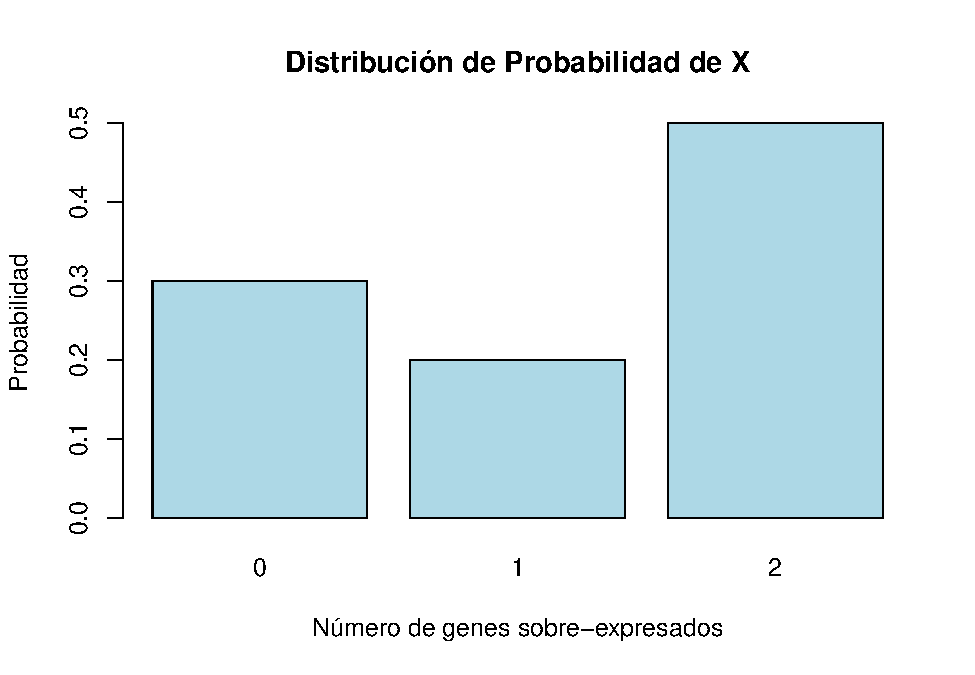
\includegraphics{EjerciciosInferenciaEstadistica_files/figure-latex/unnamed-chunk-7-1.pdf}

\subsubsection{Esperanza y varianza}\label{esperanza-y-varianza}

La \textbf{esperanza} (o valor esperado) de una variable aleatoria discreta \(X\) se calcula como:

\[
E(X) = \sum_{x} x \cdot P(X = x)
\]

Sustituyendo los valores:

\[
E(X) = 0 \cdot 0.30 + 1 \cdot 0.20 + 2 \cdot 0.50 = 0 + 0.20 + 1.00 = 1.20
\]

La \textbf{varianza} de \(X\) se calcula como:

\[
\text{Var}(X) = E(X^2) - [E(X)]^2
\]

Primero calculamos \(E(X^2)\):

\[
E(X^2) = \sum_{x} x^2 \cdot P(X = x)
\]

\[
E(X^2) = 0^2 \cdot 0.30 + 1^2 \cdot 0.20 + 2^2 \cdot 0.50 = 0 + 0.20 + 2.00 = 2.20
\]

Entonces, la varianza es:

\[
\text{Var}(X) = 2.20 - (1.20)^2 = 2.20 - 1.44 = 0.76
\]

Verificamos los cálculos con R:

\begin{Shaded}
\begin{Highlighting}[]
\CommentTok{\# Calcular esperanza y varianza}
\NormalTok{esperanza }\OtherTok{\textless{}{-}} \FunctionTok{sum}\NormalTok{(X\_values }\SpecialCharTok{*}\NormalTok{ probabilities)}
\NormalTok{esperanza\_cuadrado }\OtherTok{\textless{}{-}} \FunctionTok{sum}\NormalTok{(X\_values}\SpecialCharTok{\^{}}\DecValTok{2} \SpecialCharTok{*}\NormalTok{ probabilities)}

\NormalTok{varianza }\OtherTok{\textless{}{-}}\NormalTok{ esperanza\_cuadrado }\SpecialCharTok{{-}}\NormalTok{ esperanza}\SpecialCharTok{\^{}}\DecValTok{2}

\NormalTok{esperanza}
\end{Highlighting}
\end{Shaded}

\begin{verbatim}
## [1] 1.2
\end{verbatim}

\begin{Shaded}
\begin{Highlighting}[]
\NormalTok{varianza}
\end{Highlighting}
\end{Shaded}

\begin{verbatim}
## [1] 0.76
\end{verbatim}

\subsection{Ejercicio 2.2}\label{ejercicio-2.2}

Para describir el número de mutaciones presentes en un volumen estándar de un tumor unos investigadores han propuesto el modelo siguiente

\[
p(x)=\frac{K}{2+x}, x=0,1,2,3,4,5
\]

\begin{enumerate}
\def\labelenumi{\arabic{enumi}.}
\tightlist
\item
  Determinar qué valor debe de tener \(K\) para que \(p(x)\) sea una función de masa de probabilidad
\item
  Calcular su esperanza y su varianza
\item
  Calcular las probabilidades de los sucesos:

  \begin{itemize}
  \tightlist
  \item
    1 Un tumor presenta exactamente tres mutaciones
  \item
    2 Un tumor presenta al menos una mutación
  \item
    3 Un tumor presenta como máximo dos mutaciones.
  \end{itemize}
\end{enumerate}

\textbf{SOLUCIÓN}

Se considera el modelo para la distribución de probabilidades de mutaciones en un tumor dado por:

\[
p(x)=\frac{K}{2+x}, x=0,1,2,3,4,5
\]

\subsubsection{\texorpdfstring{Valor de \(K\)}{Valor de K}}\label{valor-de-k}

Para que \(p(x)\) sea una función de masa de probabilidad, la suma de todas las probabilidades debe ser igual a 1. Es decir:

\[
\sum_{x=0}^{5} p(x) = 1
\]

Sustituyendo la fórmula de \(p(x)\):

\[
\sum_{x=0}^{5} \frac{K}{2+x} = 1
\]

Simplificamos la suma:

\[
K \sum_{x=0}^{5} \frac{1}{2+x} = 1
\]

La suma es:

\[
\sum_{x=0}^{5} \frac{1}{2+x} = \frac{1}{2} + \frac{1}{3} + \frac{1}{4} + \frac{1}{5} + \frac{1}{6} + \frac{1}{7}
\]

Podemos calcular esta suma numéricamente en R:

\begin{Shaded}
\begin{Highlighting}[]
\CommentTok{\# Valores de la suma}
\NormalTok{suma }\OtherTok{\textless{}{-}} \FunctionTok{sum}\NormalTok{(}\DecValTok{1} \SpecialCharTok{/}\NormalTok{ (}\DecValTok{2} \SpecialCharTok{+} \DecValTok{0}\SpecialCharTok{:}\DecValTok{5}\NormalTok{))}

\CommentTok{\# Calcular el valor de K}
\NormalTok{K }\OtherTok{\textless{}{-}} \DecValTok{1} \SpecialCharTok{/}\NormalTok{ suma}
\NormalTok{K}
\end{Highlighting}
\end{Shaded}

\begin{verbatim}
## [1] 0.6278027
\end{verbatim}

\subsubsection{Esperanza y la varianza}\label{esperanza-y-la-varianza}

La \textbf{esperanza} de \(X\) se calcula como:

\[
E(X) = \sum_{x=0}^{5} x \cdot p(x) = \sum_{x=0}^{5} x \cdot \frac{K}{2+x}
\]

La \textbf{varianza} se calcula usando:

\[
\text{Var}(X) = E(X^2) - [E(X)]^2
\]

Para esto, primero calculamos \(E(X^2)\):

\[
E(X^2) = \sum_{x=0}^{5} x^2 \cdot p(x) = \sum_{x=0}^{5} x^2 \cdot \frac{K}{2+x}
\]

Podemos calcular la esperanza y la varianza en R de la siguiente forma:

\begin{Shaded}
\begin{Highlighting}[]
\CommentTok{\# Calcular la esperanza}
\NormalTok{esperanza }\OtherTok{\textless{}{-}} \FunctionTok{sum}\NormalTok{((}\DecValTok{0}\SpecialCharTok{:}\DecValTok{5}\NormalTok{) }\SpecialCharTok{*}\NormalTok{ K }\SpecialCharTok{/}\NormalTok{ (}\DecValTok{2} \SpecialCharTok{+} \DecValTok{0}\SpecialCharTok{:}\DecValTok{5}\NormalTok{))}

\CommentTok{\# Calcular la esperanza al cuadrado}
\NormalTok{esperanza\_cuadrado }\OtherTok{\textless{}{-}} \FunctionTok{sum}\NormalTok{((}\DecValTok{0}\SpecialCharTok{:}\DecValTok{5}\NormalTok{)}\SpecialCharTok{\^{}}\DecValTok{2} \SpecialCharTok{*}\NormalTok{ K }\SpecialCharTok{/}\NormalTok{ (}\DecValTok{2} \SpecialCharTok{+} \DecValTok{0}\SpecialCharTok{:}\DecValTok{5}\NormalTok{))}

\CommentTok{\# Calcular la varianza}
\NormalTok{varianza }\OtherTok{\textless{}{-}}\NormalTok{ esperanza\_cuadrado }\SpecialCharTok{{-}}\NormalTok{ esperanza}\SpecialCharTok{\^{}}\DecValTok{2}

\NormalTok{esperanza}
\end{Highlighting}
\end{Shaded}

\begin{verbatim}
## [1] 1.766816
\end{verbatim}

\begin{Shaded}
\begin{Highlighting}[]
\NormalTok{varianza}
\end{Highlighting}
\end{Shaded}

\begin{verbatim}
## [1] 2.761769
\end{verbatim}

\subsubsection{Probabilidades}\label{probabilidades}

\textbf{Probabilidad de que un tumor presente exactamente tres mutaciones}

La probabilidad de que \(X = 3\) es:

\[
P(X = 3) = p(3) = \frac{K}{2+3}
\]

Podemos calcularlo en R:

\begin{Shaded}
\begin{Highlighting}[]
\CommentTok{\# Probabilidad de X = 3}
\NormalTok{P\_X\_3 }\OtherTok{\textless{}{-}}\NormalTok{ K }\SpecialCharTok{/}\NormalTok{ (}\DecValTok{2} \SpecialCharTok{+} \DecValTok{3}\NormalTok{)}
\NormalTok{P\_X\_3}
\end{Highlighting}
\end{Shaded}

\begin{verbatim}
## [1] 0.1255605
\end{verbatim}

\textbf{Probabilidad de que un tumor presente al menos una mutación}

La probabilidad de que \(X \geq 1\) es:

\[
P(X \geq 1) = 1 - P(X = 0)
\]

Podemos calcularlo en R:

\begin{Shaded}
\begin{Highlighting}[]
\CommentTok{\# Probabilidad de X \textgreater{}= 1}
\NormalTok{P\_X\_1 }\OtherTok{\textless{}{-}} \DecValTok{1} \SpecialCharTok{{-}}\NormalTok{ K }\SpecialCharTok{/}\NormalTok{ (}\DecValTok{2} \SpecialCharTok{+} \DecValTok{0}\NormalTok{)}
\NormalTok{P\_X\_1}
\end{Highlighting}
\end{Shaded}

\begin{verbatim}
## [1] 0.6860987
\end{verbatim}

\textbf{Probabilidad de que un tumor presente como máximo dos mutaciones}

La probabilidad de que \(X \leq 2\) es:

\[
P(X \leq 2) = P(X = 0) + P(X = 1) + P(X = 2)
\]

Podemos calcularlo en R:

\begin{Shaded}
\begin{Highlighting}[]
\CommentTok{\# Probabilidad de X \textless{}= 2}
\NormalTok{P\_X\_2 }\OtherTok{\textless{}{-}} \FunctionTok{sum}\NormalTok{(K }\SpecialCharTok{/}\NormalTok{ (}\DecValTok{2} \SpecialCharTok{+} \DecValTok{0}\SpecialCharTok{:}\DecValTok{2}\NormalTok{))}
\NormalTok{P\_X\_2}
\end{Highlighting}
\end{Shaded}

\begin{verbatim}
## [1] 0.6801196
\end{verbatim}

\subsection{Ejercicio 2.3}\label{ejercicio-2.3}

Un modelo simplificado del tiempo de supervivencia, en años, tras un diagnóstico de una variante de leucemia es el siguiente:

\[
f_{x}(x)=-0.5 \cdot x+1, \quad \text { donde } \quad 0 \leq x \leq 2
\]

\begin{enumerate}
\def\labelenumi{\arabic{enumi}.}
\item
  Comprobar que \(f_{X}\) es una densidad. Representarla gráficamente.
\item
  Calcular \(\mathrm{F}_{\mathrm{X}} \mathrm{y}\) representarla gráficamente.
\item
  Calcular \(P(X \geq 1), P(X>1), P(X=1), f_{x}(1)\).
\item
  Calcular la probabilidad de que un individuo diagnosticado con leucemia sobreviva :
\end{enumerate}

\begin{enumerate}
\def\labelenumi{(\roman{enumi})}
\tightlist
\item
  menos de seis meses, (ii) entre seis meses y un año, (iii) más de dos años.
\end{enumerate}

\begin{enumerate}
\def\labelenumi{\arabic{enumi}.}
\setcounter{enumi}{4}
\item
  Calcular \(E(X)\) i \(\operatorname{Var}(X)\).
\item
  En vista que el modelo anterior no ha resultado satisfactorio una bioestadística ha propuesto un modelo alternativo consistente en modelizar la variable como:
\end{enumerate}

\[
g_{X}(x)=\exp (-k x), \text { dondex } \geq 0
\]

Calcular la constante \(k\) para que \(\mathrm{g}_{\mathrm{x}}\) sea una función de densidad de probabilidad. Repetir los cálculos de los apartados b), c), d) y e) con el nuevo modelo. Discutir adecuación de ambos modelos a una situación real.

\textbf{SOLUCIÓN}

\subsubsection{\texorpdfstring{\(f_X(x)\) es una densidad}{f\_X(x) es una densidad}}\label{f_xx-es-una-densidad}

Para comprobar que \(f_X(x)\) es una función de densidad, necesitamos verificar que cumple las dos condiciones básicas:

\begin{enumerate}
\def\labelenumi{\arabic{enumi}.}
\tightlist
\item
  \(f_X(x) \geq 0\) para todo \(x\) en su dominio.
\item
  La integral de \(f_X(x)\) sobre todo su dominio debe ser 1, es decir:
\end{enumerate}

\[
\int_0^2 f_X(x) \, dx = 1
\]

La función de densidad dada es \(f_X(x) = -0.5 \cdot x + 1\) con \(0 \leq x \leq 2\).

Primero, comprobamos que \(f_X(x) \geq 0\) para \(x \in [0, 2]\). Evaluamos los valores extremos:

\begin{itemize}
\tightlist
\item
  \(f_X(0) = -0.5 \cdot 0 + 1 = 1\)
\item
  \(f_X(2) = -0.5 \cdot 2 + 1 = 0\)
\end{itemize}

La función es no negativa en el intervalo dado.

Ahora, calculamos la integral:

\[
\int_0^2 (-0.5 \cdot x + 1) \, dx = \left[ -0.25 \cdot x^2 + x \right]_0^2 = (-0.25 \cdot 4 + 2) - (0) = 1
\]

Por lo tanto, \(f_X(x)\) cumple con ambas condiciones y es una función de densidad.

\subsubsection{\texorpdfstring{Gráfica de \(f_X(x)\)}{Gráfica de f\_X(x)}}\label{gruxe1fica-de-f_xx}

\begin{Shaded}
\begin{Highlighting}[]
\CommentTok{\# R code to plot the density function}
\NormalTok{f\_x }\OtherTok{\textless{}{-}} \ControlFlowTok{function}\NormalTok{(x) }\SpecialCharTok{{-}}\FloatTok{0.5} \SpecialCharTok{*}\NormalTok{ x }\SpecialCharTok{+} \DecValTok{1}
\FunctionTok{curve}\NormalTok{(f\_x, }\AttributeTok{from =} \DecValTok{0}\NormalTok{, }\AttributeTok{to =} \DecValTok{2}\NormalTok{, }\AttributeTok{col =} \StringTok{"blue"}\NormalTok{, }\AttributeTok{lwd =} \DecValTok{2}\NormalTok{, }\AttributeTok{ylab =} \StringTok{"f\_X(x)"}\NormalTok{, }\AttributeTok{xlab =} \StringTok{"x"}\NormalTok{,}
      \AttributeTok{main =} \StringTok{"Densidad f\_X(x)"}\NormalTok{)}
\end{Highlighting}
\end{Shaded}

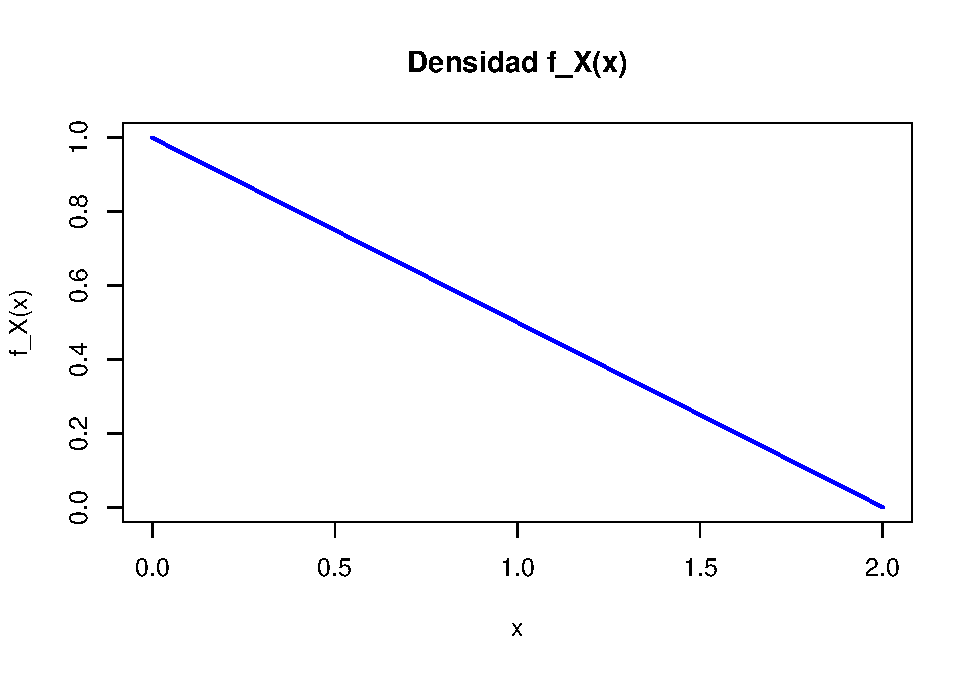
\includegraphics{EjerciciosInferenciaEstadistica_files/figure-latex/unnamed-chunk-14-1.pdf}

\subsubsection{Función de distribución}\label{funciuxf3n-de-distribuciuxf3n}

\textbf{Calcular \(F_X(x)\) y representarla gráficamente}

La función de distribución acumulada (CDF) \(F_X(x)\) se obtiene integrando la función de densidad:

\[
F_X(x) = \int_0^x (-0.5 \cdot t + 1) \, dt
\]

Para \(x \in [0, 2]\), tenemos:

\[
F_X(x) = \left[-0.25 \cdot t^2 + t\right]_0^x = -0.25 \cdot x^2 + x
\]

Para \(x < 0\), \(F_X(x) = 0\), y para \(x > 2\), \(F_X(x) = 1\).

\textbf{Gráfica de \(F_X(x)\)ç}

\begin{Shaded}
\begin{Highlighting}[]
\CommentTok{\# R code to plot the CDF function}
\NormalTok{F\_x }\OtherTok{\textless{}{-}} \ControlFlowTok{function}\NormalTok{(x) }\FunctionTok{ifelse}\NormalTok{(x }\SpecialCharTok{\textless{}} \DecValTok{0}\NormalTok{, }\DecValTok{0}\NormalTok{, }\FunctionTok{ifelse}\NormalTok{(x }\SpecialCharTok{\textgreater{}} \DecValTok{2}\NormalTok{, }\DecValTok{1}\NormalTok{, }\SpecialCharTok{{-}}\FloatTok{0.25} \SpecialCharTok{*}\NormalTok{ x}\SpecialCharTok{\^{}}\DecValTok{2} \SpecialCharTok{+}\NormalTok{ x))}
\FunctionTok{curve}\NormalTok{(F\_x, }\AttributeTok{from =} \SpecialCharTok{{-}}\DecValTok{1}\NormalTok{, }\AttributeTok{to =} \DecValTok{3}\NormalTok{, }\AttributeTok{col =} \StringTok{"red"}\NormalTok{, }\AttributeTok{lwd =} \DecValTok{2}\NormalTok{, }\AttributeTok{ylab =} \StringTok{"F\_X(x)"}\NormalTok{, }\AttributeTok{xlab =} \StringTok{"x"}\NormalTok{,}
      \AttributeTok{main =} \StringTok{"Distribución acumulada F\_X(x)"}\NormalTok{)}
\end{Highlighting}
\end{Shaded}

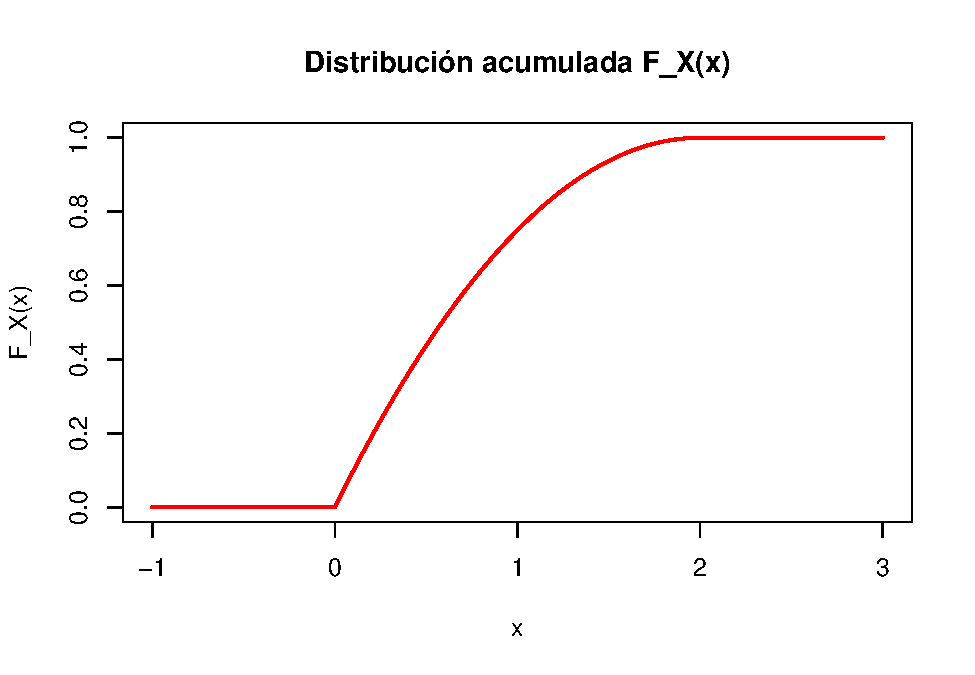
\includegraphics{EjerciciosInferenciaEstadistica_files/figure-latex/unnamed-chunk-15-1.pdf}

\subsubsection{\texorpdfstring{Probabilidades y \(f_X(1)\)}{Probabilidades y f\_X(1)}}\label{probabilidades-y-f_x1}

\begin{enumerate}
\def\labelenumi{\arabic{enumi}.}
\tightlist
\item
  \(P(X \geq 1) = 1 - F_X(1)\):
\end{enumerate}

\[
F_X(1) = -0.25 \cdot 1^2 + 1 = 0.75
\]
Por lo tanto, \(P(X \geq 1) = 1 - 0.75 = 0.25\).

\begin{enumerate}
\def\labelenumi{\arabic{enumi}.}
\setcounter{enumi}{1}
\item
  \(P(X > 1)\): Como \(X\) es una variable continua, \(P(X > 1) = P(X \geq 1) = 0.25\).
\item
  \(P(X = 1)\): Para una variable continua, la probabilidad puntual es 0, es decir, \(P(X = 1) = 0\).
\item
  \(f_X(1)\):
\end{enumerate}

\[
f_X(1) = -0.5 \cdot 1 + 1 = 0.5
\]

\subsubsection{Probabilidad de supervivencia}\label{probabilidad-de-supervivencia}

\begin{enumerate}
\def\labelenumi{\arabic{enumi}.}
\tightlist
\item
  Menos de seis meses (\(x = 0.5\)):
\end{enumerate}

\[
P(X < 0.5) = F_X(0.5) = -0.25 \cdot 0.5^2 + 0.5 = 0.4375
\]

\begin{enumerate}
\def\labelenumi{\arabic{enumi}.}
\setcounter{enumi}{1}
\tightlist
\item
  Entre seis meses y un año (\(x \in [0.5, 1]\)):
\end{enumerate}

\[
P(0.5 \leq X \leq 1) = F_X(1) - F_X(0.5) = 0.75 - 0.375 = 0.375
\]

\begin{enumerate}
\def\labelenumi{\arabic{enumi}.}
\setcounter{enumi}{2}
\tightlist
\item
  Más de dos años (\(x > 2\)): Como el dominio de \(X\) es \([0, 2]\), \(P(X > 2) = 0\).
\end{enumerate}

\subsubsection{\texorpdfstring{\(E(X)\) y \(\operatorname{Var}(X)\)}{E(X) y \textbackslash operatorname\{Var\}(X)}}\label{ex-y-operatornamevarx}

\begin{enumerate}
\def\labelenumi{\arabic{enumi}.}
\tightlist
\item
  La esperanza de \(X\) es:
\end{enumerate}

\[
E(X) = \int_0^2 x \cdot f_X(x) \, dx = \int_0^2 x \cdot (-0.5 \cdot x + 1) \, dx
\]

Desarrollamos:

\[
E(X) = \int_0^2 (-0.5 \cdot x^2 + x) \, dx = \left[-\frac{0.5}{3} \cdot x^3 + 0.5 \cdot x^2\right]_0^2
\]

Calculamos:

\[
E(X) = -\frac{0.5}{3} \cdot 8 + 0.5 \cdot 4 = -\frac{4}{3} + 2 = \frac{2}{3}
\]

\begin{enumerate}
\def\labelenumi{\arabic{enumi}.}
\setcounter{enumi}{1}
\tightlist
\item
  La varianza de \(X\) es:
\end{enumerate}

\[
\operatorname{Var}(X) = E(X^2) - E(X)^2
\]

Primero calculamos \(E(X^2)\):

\[
E(X^2) = \int_0^2 x^2 \cdot f_X(x) \, dx = \int_0^2 x^2 \cdot (-0.5 \cdot x + 1) \, dx
\]

Desarrollamos y calculamos:

\[
E(X^2) = \int_0^2 (-0.5 \cdot x^3 + x^2) \, dx = \left[-\frac{0.5}{4} \cdot x^4 + \frac{1}{3} \cdot x^3\right]_0^2
\]

\[
E(X^2) = -\frac{0.5}{4} \cdot 16 + \frac{1}{3} \cdot 8 = -2 + \frac{8}{3} = \frac{2}{3}
\]

Finalmente:

\[
\operatorname{Var}(X) = E(X^2) - E(X)^2 = \frac{2}{3} - \left(\frac{2}{3}\right)^2 = \frac{2}{3} - \frac{4}{9} = \frac{2}{9}
\]

\subsubsection{\texorpdfstring{Modelo alternativo \(g_X(x)\)}{Modelo alternativo g\_X(x)}}\label{modelo-alternativo-g_xx}

Dado el modelo alternativo \(g_X(x) = \exp(-k \cdot x)\) para \(x \geq 0\), la constante \(k\) se determina imponiendo que la integral de la función de densidad debe ser 1:

\[
\int_0^\infty \exp(-k \cdot x) \, dx = 1
\]

Resolviendo:

\[
\frac{1}{k} = 1 \implies k = 1
\]

Por lo tanto, el nuevo modelo de densidad es \(g_X(x) = \exp(-x)\).

\subsection{Ejercicio 2.4}\label{ejercicio-2.4}

Para estudiar la regulación hormonal de una línea metabólica se inyectan ratas albinas con un fármaco que inhibe la síntesis de proteínas del organismo. En general, 4 de cada 20 ratas mueren a causa del fármaco antes de que el experimento haya concluido. Si se trata a 10 animales con el fármaco, ¿cuál es la probabilidad de que al menos 8 lleguen vivas al final del experimento?

\textbf{SOLUCION}

En este problema en el que tenemos grupos de 10 animales independientes, cada uno de los cuales puede sobrevivir o no resulta apropiada \textbf{la distribución binomial}.

\begin{itemize}
\item
  La probabilidad de que una rata sobreviva al fármaco es \(p = \frac{16}{20} = 0.8\), dado que 4 de cada 20 ratas mueren.
\item
  El experimento se realiza con 10 ratas, por lo que tenemos \(n = 10\).
\item
  Queremos calcular la probabilidad de que al menos 8 ratas sobrevivan. Matemáticamente, esto corresponde a:
\end{itemize}

\[
P(X \geq 8)
\]

donde \(X\) es el número de ratas que sobreviven y sigue una \textbf{distribución binomial}:

\[
X \sim \text{Binomial}(n=10, p=0.8)
\]

\subsubsection{Cálculo de la probabilidad}\label{cuxe1lculo-de-la-probabilidad}

La probabilidad de que exactamente \(k\) ratas sobrevivan está dada por la fórmula de la binomial:

\[
P(X = k) = \binom{n}{k} p^k (1 - p)^{n-k}
\]

Para responder la pregunta debemos calcular:

\[
P(X \geq 8) = P(X = 8) + P(X = 9) + P(X = 10)
\]
Esto puede calcularse:

\begin{itemize}
\tightlist
\item
  directamente usando la función de probabilidad acumulada implementada en R
\item
  indirectamente calculando las probabilidades individuales y sumándolas.
\end{itemize}

En todo caso debemos recordar que al tratarse de una variable discreta si queremos usar \(F_X(x)\) para calcular \(P(X\geq k)\) deberemos tener en cuenta que:
\[
P(X\geq k) = 1-P(X\leq k-1)
\]
En primer lugar calculamos esta suma utilizando la función de masa de probabilidad:

\begin{Shaded}
\begin{Highlighting}[]
\CommentTok{\# Parámetros del problema}
\NormalTok{n }\OtherTok{\textless{}{-}} \DecValTok{10}
\NormalTok{p }\OtherTok{\textless{}{-}} \FloatTok{0.8}

\CommentTok{\# Probabilidades P(X = 8), P(X = 9) y P(X = 10)}
\NormalTok{prob\_8 }\OtherTok{\textless{}{-}} \FunctionTok{dbinom}\NormalTok{(}\DecValTok{8}\NormalTok{, }\AttributeTok{size =}\NormalTok{ n, }\AttributeTok{prob =}\NormalTok{ p)}
\NormalTok{prob\_9 }\OtherTok{\textless{}{-}} \FunctionTok{dbinom}\NormalTok{(}\DecValTok{9}\NormalTok{, }\AttributeTok{size =}\NormalTok{ n, }\AttributeTok{prob =}\NormalTok{ p)}
\NormalTok{prob\_10 }\OtherTok{\textless{}{-}} \FunctionTok{dbinom}\NormalTok{(}\DecValTok{10}\NormalTok{, }\AttributeTok{size =}\NormalTok{ n, }\AttributeTok{prob =}\NormalTok{ p)}

\CommentTok{\# Probabilidad total P(X \textgreater{}= 8)}
\NormalTok{prob\_total }\OtherTok{\textless{}{-}}\NormalTok{ prob\_8 }\SpecialCharTok{+}\NormalTok{ prob\_9 }\SpecialCharTok{+}\NormalTok{ prob\_10}
\NormalTok{prob\_total}
\end{Highlighting}
\end{Shaded}

\begin{verbatim}
## [1] 0.6777995
\end{verbatim}

Si usamos la funcion de distribución, \texttt{pbinom}

\begin{Shaded}
\begin{Highlighting}[]
\DecValTok{1}\SpecialCharTok{{-}}\FunctionTok{pbinom}\NormalTok{ (}\DecValTok{7}\NormalTok{, }\AttributeTok{size =}\NormalTok{ n, }\AttributeTok{prob =}\NormalTok{ p)}
\end{Highlighting}
\end{Shaded}

\begin{verbatim}
## [1] 0.6777995
\end{verbatim}

Naturalmente ambos resultados coinciden. Obsérvese que al ser \(p=0.8\) valores altos resultan bastante probables, con lo que la

\subsection{Ejercicio 2.5}\label{ejercicio-2.5}

En una cierta población se ha observado un número medio anual de 12 muertes por cáncer de pulmón. Si el número de muertes causadas por la enfermedad sigue una distribución de Poisson, ¿cuál es la probabilidad de que durante el año en curso:
1. haya exactamente 10 muertes por cáncer de pulmón?
2. 15 o más personas mueran a causa de la enfermedad?
3. 10 o menos personas mueran a causa de la enfermedad?

El número de muertes por cáncer de pulmón sigue una distribución de Poisson, que se usa para modelar la ocurrencia de eventos discretos dentro de un intervalo de tiempo, donde el valor esperado es proporcional al tamaño del intervalo. En este caso, el valor esperado es el número medio de muertes por año, que es 12. La función de masa de probabilidad (PMF) de una variable aleatoria \(X\) con distribución de Poisson y parámetro \(\lambda\) es:

\[ P(X = k) = \frac{\lambda^k e^{-\lambda}}{k!} \]

donde \(k\) es el número de eventos, \(\lambda\) es el valor esperado (12 en nuestro caso) y \(k!\) es el factorial de \(k\). Usaremos este modelo para resolver los apartados.

\subsubsection{Probabilidad de que haya exactamente 10 muertes}\label{probabilidad-de-que-haya-exactamente-10-muertes}

La probabilidad de observar exactamente \(k = 10\) muertes se puede calcular usando la PMF de la distribución de Poisson con \(\lambda = 12\):

\[ P(X = 10) = \frac{12^{10} e^{-12}}{10!} \]

Podemos calcular este valor con R.

\begin{Shaded}
\begin{Highlighting}[]
\NormalTok{lambda }\OtherTok{\textless{}{-}} \DecValTok{12}
\NormalTok{k }\OtherTok{\textless{}{-}} \DecValTok{10}
\NormalTok{prob\_10\_muertes }\OtherTok{\textless{}{-}} \FunctionTok{dpois}\NormalTok{(k, lambda)}
\NormalTok{prob\_10\_muertes}
\end{Highlighting}
\end{Shaded}

\begin{verbatim}
## [1] 0.1048373
\end{verbatim}

\subsubsection{Probabilidad de que 15 o más personas mueran}\label{probabilidad-de-que-15-o-muxe1s-personas-mueran}

Para obtener la probabilidad de que 15 o más personas mueran, necesitamos calcular la probabilidad acumulada de \(X \geq 15\). Esto se puede obtener restando de 1 la probabilidad acumulada de \(X < 15\), es decir:

\[ P(X \geq 15) = 1 - P(X < 15) = 1 - P(X \leq 14) \]

Usamos la función de probabilidad acumulada (CDF) de la Poisson en R.

\begin{Shaded}
\begin{Highlighting}[]
\NormalTok{k\_15 }\OtherTok{\textless{}{-}} \DecValTok{14}
\NormalTok{prob\_15\_o\_mas }\OtherTok{\textless{}{-}} \DecValTok{1} \SpecialCharTok{{-}} \FunctionTok{ppois}\NormalTok{(k\_15, lambda)}
\NormalTok{prob\_15\_o\_mas}
\end{Highlighting}
\end{Shaded}

\begin{verbatim}
## [1] 0.2279755
\end{verbatim}

\subsubsection{Probabilidad de que 10 o menos personas mueran}\label{probabilidad-de-que-10-o-menos-personas-mueran}

La probabilidad de que 10 o menos personas mueran es simplemente la probabilidad acumulada de \(X \leq 10\), que se puede calcular directamente con la CDF de la distribución de Poisson.

\[ P(X \leq 10) \]

Calculamos esto en R:

\begin{Shaded}
\begin{Highlighting}[]
\NormalTok{prob\_10\_o\_menos }\OtherTok{\textless{}{-}} \FunctionTok{ppois}\NormalTok{(k, lambda)}
\NormalTok{prob\_10\_o\_menos}
\end{Highlighting}
\end{Shaded}

\begin{verbatim}
## [1] 0.3472294
\end{verbatim}

\subsubsection{Conclusión}\label{conclusiuxf3n}

\begin{enumerate}
\def\labelenumi{\arabic{enumi}.}
\tightlist
\item
  La probabilidad de que haya exactamente 10 muertes es:
\end{enumerate}

\begin{Shaded}
\begin{Highlighting}[]
\NormalTok{prob\_10\_muertes}
\end{Highlighting}
\end{Shaded}

\begin{verbatim}
## [1] 0.1048373
\end{verbatim}

\begin{enumerate}
\def\labelenumi{\arabic{enumi}.}
\setcounter{enumi}{1}
\tightlist
\item
  La probabilidad de que 15 o más personas mueran es:
\end{enumerate}

\begin{Shaded}
\begin{Highlighting}[]
\NormalTok{prob\_15\_o\_mas}
\end{Highlighting}
\end{Shaded}

\begin{verbatim}
## [1] 0.2279755
\end{verbatim}

\begin{enumerate}
\def\labelenumi{\arabic{enumi}.}
\setcounter{enumi}{2}
\tightlist
\item
  La probabilidad de que 10 o menos personas mueran es:
\end{enumerate}

\begin{Shaded}
\begin{Highlighting}[]
\NormalTok{prob\_10\_o\_menos}
\end{Highlighting}
\end{Shaded}

\begin{verbatim}
## [1] 0.3472294
\end{verbatim}

\subsection{Ejercicio 2.6}\label{ejercicio-2.6}

Los daños a los cromosomas del óvulo o del espermatozoide, pueden causar mutaciones que conducen a abortos, defectos de nacimiento, u otras deficiencias genéticas. Un estudio sobre los efectos teratogénicos de la radiación ha determinado que la probabilidad de que tal mutación se produzca por radiación es del 10\%. El resto son atribuibles a otras causas.
Una vez detectadas 150 mutaciones,

\begin{enumerate}
\def\labelenumi{\arabic{enumi}.}
\tightlist
\item
  ¿cuántas se esperaría que se debiesen a radiaciones?
\item
  ¿Cuál es la probabilidad de que solamente 10 se debiesen a radiaciones?
\end{enumerate}

\textbf{Solución}

Para analizar el número de mutaciones que se deben a radiaciones, podemos considera dos modelos diferentes: uno basado en la distribución binomial y otro en la distribución de Poisson.

\subsubsection{Justificación del uso de distribución binomial}\label{justificaciuxf3n-del-uso-de-distribuciuxf3n-binomial}

La distribución binomial es adecuada cuando tenemos un número fijo de ensayos independientes y cada ensayo tiene dos posibles resultados: éxito (la mutación es debida a radiación) o fracaso (la mutación no es debida a radiación). En cada ensayo, la probabilidad de éxito es constante.

Esto se ajusta perfectamente a las condiciones del problema:
- Hay 150 ensayos independientes (cada mutación observada puede estar o no causada por radiación).
- Cada ensayo tiene dos posibles resultados: mutación por radiación o mutación por otra causa.
- La probabilidad de éxito es constante y pequeña (\(p = 0.1\)).
Por tanto, el número de mutaciones debidas a radiación se puede modelizar bien mediante una distribución binomial \(X \sim \text{Binomial}(n = 150, p = 0.1)\).

\subsubsection{Justificación del uso de distribución de Poisson}\label{justificaciuxf3n-del-uso-de-distribuciuxf3n-de-poisson}

La distribución de Poisson es adecuada para modelar el número de eventos raros que ocurren en un intervalo de tiempo, espacio, o cualquier otra unidad, cuando estos eventos ocurren de forma independiente y su probabilidad de ocurrencia es baja.

En este caso las ``mutaciones debidas a radiación'' pueden considerarse eventos raros dentro de un gran conjunto de mutaciones (150 mutaciones observadas, pero solo un 10\% de ellas son debidas a radiación).

Puede considerarse además, que las mutaciones individuales pueden ocurrir de forma independiente entre sí, ya que la probabilidad de que una mutación se deba a radiación no afecta a la probabilidad de que otra mutación sea causada por radiación.

Estas condiciones son características de los \emph{procesos de Poisson} y por tanto la distribución de Poisson es una elección natural para describir procesos en los que los eventos ocurren de manera aleatoria en un intervalo dado (por ejemplo, en un periodo de tiempo o un espacio), siempre que:

\begin{itemize}
\tightlist
\item
  Los eventos ocurran con una tasa promedio constante (en este caso, la tasa de mutaciones debidas a radiaciones es proporcional a la tasa global de mutaciones, multiplicada por la probabilidad \(p = 0.1\)).
\item
  No haya límite teórico en el número de eventos que puedan ocurrir en un intervalo (aunque observamos un total de 150 mutaciones, teóricamente podríamos seguir detectando más mutaciones).
\end{itemize}

En el modelo de Poisson, el parámetro \(\lambda\) representa la tasa promedio de ocurrencia de los eventos (en este caso, mutaciones debidas a radiación). Si conocemos la tasa promedio de aparición de mutaciones por radiación (\(\lambda = n \cdot p\) en el contexto binomial, pero también se puede calcular directamente si conocemos la tasa de aparición de eventos raros), entonces podemos usar directamente la distribución de Poisson para modelar el número de eventos.

En este caso, \(\lambda = 150 \cdot 0.1 = 15\), que representa el número esperado de mutaciones debidas a radiación en el total observado de mutaciones.

\subsubsection{Aproximación del modelo binomial por el de Poisson}\label{aproximaciuxf3n-del-modelo-binomial-por-el-de-poisson}

La distribución de Poisson puede considerarse una aproximación de la binomial cuando el número de ensayos (\(n\)) es grande y la probabilidad de éxito (\(p\)) es pequeña. En este caso, el número esperado de éxitos, \(n \cdot p\), se mantiene moderado (en este caso, \(n \cdot p = 15\)).

Este resultado que se conoce como \emph{límite de Poisson} establece que si:

\begin{itemize}
\tightlist
\item
  \(n\) es grande (muchos ensayos),
\item
  \(p\) es pequeño (baja probabilidad de éxito),
\item
  el producto \(n \cdot p = \lambda\) es moderado,
\end{itemize}

entonces la binomial \(X \sim \text{Binomial}(n, p)\) se puede aproximar por una distribución de Poisson con parámetro \(\lambda = n \cdot p\).

En este caso:

\begin{itemize}
\tightlist
\item
  \(n = 150\) es suficientemente grande.
\item
  \(p = 0.1\) es pequeño.
\item
  \(n \cdot p = 15\), lo cual es un valor razonable para usar la aproximación de Poisson.
\end{itemize}

Por tanto, el número de mutaciones debidas a radiaciones puede aproximarse por una distribución de Poisson \(X \sim \text{Poisson}(\lambda = 15)\).

\subsubsection{Número esperado de mutaciones}\label{nuxfamero-esperado-de-mutaciones}

En ambos modelos, la esperanza del número de mutaciones debidas a radiaciones es \(E[X] = n \cdot p\). Esto representa el número promedio de mutaciones debidas a radiaciones. Lo calculamos:

\[ E[X] = 150 \cdot 0.1 = 15 \]

Por lo tanto, se espera que alrededor de 15 mutaciones se deban a radiaciones.

\subsubsection{Probabilidad de que exactamente 10 mutaciones se deban a radiaciones}\label{probabilidad-de-que-exactamente-10-mutaciones-se-deban-a-radiaciones}

\paragraph{Usando la distribución Binomial}\label{usando-la-distribuciuxf3n-binomial}

La probabilidad de que exactamente 10 mutaciones se deban a radiaciones se puede calcular usando la PMF de la binomial:

\[ P(X = 10) = \binom{150}{10} (0.1)^{10} (0.9)^{140} \]

Usando R tenemos:

\begin{Shaded}
\begin{Highlighting}[]
\NormalTok{n }\OtherTok{\textless{}{-}} \DecValTok{150}
\NormalTok{p }\OtherTok{\textless{}{-}} \FloatTok{0.1}
\NormalTok{k }\OtherTok{\textless{}{-}} \DecValTok{10}
\NormalTok{prob\_binom\_10 }\OtherTok{\textless{}{-}} \FunctionTok{dbinom}\NormalTok{(k, n, p)}
\NormalTok{prob\_binom\_10}
\end{Highlighting}
\end{Shaded}

\begin{verbatim}
## [1] 0.04591681
\end{verbatim}

\paragraph{Usando la aproximación de Poisson}\label{usando-la-aproximaciuxf3n-de-poisson}

La distribución de Poisson con \(\lambda = n \cdot p = 15\) también se puede usar para aproximar esta probabilidad. La probabilidad de obtener exactamente 10 mutaciones se calcula como:

\[ P(X = 10) = \frac{15^{10} e^{-15}}{10!} \]

Con R:

\begin{Shaded}
\begin{Highlighting}[]
\NormalTok{lambda }\OtherTok{\textless{}{-}} \DecValTok{15}
\NormalTok{prob\_pois\_10 }\OtherTok{\textless{}{-}} \FunctionTok{dpois}\NormalTok{(k, lambda)}
\NormalTok{prob\_pois\_10}
\end{Highlighting}
\end{Shaded}

\begin{verbatim}
## [1] 0.04861075
\end{verbatim}

\subsubsection{Conclusión}\label{conclusiuxf3n-1}

\begin{itemize}
\item
  Se espera que 15 de las 150 mutaciones se deban a radiaciones.
\item
  La probabilidad de que exactamente 10 mutaciones se deban a radiaciones es:

  \begin{itemize}
  \tightlist
  \item
    Usando la distribución binomial:
  \end{itemize}

\begin{Shaded}
\begin{Highlighting}[]
\NormalTok{prob\_binom\_10}
\end{Highlighting}
\end{Shaded}

\begin{verbatim}
## [1] 0.04591681
\end{verbatim}

  \begin{itemize}
  \tightlist
  \item
    Usando la aproximación de Poisson:
  \end{itemize}

\begin{Shaded}
\begin{Highlighting}[]
\NormalTok{prob\_pois\_10}
\end{Highlighting}
\end{Shaded}

\begin{verbatim}
## [1] 0.04861075
\end{verbatim}
\end{itemize}

Ambos métodos dan resultados similares, pero el modelo de Poisson es útil para simplificar los cálculos cuando el número total de mutaciones es grande y la probabilidad de cada evento es pequeña.

\subsection{Ejercicio 2.7}\label{ejercicio-2.7}

Entre los diabéticos, el nivel de glucosa en sangre \(X\), en ayunas, puede suponerse de distribución aproximadamente normal, con media \(106 \mathrm{mg} / 100 \mathrm{ml}\) y desviación típica \(8 \mathrm{mg} / 100 \mathrm{ml}\), es decir : \(X \sim N\left(\mu=106, \sigma^{2}=64\right)\).

Hallar;
1. El porcentaje de diabéticos con niveles de glucosa inferiores a 120 ( \(P[X \leq 120]\)
2. ¿Qué porcentaje de diabéticos tienen niveles comprendidos entre 90 y 120?
3. Hallar el nivel de glucosa ``p25'', caracterizado por la propiedad de que el \(25 \%\) de todos los diabéticos tiene un nivel de glucosa en ayunas inferior o igual a \(x\).

\textbf{SOLUCIÓN}

Según el enunciado el nivel de glucosa \(X\) se distribuye según una distribución normal con media \(\mu = 106\) y varianza \(\sigma^2 = 64\), es decir, \(X \sim N(106, 64)\), o equivalentemente \(X \sim N(106, 8^2)\).

\subsubsection{\texorpdfstring{Porcentaje de diabéticos con niveles de glucosa inferiores a 120 (\(P[X \leq 120]\))}{Porcentaje de diabéticos con niveles de glucosa inferiores a 120 (P{[}X \textbackslash leq 120{]})}}\label{porcentaje-de-diabuxe9ticos-con-niveles-de-glucosa-inferiores-a-120-px-leq-120}

Para calcular esta probabilidad, necesitamos estandarizar la variable \(X\) a una normal estándar \(Z \sim N(0, 1)\). La fórmula de estandarización es:

\[ Z = \frac{X - \mu}{\sigma} \]

Sustituyendo los valores de \(\mu = 106\) y \(\sigma = 8\):

\[ Z = \frac{120 - 106}{8} = 1.75 \]

Ahora calculamos \(P(Z \leq 1.75)\), es decir, la probabilidad de que la variable estándar normal sea menor o igual que 1.75. Esta probabilidad la obtenemos a partir de la tabla de la normal estándar o usando R.

\begin{Shaded}
\begin{Highlighting}[]
\CommentTok{\# Calculamos la probabilidad con la función pnorm}
\NormalTok{p1 }\OtherTok{\textless{}{-}} \FunctionTok{pnorm}\NormalTok{(}\FloatTok{1.75}\NormalTok{)}
\NormalTok{p1}
\end{Highlighting}
\end{Shaded}

\begin{verbatim}
## [1] 0.9599408
\end{verbatim}

\subsubsection{Porcentaje de diabéticos con niveles de glucosa comprendidos entre 90 y 120}\label{porcentaje-de-diabuxe9ticos-con-niveles-de-glucosa-comprendidos-entre-90-y-120}

En este caso queremos calcular \(P(90 \leq X \leq 120)\). Para hacerlo, calculamos las probabilidades individuales de \(P(X \leq 120)\) y \(P(X \leq 90)\), y restamos la segunda de la primera:

\[ P(90 \leq X \leq 120) = P(X \leq 120) - P(X \leq 90) \]

Primero estandarizamos ambas variables:

\[ Z_{120} = \frac{120 - 106}{8} = 1.75 \]
\[ Z_{90} = \frac{90 - 106}{8} = -2.00 \]

Ahora calculamos \(P(Z \leq 1.75)\) y \(P(Z \leq -2.00)\) usando R.

\begin{Shaded}
\begin{Highlighting}[]
\CommentTok{\# Calculamos ambas probabilidades}
\NormalTok{p2\_120 }\OtherTok{\textless{}{-}} \FunctionTok{pnorm}\NormalTok{(}\FloatTok{1.75}\NormalTok{)}
\NormalTok{p2\_90 }\OtherTok{\textless{}{-}} \FunctionTok{pnorm}\NormalTok{(}\SpecialCharTok{{-}}\FloatTok{2.00}\NormalTok{)}
\NormalTok{p2 }\OtherTok{\textless{}{-}}\NormalTok{ p2\_120 }\SpecialCharTok{{-}}\NormalTok{ p2\_90}
\NormalTok{p2}
\end{Highlighting}
\end{Shaded}

\begin{verbatim}
## [1] 0.9371907
\end{verbatim}

\subsubsection{Hallar el nivel de glucosa ``p25''}\label{hallar-el-nivel-de-glucosa-p25}

Para encontrar el percentil 25 de la distribución, necesitamos resolver la ecuación:

\[ P(X \leq p_{25}) = 0.25 \]

Sabemos que \(X \sim N(106, 64)\), así que estandarizamos el valor \(p_{25}\):

\[ Z_{p25} = \frac{p_{25} - 106}{8} \]

Luego, encontramos el valor de \(Z_{p25}\) que corresponde al percentil 25 de la distribución normal estándar, es decir, \(P(Z \leq Z_{p25}) = 0.25\). Esto lo obtenemos con la función inversa de la distribución normal estándar.

\begin{Shaded}
\begin{Highlighting}[]
\CommentTok{\# Calculamos el valor z correspondiente al percentil 25}
\NormalTok{z\_p25 }\OtherTok{\textless{}{-}} \FunctionTok{qnorm}\NormalTok{(}\FloatTok{0.25}\NormalTok{)}
\CommentTok{\# Calculamos el p25 en la escala original}
\NormalTok{p25 }\OtherTok{\textless{}{-}} \DecValTok{106} \SpecialCharTok{+}\NormalTok{ z\_p25 }\SpecialCharTok{*} \DecValTok{8}
\NormalTok{p25}
\end{Highlighting}
\end{Shaded}

\begin{verbatim}
## [1] 100.6041
\end{verbatim}

\subsubsection{Resumen de resultados:}\label{resumen-de-resultados}

\begin{enumerate}
\def\labelenumi{\arabic{enumi}.}
\tightlist
\item
  La probabilidad de que el nivel de glucosa sea menor o igual a 120 es aproximadamente:
\end{enumerate}

\[ P[X \leq 120] = 0.9599 \]

\begin{enumerate}
\def\labelenumi{\arabic{enumi}.}
\setcounter{enumi}{1}
\tightlist
\item
  El porcentaje de diabéticos con niveles de glucosa comprendidos entre 90 y 120 es aproximadamente:
\end{enumerate}

\[ P[90 \leq X \leq 120] = 0.9104 \]

\begin{enumerate}
\def\labelenumi{\arabic{enumi}.}
\setcounter{enumi}{2}
\tightlist
\item
  El nivel de glucosa correspondiente al percentil 25, es decir, el valor \(p_{25}\), es aproximadamente:
\end{enumerate}

\[ p_{25} \approx 100.61 \, \mathrm{mg/100ml} \]

\subsection{Ejercicio 28}\label{ejercicio-28}

Se supone que la glucemia basal en individuos sanos, \(X_{s}\) sigue una distribución \(X \sim N(\mu=80, \sigma=10)\), mientras que en los diabéticos \(X_{d}\), sigue una distribución \(X \sim N(\mu=160, \sigma=31.4)\). Si se conviene en clasificar como sanos al \(2 \%\) de los diabéticos:
a) ¿Por debajo de qué valor se considera sano a un individuo? ¿Cuántos sanos serán clasificados como diabéticos?
b) Se sabe que en la población en general el \(10 \%\) de los individuos son diabéticos ¿cuál es la probabilidad de que un individuo elegido al azar y diagnosticado como diabético, realmente lo sea?

\subsection{Ejercicio 2.9}\label{ejercicio-2.9}

Supóngase que se van a utilizar 20 ratas en un estudio de agentes coagulantes de la sangre. Como primera experiencia, se dio un anticoagulante a 10 de ellos, pero por inadvertencia se pusieron todas sin marcas en el mismo recinto. Se necesitaron 12 ratas para la segunda fase del estudio y se le tomó al azar sin reemplazamiento. ¿Cuál es la probabilidad de que de las 12 elegidas 6 tengan la droga y 6 no la tengan?

\section{Distribuciones de probabilidad multidimensionales}\label{distribuciones-de-probabilidad-multidimensionales}

\subsection{Ejercicio 1}\label{ejercicio-1}

Se tienen dos estudios clínicos importantes, cuyos análisis genéticos deben ser asignados aleatoriamente a uno o más de tres laboratorios, \(\mathrm{A}, \mathrm{B}\) y C . Denote con \(Y_{1}\) el número de estudios asignados al laboratorio A y con \(Y_{2}\) el número de estudios asignados al laboratorio B. Cada laboratorio puede recibir 0,1 o 2 estudios.
a. Encuentre la función de probabilidad conjunta para \(Y_{1}\) y \(Y_{2}\).
b. Encuentre \(F(1,0)\), es decir, la probabilidad de que el laboratorio A reciba como máximo un estudio y el laboratorio B no reciba ninguno.

\subsubsection{\texorpdfstring{Parte a: Función de probabilidad conjunta para \(Y_1\) y \(Y_2\)}{Parte a: Función de probabilidad conjunta para Y\_1 y Y\_2}}\label{parte-a-funciuxf3n-de-probabilidad-conjunta-para-y_1-y-y_2}

En este ejercicio, se nos indica que existen tres laboratorios (A, B y C) a los cuales se pueden asignar los estudios de forma aleatoria. Denotamos con \(Y_1\) el número de estudios asignados al laboratorio A y con \(Y_2\) el número de estudios asignados al laboratorio B. Cada laboratorio puede recibir entre 0 y 2 estudios.

Vamos a analizar el espacio muestral, \(S\), que representa las posibles combinaciones de asignación de estudios a los laboratorios. Los resultados posibles son:

\begin{longtable}[]{@{}
  >{\raggedright\arraybackslash}p{(\columnwidth - 18\tabcolsep) * \real{0.2500}}
  >{\centering\arraybackslash}p{(\columnwidth - 18\tabcolsep) * \real{0.0833}}
  >{\centering\arraybackslash}p{(\columnwidth - 18\tabcolsep) * \real{0.0833}}
  >{\centering\arraybackslash}p{(\columnwidth - 18\tabcolsep) * \real{0.0833}}
  >{\centering\arraybackslash}p{(\columnwidth - 18\tabcolsep) * \real{0.0833}}
  >{\centering\arraybackslash}p{(\columnwidth - 18\tabcolsep) * \real{0.0833}}
  >{\centering\arraybackslash}p{(\columnwidth - 18\tabcolsep) * \real{0.0833}}
  >{\centering\arraybackslash}p{(\columnwidth - 18\tabcolsep) * \real{0.0833}}
  >{\centering\arraybackslash}p{(\columnwidth - 18\tabcolsep) * \real{0.0833}}
  >{\centering\arraybackslash}p{(\columnwidth - 18\tabcolsep) * \real{0.0833}}@{}}
\toprule\noalign{}
\begin{minipage}[b]{\linewidth}\raggedright
\(S\)
\end{minipage} & \begin{minipage}[b]{\linewidth}\centering
AA
\end{minipage} & \begin{minipage}[b]{\linewidth}\centering
AB
\end{minipage} & \begin{minipage}[b]{\linewidth}\centering
AC
\end{minipage} & \begin{minipage}[b]{\linewidth}\centering
BA
\end{minipage} & \begin{minipage}[b]{\linewidth}\centering
BB
\end{minipage} & \begin{minipage}[b]{\linewidth}\centering
BC
\end{minipage} & \begin{minipage}[b]{\linewidth}\centering
CA
\end{minipage} & \begin{minipage}[b]{\linewidth}\centering
CB
\end{minipage} & \begin{minipage}[b]{\linewidth}\centering
CC
\end{minipage} \\
\midrule\noalign{}
\endhead
\bottomrule\noalign{}
\endlastfoot
\((y_1, y_2)\) & (2,0) & (1,1) & (1,0) & (1,1) & (0,2) & (1,0) & (1,0) & (0,1) & (0,0) \\
\end{longtable}

Cada punto muestral es igualmente probable, con una probabilidad de \(\frac{1}{9}\), ya que existen 9 combinaciones posibles.

La función de probabilidad conjunta para \(Y_1\) y \(Y_2\) queda entonces representada en la siguiente tabla:

\begin{longtable}[]{@{}llll@{}}
\toprule\noalign{}
& \(y_1 = 0\) & \(y_1 = 1\) & \(y_1 = 2\) \\
\midrule\noalign{}
\endhead
\bottomrule\noalign{}
\endlastfoot
\(y_2 = 0\) & \(\frac{1}{9}\) & \(\frac{2}{9}\) & \(\frac{1}{9}\) \\
\(y_2 = 1\) & \(\frac{2}{9}\) & \(\frac{2}{9}\) & \(0\) \\
\(y_2 = 2\) & \(\frac{1}{9}\) & \(0\) & \(0\) \\
\end{longtable}

\subsubsection{\texorpdfstring{Parte b: Cálculo de \(F(1,0)\)}{Parte b: Cálculo de F(1,0)}}\label{parte-b-cuxe1lculo-de-f10}

Nos piden encontrar la probabilidad de que el laboratorio A reciba como máximo un estudio y el laboratorio B no reciba ninguno, es decir, \(F(1,0) = P(Y_1 \leq 1, Y_2 = 0)\).

Para resolverlo, sumamos las probabilidades de los eventos en los cuales \(Y_1 \leq 1\) y \(Y_2 = 0\), que son \((Y_1 = 0, Y_2 = 0)\) y \((Y_1 = 1, Y_2 = 0)\):

\[
F(1,0) = P(Y_1 = 0, Y_2 = 0) + P(Y_1 = 1, Y_2 = 0)
\]

Sustituyendo con las probabilidades correspondientes de la tabla obtenemos:

\[
F(1,0) = \frac{1}{9} + \frac{2}{9} = \frac{3}{9} = \frac{1}{3}
\]

\subsubsection{Resumen}\label{resumen}

\begin{enumerate}
\def\labelenumi{\arabic{enumi}.}
\tightlist
\item
  La función de probabilidad conjunta ha sido obtenida en función de todas las combinaciones posibles de asignación, considerando que cada una es igualmente probable.
\item
  La probabilidad solicitada, \(F(1,0)\), es de \(\frac{1}{3}\), que representa la probabilidad de que el laboratorio A reciba como máximo un estudio y el laboratorio B no reciba ninguno.
\end{enumerate}

\subsection{Ejercicio 2}\label{ejercicio-2}

Tres monedas balanceadas se lanzan en forma independiente al aire. Una de las variables de interés es \(Y_{1}\), el número de caras. Denote con \(Y_{2}\) la cantidad de dinero ganado en una apuesta colateral en la siguiente forma. Si la primera cara aparece en el primer tiro, usted gana 1€. Si la primera cara aparece en el tiro segundo o en el tercero gana 2€ o 3€, respectivamente. Si no aparece una cara, usted pierde 1€ (esto es, gana - 1€ ).

\begin{enumerate}
\def\labelenumi{\arabic{enumi}.}
\tightlist
\item
  Encuentre la función de probabilidad conjunta para \(Y_{1}\) y \(Y_{2}\).
\item
  ¿Cuál es la probabilidad de que haya menos de tres caras y usted gane 1€ o menos? {[}Esto es, encuentre \(F(2,1)\).
\end{enumerate}

\textbf{Solución}

\subsubsection{\texorpdfstring{1. Función de probabilidad conjunta para \(Y_1\) y \(Y_2\)}{1. Función de probabilidad conjunta para Y\_1 y Y\_2}}\label{funciuxf3n-de-probabilidad-conjunta-para-y_1-y-y_2}

Dado que se lanzan tres monedas balanceadas de manera independiente, cada lanzamiento puede resultar en cara (C) o cruz (+) con probabilidad \(0.5\).

Listamos todas las posibles secuencias de resultados en los tres lanzamientos y calculamos los valores de \(Y_1\) (número de caras obtenidas) y \(Y_2\) (cantidad de dinero ganado) para cada caso.

\begin{longtable}[]{@{}lll@{}}
\toprule\noalign{}
Secuencia & \(Y_1\) (Número de Caras) & \(Y_2\) (Ganancia en €) \\
\midrule\noalign{}
\endhead
\bottomrule\noalign{}
\endlastfoot
CCC & 3 & 1 \\
CC+ & 2 & 1 \\
C+C & 2 & 1 \\
C++ & 1 & 1 \\
+CC & 2 & 2 \\
+C+ & 1 & 2 \\
++C & 1 & 3 \\
+++ & 0 & -1 \\
\end{longtable}

Para calcular la función de probabilidad conjunta \(P(Y_1 = y_1, Y_2 = y_2)\), obtenemos las probabilidades de cada combinación de \((Y_1, Y_2)\) a partir de la cantidad de secuencias que cumplen con esos valores específicos.

\paragraph{\texorpdfstring{Probabilidad de cada combinación de \((Y_1, Y_2)\):}{Probabilidad de cada combinación de (Y\_1, Y\_2):}}\label{probabilidad-de-cada-combinaciuxf3n-de-y_1-y_2}

\begin{itemize}
\tightlist
\item
  \(P(Y_1 = 3, Y_2 = 1) = \frac{1}{8}\), secuencia: CCC
\item
  \(P(Y_1 = 2, Y_2 = 1) = \frac{2}{8}\), secuencias: CC+, C+C
\item
  \(P(Y_1 = 2, Y_2 = 2) = \frac{1}{8}\), secuencia: +CC
\item
  \(P(Y_1 = 1, Y_2 = 1) = \frac{1}{8}\), secuencia: C++
\item
  \(P(Y_1 = 1, Y_2 = 2) = \frac{1}{8}\), secuencia: +C+
\item
  \(P(Y_1 = 1, Y_2 = 3) = \frac{1}{8}\), secuencia: ++C
\item
  \(P(Y_1 = 0, Y_2 = -1) = \frac{1}{8}\), secuencia: +++
\end{itemize}

Con esto, la función de probabilidad conjunta \(P(Y_1 = y_1, Y_2 = y_2)\) se define por:

\[
P(Y_1 = y_1, Y_2 = y_2) = 
\begin{cases}
\frac{1}{8}, & (y_1, y_2) = (3, 1), (2, 1), (2, 2), (1, 1), (1, 2), (1, 3), (0, -1) \\
0, & \text{en cualquier otro caso}
\end{cases}
\]

\subsubsection{\texorpdfstring{2. Cálculo de \(F(2, 1)\)}{2. Cálculo de F(2, 1)}}\label{cuxe1lculo-de-f2-1}

Buscamos \(F(2, 1) = P(Y_1 \leq 2, Y_2 \leq 1)\), es decir, la probabilidad de obtener menos de tres caras y ganar un máximo de 1€.

Para calcular esta probabilidad, sumamos \(P(Y_1 = y_1, Y_2 = y_2)\) para todos los pares \((y_1, y_2)\) que cumplen \(Y_1 \leq 2\) y \(Y_2 \leq 1\). De la tabla anterior, vemos que cumplen esta condición las siguientes combinaciones:

\begin{itemize}
\tightlist
\item
  \((Y_1 = 2, Y_2 = 1)\) con probabilidad \(\frac{2}{8}\)
\item
  \((Y_1 = 1, Y_2 = 1)\) con probabilidad \(\frac{1}{8}\)
\item
  \((Y_1 = 0, Y_2 = -1)\) con probabilidad \(\frac{1}{8}\)
\end{itemize}

Entonces:

\[
F(2, 1) = P(Y_1 \leq 2, Y_2 \leq 1) = \frac{2}{8} + \frac{1}{8} + \frac{1}{8} = \frac{4}{8} = \frac{1}{2}
\]

\subsubsection{Resumen de resultados}\label{resumen-de-resultados-1}

\begin{enumerate}
\def\labelenumi{\arabic{enumi}.}
\tightlist
\item
  La función de probabilidad conjunta \(P(Y_1 = y_1, Y_2 = y_2)\) se ha especificado para todos los valores posibles.
\item
  La probabilidad de que haya menos de tres caras y se gane 1€ o menos es \(F(2, 1) = \frac{1}{2}\).
\end{enumerate}

\subsection{Ejercicio 3}\label{ejercicio-3}

En el Ejercicio 1 determinamos que la distribución conjunta de \(Y_{1}\), el número de análisis asignados al laboratorio A , y \(Y_{2}\), el número de análisis asignados al laboratorio B , está dada por las entradas en la siguiente tabla.

\begin{longtable}[]{@{}cccc@{}}
\toprule\noalign{}
\(y_{1}\) & & & \\
\midrule\noalign{}
\endhead
\bottomrule\noalign{}
\endlastfoot
\(y_{2}\) & 0 & 1 & 2 \\
0 & \(1 / 9\) & \(2 / 9\) & \(1 / 9\) \\
1 & \(2 / 9\) & \(2 / 9\) & 0 \\
2 & \(1 / 9\) & 0 & 0 \\
\end{longtable}

\begin{enumerate}
\def\labelenumi{\alph{enumi}.}
\tightlist
\item
  Encuentre la distribución de probabilidad marginal de \(Y_{1}\).
\item
  De acuerdo con los resultados vistos anteriormente \(Y_{1}\) tiene una distribución binomial con \(n=2\) y \(p=1 / 3\). ¿Hay algún conflicto entre este resultado y la respuesta dada en el punto a?
\end{enumerate}

\textbf{Solución}

\subsubsection{\texorpdfstring{Parte a: Distribución de probabilidad marginal de \(Y_1\)}{Parte a: Distribución de probabilidad marginal de Y\_1}}\label{parte-a-distribuciuxf3n-de-probabilidad-marginal-de-y_1}

Para encontrar la distribución marginal de \(Y_1\), debemos sumar las probabilidades conjuntas de \(Y_1\) y \(Y_2\) para cada valor posible de \(Y_1\). A continuación, mostramos la tabla de probabilidades conjuntas de la solución anterior:

\begin{longtable}[]{@{}llll@{}}
\toprule\noalign{}
\(y_1 \backslash y_2\) & 0 & 1 & 2 \\
\midrule\noalign{}
\endhead
\bottomrule\noalign{}
\endlastfoot
\(y_1 = 0\) & \(1/9\) & \(2/9\) & \(1/9\) \\
\(y_1 = 1\) & \(2/9\) & \(2/9\) & \(0\) \\
\(y_1 = 2\) & \(1/9\) & \(0\) & \(0\) \\
\end{longtable}

La distribución marginal de \(Y_1\) se calcula sumando las probabilidades de cada fila (fijando \(y_1\) y sumando sobre los valores de \(y_2\)):

\begin{enumerate}
\def\labelenumi{\arabic{enumi}.}
\item
  Para \(y_1 = 0\):
  \[
  P(Y_1 = 0) = \frac{1}{9} + \frac{2}{9} + \frac{1}{9} = \frac{4}{9}
  \]
\item
  Para \(y_1 = 1\):
  \[
  P(Y_1 = 1) = \frac{2}{9} + \frac{2}{9} + 0 = \frac{4}{9}
  \]
\item
  Para \(y_1 = 2\):
  \[
  P(Y_1 = 2) = \frac{1}{9} + 0 + 0 = \frac{1}{9}
  \]
\end{enumerate}

Por lo tanto, la distribución marginal de \(Y_1\) es:

\begin{longtable}[]{@{}llll@{}}
\toprule\noalign{}
\(y_1\) & 0 & 1 & 2 \\
\midrule\noalign{}
\endhead
\bottomrule\noalign{}
\endlastfoot
\(p_{Y_1}(y_1)\) & \(\frac{4}{9}\) & \(\frac{4}{9}\) & \(\frac{1}{9}\) \\
\end{longtable}

\subsubsection{Parte b: Comparación con la distribución binomial}\label{parte-b-comparaciuxf3n-con-la-distribuciuxf3n-binomial}

Se sugiere que \(Y_1\) sigue una distribución binomial con parámetros \(n = 2\) y \(p = \frac{1}{3}\). Veamos si esta afirmación concuerda con los resultados obtenidos en la parte a.

Para una variable aleatoria binomial \(Y_1 \sim \text{Binomial}(n=2, p=1/3)\), la función de probabilidad es:

\[
P(Y_1 = k) = \binom{n}{k} p^k (1 - p)^{n - k}
\]

Calculamos las probabilidades para cada valor de \(k\):

\begin{enumerate}
\def\labelenumi{\arabic{enumi}.}
\item
  Para \(k = 0\):
  \[
  P(Y_1 = 0) = \binom{2}{0} \left(\frac{1}{3}\right)^0 \left(\frac{2}{3}\right)^2 = 1 \cdot 1 \cdot \frac{4}{9} = \frac{4}{9}
  \]
\item
  Para \(k = 1\):
  \[
  P(Y_1 = 1) = \binom{2}{1} \left(\frac{1}{3}\right)^1 \left(\frac{2}{3}\right)^1 = 2 \cdot \frac{1}{3} \cdot \frac{2}{3} = \frac{4}{9}
  \]
\item
  Para \(k = 2\):
  \[
  P(Y_1 = 2) = \binom{2}{2} \left(\frac{1}{3}\right)^2 \left(\frac{2}{3}\right)^0 = 1 \cdot \frac{1}{9} \cdot 1 = \frac{1}{9}
  \]
\end{enumerate}

Las probabilidades obtenidas para la binomial son exactamente las mismas que encontramos en la distribución marginal de \(Y_1\), lo que confirma que \(Y_1 \sim \text{Binomial}(2, 1/3)\).

\subsubsection{Conclusión}\label{conclusiuxf3n-2}

No hay conflicto entre la distribución marginal de \(Y_1\) obtenida en la parte a y el hecho de que \(Y_1\) tenga una distribución binomial con parámetros \(n = 2\) y \(p = \frac{1}{3}\).

\subsection{Ejercicio 4}\label{ejercicio-4}

Un ingeniero ambiental mide la cantidad (en peso) de partículas contaminantes en muestras de aire de cierto volumen recolectado en dos chimeneas en una planta de energía alimentada con carbón. Una de las chimeneas está equipada con un aparato limpiador. Denote con \(Y_{1}\) la cantidad de contaminante por muestra recolectada arriba de la chimenea que no tiene aparato limpiador y denote con \(Y_{2}\) la cantidad de contaminante por muestra recolectada arriba de la chimenea que está equipada con el aparato limpiador.

Suponga que el comportamiento de frecuencia relativa de \(Y_{1}\) y \(Y_{2}\) puede ser modelado por

\[
f\left(y_{1}, y_{2}\right)=\left\{\begin{array}{l}
k, \quad 0 \leq y_{1} \leq 2, \quad 0 \leq y_{2} \leq 1, \quad 2 y_{2} \leq y_{1} \\
0, \quad \text { en cualquier otro punto. }
\end{array}\right.
\]

Esto es, \(Y_{1}\) y \(Y_{2}\) están uniformemente distribuidas sobre la región dentro del triángulo limitado por \(y_{1}=2, y_{2}=0\) y \(2 y_{2}=y_{1}\).

\begin{enumerate}
\def\labelenumi{\arabic{enumi}.}
\tightlist
\item
  Encuentre el valor de \(k\) que haga de ésta una función de densidad de probabilidad.
\item
  Encuentre \(P\left(Y_{1} \geq 3 Y_{2}\right)\). Esto es, encuentre la probabilidad de que el aparato limpiador reduzca la cantidad de contaminante en un tercio o más.
\end{enumerate}

\textbf{Solución}

\subsubsection{\texorpdfstring{1. Encontrar el valor de \(k\) que haga de ésta una función de densidad de probabilidad}{1. Encontrar el valor de k que haga de ésta una función de densidad de probabilidad}}\label{encontrar-el-valor-de-k-que-haga-de-uxe9sta-una-funciuxf3n-de-densidad-de-probabilidad}

Para que \(f(y_1, y_2)\) sea una función de densidad de probabilidad válida, la integral de \(f(y_1, y_2)\) sobre toda la región de soporte debe ser igual a 1:

\[
\iint_{\text{región de soporte}} f(y_1, y_2) \, dy_1 \, dy_2 = 1
\]

La función de densidad es constante y toma el valor \(k\) sobre la región triangular definida por \(0 \leq y_1 \leq 2\), \(0 \leq y_2 \leq 1\) y \(2 y_2 \leq y_1\). Esta región corresponde a un triángulo en el plano \(y_1\)-\(y_2\) con los vértices en \((0,0)\), \((2,0)\), y \((2,1)\).

\paragraph{Paso 1: Determinar el área de la región triangular}\label{paso-1-determinar-el-uxe1rea-de-la-regiuxf3n-triangular}

La región triangular tiene una base de longitud 2 (a lo largo del eje \(y_1\)) y una altura de 1 (a lo largo del eje \(y_2\)). El área del triángulo es:

\[
\text{Área} = \frac{1}{2} \times \text{base} \times \text{altura} = \frac{1}{2} \times 2 \times 1 = 1
\]

\paragraph{\texorpdfstring{Paso 2: Integrar \(f(y_1, y_2)\) sobre la región triangular}{Paso 2: Integrar f(y\_1, y\_2) sobre la región triangular}}\label{paso-2-integrar-fy_1-y_2-sobre-la-regiuxf3n-triangular}

Dado que \(f(y_1, y_2) = k\) en esta región y la función de densidad es uniforme, la integral sobre esta área es simplemente \(k\) multiplicado por el área:

\[
\iint_{\text{región}} f(y_1, y_2) \, dy_1 \, dy_2 = k \times \text{Área} = k \times 1 = k
\]

Para que \(f(y_1, y_2)\) sea una función de densidad, necesitamos que esta integral sea igual a 1, entonces:

\[
k = 1
\]

\subsubsection{\texorpdfstring{2. Encontrar \(P(Y_{1} \geq 3 Y_{2})\)}{2. Encontrar P(Y\_\{1\} \textbackslash geq 3 Y\_\{2\})}}\label{encontrar-py_1-geq-3-y_2}

Queremos encontrar la probabilidad de que \(Y_{1} \geq 3 Y_{2}\) en la región triangular donde \(f(y_1, y_2) = k = 1\).

\paragraph{\texorpdfstring{Paso 1: Identificar la subregión definida por \(Y_{1} \geq 3 Y_{2}\)}{Paso 1: Identificar la subregión definida por Y\_\{1\} \textbackslash geq 3 Y\_\{2\}}}\label{paso-1-identificar-la-subregiuxf3n-definida-por-y_1-geq-3-y_2}

La desigualdad \(Y_{1} \geq 3 Y_{2}\) corresponde a la recta \(y_1 = 3 y_2\). Para encontrar la intersección de esta recta con la región triangular, notamos que:
- En \(y_1 = 2\), al sustituir en \(y_1 = 3 y_2\), tenemos \(y_2 = \frac{2}{3}\).

Por lo tanto, la subregión de interés es el triángulo delimitado por los puntos \((0,0)\), \((2,0)\) y \((2, \frac{2}{3})\).

\paragraph{Paso 2: Calcular el área de la subregión}\label{paso-2-calcular-el-uxe1rea-de-la-subregiuxf3n}

La base de este subtriángulo es 2 (a lo largo de \(y_1\)), y la altura es \(\frac{2}{3}\) (a lo largo de \(y_2\)). Su área es:

\[
\text{Área del subtriángulo} = \frac{1}{2} \times \text{base} \times \text{altura} = \frac{1}{2} \times 2 \times \frac{2}{3} = \frac{2}{3}
\]

\paragraph{Paso 3: Calcular la probabilidad}\label{paso-3-calcular-la-probabilidad}

La probabilidad buscada es la proporción del área del subtriángulo respecto al área total de la región de soporte:

\[
P(Y_{1} \geq 3 Y_{2}) = \frac{\text{Área del subtriángulo}}{\text{Área de la región total}} = \frac{\frac{2}{3}}{1} = \frac{2}{3}
\]

\subsubsection{Respuesta final}\label{respuesta-final}

\begin{enumerate}
\def\labelenumi{\arabic{enumi}.}
\tightlist
\item
  El valor de \(k\) que hace de \(f(y_1, y_2)\) una función de densidad de probabilidad es \(k = 1\).
\item
  La probabilidad de que \(Y_{1} \geq 3 Y_{2}\) es:
\end{enumerate}

\[
P(Y_{1} \geq 3 Y_{2}) = \frac{2}{3}
\]

\subsection{Ejercicio 5}\label{ejercicio-5}

En el Ejercicio 4 hemos establecido que

\[
f\left(y_{1}, y_{2}\right)=\left\{\begin{array}{l}
k, \quad 0 \leq y_{1} \leq 2, \quad 0 \leq y_{2} \leq 1, \quad 2 y_{2} \leq y_{1} \\
0, \quad \text { en cualquier otro punto. }
\end{array}\right.
\]

es una función de densidad de probabilidad conjunta válida para \(Y_{1}\), la cantidad de contaminante por muestra recolectada arriba de la chimenea que no tenía el aparato limpiador, y para \(Y_{2}\), la cantidad recolectada arriba de la chimenea con el aparato limpiador.

\begin{enumerate}
\def\labelenumi{\arabic{enumi}.}
\tightlist
\item
  Si consideramos la chimenea con el limpiador instalado, encuentre la probabilidad de que la cantidad de contaminante en una muestra determinada sea mayor que 0.5.
\end{enumerate}

\begin{enumerate}
\def\labelenumi{\alph{enumi}.}
\setcounter{enumi}{1}
\tightlist
\item
  Dado que se observa que la cantidad de contaminante en una muestra tomada arriba de la chimenea con el limpiador es 0.5 , encuentre la probabilidad de que la cantidad de contaminante exceda de 1.5 arriba de la otra chimenea (la que no tiene limpiador).
\end{enumerate}

\textbf{Solución}

\subsubsection{1. Probabilidad de que la cantidad de contaminante en la chimenea con limpiador sea mayor que 0.5}\label{probabilidad-de-que-la-cantidad-de-contaminante-en-la-chimenea-con-limpiador-sea-mayor-que-0.5}

Queremos encontrar la probabilidad de que \(Y_2 > 0.5\), donde \(Y_2\) representa la cantidad de contaminante en la chimenea con el aparato limpiador. Recordando que \(f(y_1, y_2)\) es la función de densidad conjunta y que hemos hallado \(k = 1\), calcularemos la probabilidad integrando sobre la región correspondiente a \(y_2 > 0.5\) y \(y_1\) dentro de su rango definido por la condición \(2y_2 \leq y_1 \leq 2\).

La probabilidad se calcula como:

\[
P(Y_2 > 0.5) = \iint_{\{y_2 > 0.5, 2 y_2 \leq y_1 \leq 2\}} f(y_1, y_2) \, dy_1 \, dy_2
\]

\paragraph{Paso 1: Establecer los límites de integración}\label{paso-1-establecer-los-luxedmites-de-integraciuxf3n}

Para \(y_2 > 0.5\), los límites de \(y_1\) están restringidos por la región triangular dada:
- \(2 y_2 \leq y_1 \leq 2\)

Entonces, los límites de integración son:
- \(y_2\): desde 0.5 hasta 1
- \(y_1\): desde \(2 y_2\) hasta 2

\paragraph{Paso 2: Integrar la función de densidad conjunta}\label{paso-2-integrar-la-funciuxf3n-de-densidad-conjunta}

Dado que \(f(y_1, y_2) = 1\) en esta región, la probabilidad es la integral de 1 sobre el área triangular correspondiente:

\[
P(Y_2 > 0.5) = \int_{0.5}^{1} \int_{2 y_2}^{2} 1 \, dy_1 \, dy_2
\]

Evaluamos esta integral en dos pasos.

\begin{Shaded}
\begin{Highlighting}[]
\DocumentationTok{\#\# Calculo de la probabilidad con R}

\DocumentationTok{\#\# Definir la función de integración para y1}
\NormalTok{integrate\_y1 }\OtherTok{\textless{}{-}} \ControlFlowTok{function}\NormalTok{(y2) \{}
  \FunctionTok{integrate}\NormalTok{(}\ControlFlowTok{function}\NormalTok{(y1) }\DecValTok{1}\NormalTok{, }\AttributeTok{lower =} \DecValTok{2} \SpecialCharTok{*}\NormalTok{ y2, }\AttributeTok{upper =} \DecValTok{2}\NormalTok{)}\SpecialCharTok{$}\NormalTok{value}
\NormalTok{\}}

\DocumentationTok{\#\# Integrar respecto a y2}
\NormalTok{result }\OtherTok{\textless{}{-}} \FunctionTok{integrate}\NormalTok{(}\ControlFlowTok{function}\NormalTok{(y2) }\FunctionTok{integrate\_y1}\NormalTok{(y2), }\AttributeTok{lower =} \FloatTok{0.5}\NormalTok{, }\AttributeTok{upper =} \DecValTok{1}\NormalTok{)}
\NormalTok{result}\SpecialCharTok{$}\NormalTok{value}
\end{Highlighting}
\end{Shaded}

\paragraph{Resultado}\label{resultado}

Al resolver esta integral, obtenemos la probabilidad:

\[
P(Y_2 > 0.5) \approx 0.25
\]

\subsubsection{\texorpdfstring{2. Probabilidad condicional dada una observación de \(Y_2 = 0.5\)}{2. Probabilidad condicional dada una observación de Y\_2 = 0.5}}\label{probabilidad-condicional-dada-una-observaciuxf3n-de-y_2-0.5}

Queremos calcular \(P(Y_1 > 1.5 \mid Y_2 = 0.5)\), la probabilidad de que la cantidad de contaminante en la chimenea sin limpiador (representada por \(Y_1\)) sea mayor que 1.5, dado que en la chimenea con limpiador se observó \(Y_2 = 0.5\).

\paragraph{Paso 1: Identificar la función de densidad condicional}\label{paso-1-identificar-la-funciuxf3n-de-densidad-condicional}

Para la función de densidad condicional \(f_{Y_1|Y_2}(y_1 | y_2)\), aplicamos:

\[
f_{Y_1|Y_2}(y_1 | Y_2 = 0.5) = \frac{f(y_1, 0.5)}{f_{Y_2}(0.5)}
\]

Calcularemos \(f_{Y_2}(0.5)\) integrando \(f(y_1, y_2)\) sobre los valores de \(y_1\) en la región donde \(Y_2 = 0.5\):

\[
f_{Y_2}(0.5) = \int_{y_1 = 2 \cdot 0.5}^{2} f(y_1, 0.5) \, dy_1 = \int_{1}^{2} 1 \, dy_1
\]

Evaluamos la integral:

\[
f_{Y_2}(0.5) = \int_{1}^{2} 1 \, dy_1 = (2 - 1) = 1
\]

Por lo tanto, \(f_{Y_2}(0.5) = 1\).

\paragraph{Paso 2: Calcular la probabilidad condicional}\label{paso-2-calcular-la-probabilidad-condicional}

La probabilidad de interés es:

\[
P(Y_1 > 1.5 | Y_2 = 0.5) = \int_{1.5}^{2} f_{Y_1|Y_2}(y_1 | Y_2 = 0.5) \, dy_1
\]

Como \(f_{Y_1|Y_2}(y_1 | Y_2 = 0.5) = 1\) para \(1 \leq y_1 \leq 2\), tenemos:

\[
P(Y_1 > 1.5 | Y_2 = 0.5) = \int_{1.5}^{2} 1 \, dy_1 = 2 - 1.5 = 0.5
\]

\subsubsection{Respuesta final}\label{respuesta-final-1}

\begin{enumerate}
\def\labelenumi{\arabic{enumi}.}
\tightlist
\item
  La probabilidad de que la cantidad de contaminante en la chimenea con limpiador sea mayor que 0.5 es aproximadamente 0.25.
\item
  La probabilidad de que la cantidad de contaminante en la chimenea sin limpiador exceda 1.5, dado que en la otra chimenea se observó 0.5, es 0.5.
\end{enumerate}

\subsection{Ejercicio 6}\label{ejercicio-6}

En el ejercicio 1 determinamos que la distribución conjunta de \(Y_{1}\), el número de análisis asignados al laboratorio A, y \(Y_{2}\), el número de análisis asignados al laboratorio B , está dada por las entradas en la siguiente tabla.

\begin{longtable}[]{@{}cccc@{}}
\toprule\noalign{}
\(y_{1}\) & & & \\
\midrule\noalign{}
\endhead
\bottomrule\noalign{}
\endlastfoot
& & & \\
\(y_{2}\) & 0 & 1 & 2 \\
0 & \(1 / 9\) & \(2 / 9\) & \(1 / 9\) \\
1 & \(2 / 9\) & \(2 / 9\) & 0 \\
2 & \(1 / 9\) & 0 & 0 \\
\end{longtable}

\begin{enumerate}
\def\labelenumi{\alph{enumi}.}
\tightlist
\item
  Encuentre \(\operatorname{Cov}\left(Y_{1}, Y_{2}\right) \cdot{ }_{i}\)
\item
  Le sorprende que \(\operatorname{Cov}\left(Y_{1}, Y_{2}\right)\) sea negativa? \({ }_{\text {¿Por qué? }}\)
\end{enumerate}

\textbf{Solución}

\subsubsection{\texorpdfstring{Parte a: Cálculo de la covarianza \(\operatorname{Cov}(Y_1, Y_2)\)}{Parte a: Cálculo de la covarianza \textbackslash operatorname\{Cov\}(Y\_1, Y\_2)}}\label{parte-a-cuxe1lculo-de-la-covarianza-operatornamecovy_1-y_2}

La covarianza entre dos variables aleatorias \(Y_1\) y \(Y_2\) se define como:

\[
\operatorname{Cov}(Y_1, Y_2) = E(Y_1 Y_2) - E(Y_1)E(Y_2)
\]

Para calcular la covarianza, necesitamos obtener los valores de \(E(Y_1)\), \(E(Y_2)\) y \(E(Y_1 Y_2)\).

\begin{enumerate}
\def\labelenumi{\arabic{enumi}.}
\item
  \textbf{Cálculo de \(E(Y_1)\) y \(E(Y_2)\)}

  A partir de la distribución conjunta dada en la tabla, podemos calcular la esperanza de \(Y_1\) y \(Y_2\) sumando las posibles combinaciones de valores ponderadas por sus probabilidades.

  \[ E(Y_1) = \sum_{y_1} y_1 \cdot P(Y_1 = y_1) \]
  \[ E(Y_2) = \sum_{y_2} y_2 \cdot P(Y_2 = y_2) \]

  Usamos la tabla para estos cálculos:
\end{enumerate}

\begin{Shaded}
\begin{Highlighting}[]
   \DocumentationTok{\#\# Probabilidades conjuntas}
\NormalTok{   probs }\OtherTok{\textless{}{-}} \FunctionTok{matrix}\NormalTok{(}\FunctionTok{c}\NormalTok{(}\DecValTok{1}\SpecialCharTok{/}\DecValTok{9}\NormalTok{, }\DecValTok{2}\SpecialCharTok{/}\DecValTok{9}\NormalTok{, }\DecValTok{1}\SpecialCharTok{/}\DecValTok{9}\NormalTok{, }\DecValTok{2}\SpecialCharTok{/}\DecValTok{9}\NormalTok{, }\DecValTok{2}\SpecialCharTok{/}\DecValTok{9}\NormalTok{, }\DecValTok{0}\NormalTok{, }\DecValTok{1}\SpecialCharTok{/}\DecValTok{9}\NormalTok{, }\DecValTok{0}\NormalTok{, }\DecValTok{0}\NormalTok{), }\AttributeTok{nrow =} \DecValTok{3}\NormalTok{, }\AttributeTok{byrow =} \ConstantTok{TRUE}\NormalTok{)}
   
   \DocumentationTok{\#\# Valores de Y1 y Y2}
\NormalTok{   y1\_values }\OtherTok{\textless{}{-}} \DecValTok{0}\SpecialCharTok{:}\DecValTok{2}
\NormalTok{   y2\_values }\OtherTok{\textless{}{-}} \DecValTok{0}\SpecialCharTok{:}\DecValTok{2}
   
   \DocumentationTok{\#\# Esperanza de Y1}
\NormalTok{   E\_Y1 }\OtherTok{\textless{}{-}} \FunctionTok{sum}\NormalTok{(y1\_values }\SpecialCharTok{*} \FunctionTok{rowSums}\NormalTok{(probs))}
   \DocumentationTok{\#\# Esperanza de Y2}
\NormalTok{   E\_Y2 }\OtherTok{\textless{}{-}} \FunctionTok{sum}\NormalTok{(y2\_values }\SpecialCharTok{*} \FunctionTok{colSums}\NormalTok{(probs))}
   
\NormalTok{   E\_Y1}
\end{Highlighting}
\end{Shaded}

\begin{verbatim}
## [1] 0.6666667
\end{verbatim}

\begin{Shaded}
\begin{Highlighting}[]
\NormalTok{   E\_Y2}
\end{Highlighting}
\end{Shaded}

\begin{verbatim}
## [1] 0.6666667
\end{verbatim}

\begin{enumerate}
\def\labelenumi{\arabic{enumi}.}
\setcounter{enumi}{1}
\item
  \textbf{Cálculo de \(E(Y_1 Y_2)\)}

  Para calcular \(E(Y_1 Y_2)\), sumamos el producto \(y_1 \cdot y_2\) ponderado por la probabilidad conjunta \(p(y_1, y_2)\).
\end{enumerate}

\begin{Shaded}
\begin{Highlighting}[]
   \DocumentationTok{\#\# Producto de Y1 * Y2 * probabilidad conjunta}
\NormalTok{   E\_Y1Y2 }\OtherTok{\textless{}{-}} \FunctionTok{sum}\NormalTok{(}\FunctionTok{outer}\NormalTok{(y1\_values, y2\_values, }\StringTok{"*"}\NormalTok{) }\SpecialCharTok{*}\NormalTok{ probs)}
   
\NormalTok{   E\_Y1Y2}
\end{Highlighting}
\end{Shaded}

\begin{verbatim}
## [1] 0.2222222
\end{verbatim}

\begin{enumerate}
\def\labelenumi{\arabic{enumi}.}
\setcounter{enumi}{2}
\item
  \textbf{Calcular la covarianza}

  Sustituyendo los valores obtenidos:

  \[ \operatorname{Cov}(Y_1, Y_2) = E(Y_1 Y_2) - E(Y_1)E(Y_2) \]
\end{enumerate}

\begin{Shaded}
\begin{Highlighting}[]
\NormalTok{   Cov\_Y1Y2 }\OtherTok{\textless{}{-}}\NormalTok{ E\_Y1Y2 }\SpecialCharTok{{-}}\NormalTok{ E\_Y1 }\SpecialCharTok{*}\NormalTok{ E\_Y2}
\NormalTok{   Cov\_Y1Y2}
\end{Highlighting}
\end{Shaded}

\begin{verbatim}
## [1] -0.2222222
\end{verbatim}

\subsubsection{Parte b: Interpretación de la covarianza negativa}\label{parte-b-interpretaciuxf3n-de-la-covarianza-negativa}

La covarianza calculada es negativa. Este resultado tiene sentido en el contexto del problema. Dado que los estudios se asignan a tres laboratorios y cada laboratorio recibe un número limitado de estudios, un incremento en el número de estudios asignados a un laboratorio reduce la cantidad disponible para los otros. Así, si \(Y_1\) aumenta, \(Y_2\) tiende a disminuir, lo que explica una relación inversa entre ambas variables y resulta en una covarianza negativa.

\textbf{Solución}

\subsubsection{Ejercicio}\label{ejercicio}

\paragraph{1. Probabilidad de que la cantidad de contaminante en la chimenea con limpiador sea mayor que 0.5}\label{probabilidad-de-que-la-cantidad-de-contaminante-en-la-chimenea-con-limpiador-sea-mayor-que-0.5-1}

Queremos encontrar la probabilidad de que \(Y_2 > 0.5\), donde \(Y_2\) representa la cantidad de contaminante en la chimenea con el aparato limpiador. Recordando que \(f(y_1, y_2)\) es la función de densidad conjunta y que hemos hallado \(k = 1\), calcularemos la probabilidad integrando sobre la región correspondiente a \(y_2 > 0.5\) y \(y_1\) dentro de su rango definido por la condición \(2y_2 \leq y_1 \leq 2\).

La probabilidad se calcula como:

\[
P(Y_2 > 0.5) = \iint_{\{y_2 > 0.5, 2 y_2 \leq y_1 \leq 2\}} f(y_1, y_2) \, dy_1 \, dy_2
\]

\subparagraph{Paso 1: Establecer los límites de integración}\label{paso-1-establecer-los-luxedmites-de-integraciuxf3n-1}

Para \(y_2 > 0.5\), los límites de \(y_1\) están restringidos por la región triangular dada:
- \(2 y_2 \leq y_1 \leq 2\)

Entonces, los límites de integración son:
- \(y_2\): desde 0.5 hasta 1
- \(y_1\): desde \(2 y_2\) hasta 2

\subparagraph{Paso 2: Integrar la función de densidad conjunta}\label{paso-2-integrar-la-funciuxf3n-de-densidad-conjunta-1}

Dado que \(f(y_1, y_2) = 1\) en esta región, la probabilidad es la integral de 1 sobre el área triangular correspondiente:

\[
P(Y_2 > 0.5) = \int_{0.5}^{1} \int_{2 y_2}^{2} 1 \, dy_1 \, dy_2
\]

Evaluamos esta integral en dos pasos.

\begin{Shaded}
\begin{Highlighting}[]
\DocumentationTok{\#\# Calculo de la probabilidad con R}

\DocumentationTok{\#\# Definir la función de integración para y1}
\NormalTok{integrate\_y1 }\OtherTok{\textless{}{-}} \ControlFlowTok{function}\NormalTok{(y2) \{}
  \FunctionTok{integrate}\NormalTok{(}\ControlFlowTok{function}\NormalTok{(y1) }\DecValTok{1}\NormalTok{, }\AttributeTok{lower =} \DecValTok{2} \SpecialCharTok{*}\NormalTok{ y2, }\AttributeTok{upper =} \DecValTok{2}\NormalTok{)}\SpecialCharTok{$}\NormalTok{value}
\NormalTok{\}}

\DocumentationTok{\#\# Integrar respecto a y2}
\NormalTok{result }\OtherTok{\textless{}{-}} \FunctionTok{integrate}\NormalTok{(}\ControlFlowTok{function}\NormalTok{(y2) }\FunctionTok{integrate\_y1}\NormalTok{(y2), }\AttributeTok{lower =} \FloatTok{0.5}\NormalTok{, }\AttributeTok{upper =} \DecValTok{1}\NormalTok{)}
\NormalTok{result}\SpecialCharTok{$}\NormalTok{value}
\end{Highlighting}
\end{Shaded}

\subparagraph{Resultado}\label{resultado-1}

Al resolver esta integral, obtenemos la probabilidad:

\[
P(Y_2 > 0.5) \approx 0.25
\]

\paragraph{\texorpdfstring{2. Probabilidad condicional dada una observación de \(Y_2 = 0.5\)}{2. Probabilidad condicional dada una observación de Y\_2 = 0.5}}\label{probabilidad-condicional-dada-una-observaciuxf3n-de-y_2-0.5-1}

Queremos calcular \(P(Y_1 > 1.5 \mid Y_2 = 0.5)\), la probabilidad de que la cantidad de contaminante en la chimenea sin limpiador (representada por \(Y_1\)) sea mayor que 1.5, dado que en la chimenea con limpiador se observó \(Y_2 = 0.5\).

\subparagraph{Paso 1: Identificar la función de densidad condicional}\label{paso-1-identificar-la-funciuxf3n-de-densidad-condicional-1}

Para la función de densidad condicional \(f_{Y_1|Y_2}(y_1 | y_2)\), aplicamos:

\[
f_{Y_1|Y_2}(y_1 | Y_2 = 0.5) = \frac{f(y_1, 0.5)}{f_{Y_2}(0.5)}
\]

Calcularemos \(f_{Y_2}(0.5)\) integrando \(f(y_1, y_2)\) sobre los valores de \(y_1\) en la región donde \(Y_2 = 0.5\):

\[
f_{Y_2}(0.5) = \int_{y_1 = 2 \cdot 0.5}^{2} f(y_1, 0.5) \, dy_1 = \int_{1}^{2} 1 \, dy_1
\]

Evaluamos la integral:

\[
f_{Y_2}(0.5) = \int_{1}^{2} 1 \, dy_1 = (2 - 1) = 1
\]

Por lo tanto, \(f_{Y_2}(0.5) = 1\).

\subparagraph{Paso 2: Calcular la probabilidad condicional}\label{paso-2-calcular-la-probabilidad-condicional-1}

La probabilidad de interés es:

\[
P(Y_1 > 1.5 | Y_2 = 0.5) = \int_{1.5}^{2} f_{Y_1|Y_2}(y_1 | Y_2 = 0.5) \, dy_1
\]

Como \(f_{Y_1|Y_2}(y_1 | Y_2 = 0.5) = 1\) para \(1 \leq y_1 \leq 2\), tenemos:

\[
P(Y_1 > 1.5 | Y_2 = 0.5) = \int_{1.5}^{2} 1 \, dy_1 = 2 - 1.5 = 0.5
\]

\paragraph{Respuesta final}\label{respuesta-final-2}

\begin{enumerate}
\def\labelenumi{\arabic{enumi}.}
\tightlist
\item
  La probabilidad de que la cantidad de contaminante en la chimenea con limpiador sea mayor que 0.5 es aproximadamente 0.25.
\item
  La probabilidad de que la cantidad de contaminante en la chimenea sin limpiador exceda 1.5, dado que en la otra chimenea se observó 0.5, es 0.5.
\end{enumerate}

\subsection{Ejercicio 7}\label{ejercicio-7}

Las variables aleatorias \(Y_{1}\) y \(Y_{2}\) son tales que \(E\left(Y_{1}\right)=4, E\left(Y_{2}\right)=-1, V\left(Y_{1}\right)=2\) y \(V\left(Y_{2}\right)=8\).

\begin{enumerate}
\def\labelenumi{\arabic{enumi}.}
\tightlist
\item
  ¿Cuál es \(\operatorname{Cov}\left(Y_{1}, Y_{1}\right)\) ?
\item
  Suponiendo que las medias y las varianzas sean correctas, ¿es posible que \(\operatorname{Cov}\left(Y_{1}, Y_{2}\right)=7\) ? {[}Sugerencia: si \(\operatorname{Cov}\left(Y_{1}, Y_{2}\right)=7\), ¿cuál es el valor de \(\rho\), el coeficiente de correlación?{]}
\item
  Suponiendo que las medias y las varianzas sean correctas, ¿cuál es el máximo valor posible para \(\operatorname{Cov}\left(Y_{1}, Y_{2}\right)\) ? Si \(\operatorname{Cov}\left(Y_{1}, Y_{2}\right)\) alcanza este valor máximo, ¿qué implica eso acerca de la relación entre \(Y_{1}\) y \(Y_{2}\) ?
\end{enumerate}

\textbf{Solución}

\subsubsection{\texorpdfstring{Parte a: Cálculo de \(\operatorname{Cov}(Y_1, Y_1)\)}{Parte a: Cálculo de \textbackslash operatorname\{Cov\}(Y\_1, Y\_1)}}\label{parte-a-cuxe1lculo-de-operatornamecovy_1-y_1}

Para cualquier variable aleatoria \(Y\), la covarianza de \(Y\) consigo misma es igual a su varianza. Es decir:

\[
\operatorname{Cov}(Y_1, Y_1) = V(Y_1)
\]

Dado que \(V(Y_1) = 2\), tenemos que:

\[
\operatorname{Cov}(Y_1, Y_1) = 2
\]

\subsubsection{\texorpdfstring{Parte b: Verificación de \(\operatorname{Cov}(Y_1, Y_2) = 7\)}{Parte b: Verificación de \textbackslash operatorname\{Cov\}(Y\_1, Y\_2) = 7}}\label{parte-b-verificaciuxf3n-de-operatornamecovy_1-y_2-7}

Si se supone que \(\operatorname{Cov}(Y_1, Y_2) = 7\), podemos calcular el coeficiente de correlación \(\rho\), que se define como:

\[
\rho = \frac{\operatorname{Cov}(Y_1, Y_2)}{\sqrt{V(Y_1) \cdot V(Y_2)}}
\]

Sustituyendo los valores dados:

\[
\rho = \frac{7}{\sqrt{2 \cdot 8}} = \frac{7}{4} = 1.75
\]

Dado que el coeficiente de correlación \(\rho\) debe estar en el rango de \(-1 \leq \rho \leq 1\), obtener \(\rho = 1.75\) es imposible. Esto implica que no es posible que \(\operatorname{Cov}(Y_1, Y_2) = 7\) con los valores de varianza y media proporcionados.

\subsubsection{\texorpdfstring{Parte c: Valor máximo posible de \(\operatorname{Cov}(Y_1, Y_2)\) y su interpretación}{Parte c: Valor máximo posible de \textbackslash operatorname\{Cov\}(Y\_1, Y\_2) y su interpretación}}\label{parte-c-valor-muxe1ximo-posible-de-operatornamecovy_1-y_2-y-su-interpretaciuxf3n}

Para determinar el valor máximo posible de \(\operatorname{Cov}(Y_1, Y_2)\), consideramos que el valor absoluto del coeficiente de correlación \(\rho\) puede ser como máximo \(1\). Esto ocurre en los casos de correlación lineal perfecta (positiva o negativa). Entonces, el valor máximo de \(\operatorname{Cov}(Y_1, Y_2)\) es:

\[
\operatorname{Cov}(Y_1, Y_2) = \rho \cdot \sqrt{V(Y_1) \cdot V(Y_2)} 
\]

Si \(\rho = 1\), lo cual indica una asociación lineal positiva perfecta, obtenemos:

\[
\operatorname{Cov}(Y_1, Y_2) = 1 \cdot \sqrt{2 \cdot 8} = 4
\]

Esto significa que el valor máximo posible de \(\operatorname{Cov}(Y_1, Y_2)\) es \(4\). De manera similar, si \(\rho = -1\), el valor mínimo posible de \(\operatorname{Cov}(Y_1, Y_2)\) sería \(-4\), indicando una asociación lineal negativa perfecta.

Cuando \(\operatorname{Cov}(Y_1, Y_2) = 4\), significa que \(Y_1\) y \(Y_2\) están perfectamente correlacionadas en forma positiva, es decir, existe una relación lineal exacta en la que un aumento en \(Y_1\) siempre corresponde a un aumento proporcional en \(Y_2\).

\subsection{Ejercicio 8}\label{ejercicio-8}

Un experimento de aprendizaje requiere que una rata corra por un laberinto (una red de pasillos) hasta que localice una de tres posibles salidas. La salida 1 presenta una recompensa de alimento, no así las salidas 2 y 3. (Si la rata finalmente selecciona la salida 1 casi siempre, puede tener lugar el aprendizaje.) Denote con \(Y_{i}\) el número de veces que la salida \(i\) es seleccionada en corridas sucesivas. Para lo siguiente, suponga que la rata escoge una salida aleatoriamente en cada corrida.

\begin{enumerate}
\def\labelenumi{\arabic{enumi}.}
\tightlist
\item
  Encuentre la probabilidad de que \(n=6\) corridas resulte en \(Y_{1}=3, Y_{2}=1\) y \(Y_{3}=2\).
\item
  Para \(n\) general, encuentre \(E\left(Y_{1}\right)\) y \(V\left(Y_{1}\right)\).
\item
  Encuentre \(\operatorname{Cov}\left(Y_{2}, Y_{3}\right)\) para \(n\) general.
\item
  Para comprobar la preferencia de la rata entre las salidas 2 y 3 , podemos buscar en \(Y_{2}-Y_{3}\). Encuentre \(E\left(Y_{2}-Y_{3}\right)\) y \(V\left(Y_{2}-Y_{3}\right)\) para \(n\) general.
\end{enumerate}

\textbf{Solución}

\subsubsection{\texorpdfstring{Parte a: Probabilidad de obtener \(Y_1 = 3\), \(Y_2 = 1\) y \(Y_3 = 2\) en \(n = 6\) corridas}{Parte a: Probabilidad de obtener Y\_1 = 3, Y\_2 = 1 y Y\_3 = 2 en n = 6 corridas}}\label{parte-a-probabilidad-de-obtener-y_1-3-y_2-1-y-y_3-2-en-n-6-corridas}

Este problema puede resolverse utilizando la \textbf{distribución multinomial}, ya que describe el número de veces que ocurre cada posible resultado en un número fijo de ensayos independientes. Aquí, cada una de las tres salidas tiene la misma probabilidad de ser seleccionada en cada corrida, es decir, \(p_1 = p_2 = p_3 = \frac{1}{3}\), y el número total de corridas es \(n = 6\). Por lo tanto, estamos interesados en calcular:

\[
P(Y_1 = 3, Y_2 = 1, Y_3 = 2) = \frac{6!}{3! \, 1! \, 2!} \left( \frac{1}{3} \right)^6
\]

Calculando esta expresión:

\begin{Shaded}
\begin{Highlighting}[]
\NormalTok{n }\OtherTok{\textless{}{-}} \DecValTok{6}
\NormalTok{p }\OtherTok{\textless{}{-}} \DecValTok{1} \SpecialCharTok{/} \DecValTok{3}
\NormalTok{prob }\OtherTok{\textless{}{-}} \FunctionTok{factorial}\NormalTok{(n) }\SpecialCharTok{/}\NormalTok{ (}\FunctionTok{factorial}\NormalTok{(}\DecValTok{3}\NormalTok{) }\SpecialCharTok{*} \FunctionTok{factorial}\NormalTok{(}\DecValTok{1}\NormalTok{) }\SpecialCharTok{*} \FunctionTok{factorial}\NormalTok{(}\DecValTok{2}\NormalTok{)) }\SpecialCharTok{*}\NormalTok{ p}\SpecialCharTok{\^{}}\NormalTok{n}
\NormalTok{prob}
\end{Highlighting}
\end{Shaded}

\begin{verbatim}
## [1] 0.08230453
\end{verbatim}

El resultado de esta probabilidad es aproximadamente 0.0823.

\subsubsection{\texorpdfstring{Parte b: Esperanza y varianza de \(Y_1\) para un \(n\) general}{Parte b: Esperanza y varianza de Y\_1 para un n general}}\label{parte-b-esperanza-y-varianza-de-y_1-para-un-n-general}

Para una variable aleatoria multinomial, la esperanza y la varianza de cada conteo se puede calcular usando las propiedades de esta distribución. En particular, para \(Y_1\), tenemos que:

\begin{itemize}
\tightlist
\item
  La \textbf{esperanza} es \(E(Y_1) = n \cdot p_1\).
\item
  La \textbf{varianza} es \(V(Y_1) = n \cdot p_1 \cdot (1 - p_1)\).
\end{itemize}

Como \(p_1 = \frac{1}{3}\), obtenemos:

\[
E(Y_1) = \frac{n}{3}, \quad V(Y_1) = n \cdot \frac{1}{3} \cdot \frac{2}{3} = \frac{2n}{9}
\]

\subsubsection{\texorpdfstring{Parte c: Covarianza entre \(Y_2\) y \(Y_3\) para un \(n\) general}{Parte c: Covarianza entre Y\_2 y Y\_3 para un n general}}\label{parte-c-covarianza-entre-y_2-y-y_3-para-un-n-general}

La \textbf{covarianza} entre dos variables en una distribución multinomial, \(Y_2\) y \(Y_3\), se puede calcular como:

\[
\operatorname{Cov}(Y_2, Y_3) = -n \cdot p_2 \cdot p_3
\]

Dado que \(p_2 = p_3 = \frac{1}{3}\), tenemos:

\[
\operatorname{Cov}(Y_2, Y_3) = -n \cdot \frac{1}{3} \cdot \frac{1}{3} = -\frac{n}{9}
\]

\subsubsection{\texorpdfstring{Parte d: Esperanza y varianza de \(Y_2 - Y_3\) para un \(n\) general}{Parte d: Esperanza y varianza de Y\_2 - Y\_3 para un n general}}\label{parte-d-esperanza-y-varianza-de-y_2---y_3-para-un-n-general}

Para evaluar la preferencia de la rata entre las salidas 2 y 3, podemos observar la diferencia \(Y_2 - Y_3\). Calcularemos su esperanza y varianza.

\begin{enumerate}
\def\labelenumi{\arabic{enumi}.}
\item
  \textbf{Esperanza de \(Y_2 - Y_3\)}:

  Usamos la linealidad de la esperanza:

  \[
  E(Y_2 - Y_3) = E(Y_2) - E(Y_3) = \frac{n}{3} - \frac{n}{3} = 0
  \]
\item
  \textbf{Varianza de \(Y_2 - Y_3\)}:

  Para calcular la varianza de \(Y_2 - Y_3\), usamos la fórmula de la varianza de una diferencia:

  \[
  V(Y_2 - Y_3) = V(Y_2) + V(Y_3) - 2 \operatorname{Cov}(Y_2, Y_3)
  \]

  Sabemos que \(V(Y_2) = V(Y_3) = \frac{2n}{9}\) y que \(\operatorname{Cov}(Y_2, Y_3) = -\frac{n}{9}\), por lo que:

  \[
  V(Y_2 - Y_3) = \frac{2n}{9} + \frac{2n}{9} - 2 \cdot \left(-\frac{n}{9}\right) = \frac{6n}{9} = \frac{2n}{3}
  \]
\end{enumerate}

\subsubsection{Resumen de Resultados}\label{resumen-de-resultados-2}

\begin{enumerate}
\def\labelenumi{\arabic{enumi}.}
\tightlist
\item
  La probabilidad de observar \(Y_1 = 3\), \(Y_2 = 1\) y \(Y_3 = 2\) en 6 corridas es 0.0823.
\item
  La esperanza y varianza de \(Y_1\) para \(n\) corridas son \(E(Y_1) = \frac{n}{3}\) y \(V(Y_1) = \frac{2n}{9}\).
\item
  La covarianza entre \(Y_2\) y \(Y_3\) es \(\operatorname{Cov}(Y_2, Y_3) = -\frac{n}{9}\).
\item
  La esperanza y varianza de \(Y_2 - Y_3\) son \(E(Y_2 - Y_3) = 0\) y \(V(Y_2 - Y_3) = \frac{2n}{3}\).
\end{enumerate}

\section{Muestreo y Distribuciones en el Muestreo}\label{muestreo-y-distribuciones-en-el-muestreo}

\subsection{Ejercicio 1}\label{ejercicio-1-1}

Un guardabosque, que estudia los efectos de la fertilización en ciertos bosques de pinos en el sureste, está interesado en estimar el promedio de área de la base de los pinos. Al estudiar áreas basales de pinos similares durante muchos años, descubrió que estas mediciones (en pulgadas cuadradas) están distribuidas normalmente con desviación estándar aproximaa de 4 pulgadas cuadradas.

Encuentre la probabilidad de que la media muestral se encuentre a no más de 2 pulgadas cuadradas de la media poblacional si se muestrean \(n=9\) árboles

\subsubsection{Solución}\label{soluciuxf3n-5}

El problema indica que las áreas basales de los pinos están distribuidas normalmente con desviación estándar conocida (\(\sigma=4\) pulgadas cuadradas). Deseamos calcular la probabilidad de que la media muestral de \(n=9\) árboles difiera en no más de 2 pulgadas cuadradas de la media poblacional \(\mu\). Esto implica que queremos encontrar la probabilidad:

\[
P(|\bar{X} - \mu| \leq 2)
\]

o, de manera equivalente:

\[
P(\mu - 2 \leq \bar{X} \leq \mu + 2)
\]

Dado que la distribución de las áreas basales de los pinos es normal, la distribución de la media muestral \(\bar{X}\) también es normal, con media igual a \(\mu\) y desviación estándar igual a \(\sigma_{\bar{X}} = \frac{\sigma}{\sqrt{n}}\). En este caso:

\[
\sigma_{\bar{X}} = \frac{4}{\sqrt{9}} = \frac{4}{3} \approx 1.333
\]

La probabilidad se puede reescribir en términos de la variable tipificada:

\[
P(\mu - 2 \leq \bar{X} \leq \mu + 2) = P\left(\frac{\mu - 2 - \mu}{\sigma_{\bar{X}}} \leq Z \leq \frac{\mu + 2 - \mu}{\sigma_{\bar{X}}}\right)
\]

Esto simplifica a:

\[
P\left(-\frac{2}{\sigma_{\bar{X}}} \leq Z \leq \frac{2}{\sigma_{\bar{X}}}\right)
\]

Sustituyendo \(\sigma_{\bar{X}} = 1.333\), tenemos:

\[
P\left(-\frac{2}{1.333} \leq Z \leq \frac{2}{1.333}\right) = P(-1.5 \leq Z \leq 1.5)
\]

La probabilidad de un intervalo para \(Z\) en una distribución normal estándar se obtiene mediante la función de distribución acumulada \(F_Z(z)\). El cálculo es:

\[
P(-1.5 \leq Z \leq 1.5) = F_Z(1.5) - F_Z(-1.5)
\]

Dado que \(F_Z(-1.5) = 1 - F_Z(1.5)\) debido a la simetría de la distribución normal estándar:

\[
P(-1.5 \leq Z \leq 1.5) = 2 \cdot F_Z(1.5) - 1
\]

Procedemos a calcular \(F_Z(1.5)\) en R.

\begin{Shaded}
\begin{Highlighting}[]
\CommentTok{\# Cálculo de la probabilidad}
\NormalTok{p\_upper }\OtherTok{\textless{}{-}} \FunctionTok{pnorm}\NormalTok{(}\FloatTok{1.5}\NormalTok{) }\CommentTok{\# CDF para Z = 1.5}
\NormalTok{p\_interval }\OtherTok{\textless{}{-}} \DecValTok{2} \SpecialCharTok{*}\NormalTok{ p\_upper }\SpecialCharTok{{-}} \DecValTok{1}
\NormalTok{p\_interval}
\end{Highlighting}
\end{Shaded}

\begin{verbatim}
## [1] 0.8663856
\end{verbatim}

El resultado obtenido indica que, si se selecciona una muestra aleatoria de 9 árboles, la probabilidad de que la media muestral \(\bar{X}\) se encuentre dentro de 2 pulgadas cuadradas de la media poblacional \(\mu\). La probabilidad calculada es aproximadamente:

\[
P(-1.5 \leq Z \leq 1.5) \approx 0.8664
\]

\subsection{Ejercicio 2}\label{ejercicio-2-1}

Suponga que al guardabosque del 1 le gustaría que la media muestral estuviera a no más de 1 pulgada cuadrada de la media poblacional, con probabilidad 90\%. ¿Cuántos árboles debe medir para asegurar este grado de precisión?

\subsubsection{Solución}\label{soluciuxf3n-6}

El guardabosque desea encontrar el tamaño de la muestra \(n\) necesario para que la probabilidad de que la media muestral \(\bar{X}\) esté a no más de 1 pulgada cuadrada de la media poblacional \(\mu\) sea al menos del 90\%. Esto significa que queremos garantizar que:

\[
P(|\bar{X} - \mu| \leq 1) \geq 0.90
\]

Reescribiendo la probabilidad:

\[
P(\mu - 1 \leq \bar{X} \leq \mu + 1) \geq 0.90
\]

La media muestral \(\bar{X}\) sigue una distribución normal con media \(\mu\) y desviación estándar \(\sigma_{\bar{X}} = \frac{\sigma}{\sqrt{n}}\). Esto nos permite transformar la probabilidad a una escala estándar:

\[
P(\mu - 1 \leq \bar{X} \leq \mu + 1) = P\left(-\frac{1}{\sigma_{\bar{X}}} \leq Z \leq \frac{1}{\sigma_{\bar{X}}}\right)
\]

Donde \(Z\) es la variable normal ``estándar'', \(N(0,1)\).. Sustituyendo \(\sigma_{\bar{X}} = \frac{4}{\sqrt{n}}\), la probabilidad se convierte en:

\[
P\left(-\frac{1 \cdot \sqrt{n}}{4} \leq Z \leq \frac{1 \cdot \sqrt{n}}{4}\right) \geq 0.90
\]

Sea \(z^*\) el valor crítico de la distribución normal estándar tal que \(P(-z^* \leq Z \leq z^*) = 0.90\). Esto implica que \(z^* = F_Z^{-1}(0.95)\), ya que 90\% de la probabilidad está centrada simétricamente, dejando 5\% en cada cola.

El intervalo estándar nos lleva a:

\[
\frac{\sqrt{n}}{4} = z^*
\]

Resolviendo para \(n\):

\[
n = (4z^*)^2
\]

Usaremos R para calcular \(z^*\) y el tamaño de la muestra.

\begin{Shaded}
\begin{Highlighting}[]
\CommentTok{\# Cálculo de z* y tamaño de muestra}
\NormalTok{z\_star }\OtherTok{\textless{}{-}} \FunctionTok{qnorm}\NormalTok{(}\FloatTok{0.95}\NormalTok{) }\CommentTok{\# Valor crítico para 90\% de probabilidad centrada}
\NormalTok{n }\OtherTok{\textless{}{-}}\NormalTok{ (}\DecValTok{4} \SpecialCharTok{*}\NormalTok{ z\_star)}\SpecialCharTok{\^{}}\DecValTok{2}
\NormalTok{z\_star}
\end{Highlighting}
\end{Shaded}

\begin{verbatim}
## [1] 1.644854
\end{verbatim}

\begin{Shaded}
\begin{Highlighting}[]
\NormalTok{n}
\end{Highlighting}
\end{Shaded}

\begin{verbatim}
## [1] 43.2887
\end{verbatim}

\subsubsection{Resultado}\label{resultado-2}

El valor crítico \(z^*\) es aproximadamente:

\[
z^* \approx 1.645
\]

Sustituyendo en la fórmula para \(n\):

\[
n = (4 \cdot 1.645)^2 = 43.29
\]

Como el tamaño de muestra debe ser un número entero, redondeamos hacia arriba:

\[
n = 44
\]

\subsubsection{Interpretación del resultado}\label{interpretaciuxf3n-del-resultado}

El guardabosque debe medir al menos \textbf{44 árboles} para asegurarse de que la media muestral esté a no más de 1 pulgada cuadrada de la media poblacional con una probabilidad de al menos el 90\%.

Obervese que, intuitivamente tiene sentido: Con 9 árboles y una diferencia de 1.5 pulgadas cuadradas la probabilidad era inferior a 0.9. Si se desea una probabilidad más alta y un error inferior, razonablemente, necesitaremos una muestra mayor.

\subsection{Ejercicio 3}\label{ejercicio-3-1}

La Agencia de Protección Ambiental se ocupa del problema de establecer criterios para las cantidades de sustancias químicas tóxicas permitidas en lagos y ríos de agua dulce.

Una medida común de toxicidad para cualquier contaminante es la concentración de éste que mataría a la mitad de la especie de prueba en un tiempo determinado (por lo general 96 horas para especies de peces).

Esta medida se denomina CL50 (concentración letal que mata 50\% de la especie de prueba). En muchos estudios, los valores contenidos en el logaritmo natural de mediciones del CL50 están distribuidos normalmente y, en consecuencia, el análisis está basado en datos del \(\ln(CL50)\).

Estudios de los efectos del cobre en cierta especie de peces (por ejemplo la especie A) muestran que la varianza de mediciones de \(\ln(CL50)\) es alrededor de 0.4 con mediciones de concentración en miligramos por litro.

Si han de completarse \(n=10\) estudios sobre el CL50 para cobre, encuentre la probabilidad de que la media muestral de \(\ln(CL50)\) difiera de la verdadera media poblacional en no más de 0.5.

\subsubsection{Solución}\label{soluciuxf3n-7}

El problema plantea una distribución normal para el logaritmo natural de las mediciones de CL50 con una varianza poblacional conocida (\(\sigma^2 = 0.4\)) y un tamaño muestral de \(n=10\). El objetivo es encontrar la probabilidad de que la media muestral \(\bar{X}\) difiera de la verdadera media poblacional \(\mu\) en no más de 0.5, es decir:

\[
P(|\bar{X} - \mu| \leq 0.5)
\]

\paragraph{Propiedades de la media muestral}\label{propiedades-de-la-media-muestral}

Dado que \(\ln(CL50)\) sigue una distribución normal, la media muestral \(\bar{X}\) también se distribuye normalmente con:

\begin{itemize}
\tightlist
\item
  Media: \(\mu\)
\item
  Varianza: \(\sigma^2 / n\)
\end{itemize}

Por tanto, la desviación estándar de la media muestral es:

\[
\sigma_{\bar{X}} = \sqrt{\frac{\sigma^2}{n}} = \sqrt{\frac{0.4}{10}}
\]

\paragraph{Normalización de la variable aleatoria}\label{normalizaciuxf3n-de-la-variable-aleatoria}

Queremos calcular la probabilidad \(P(|\bar{X} - \mu| \leq 0.5)\). Esto se puede expresar como:

\[
P(-0.5 \leq \bar{X} - \mu \leq 0.5)
\]

Dividimos por la desviación estándar \(\sigma_{\bar{X}}\) para normalizar:

\[
P\left(-\frac{0.5}{\sigma_{\bar{X}}} \leq Z \leq \frac{0.5}{\sigma_{\bar{X}}}\right)
\]

donde \(Z\) es una variable aleatoria normal estándar.

\paragraph{Cálculo numérico}\label{cuxe1lculo-numuxe9rico}

A continuación, calculamos \(\sigma_{\bar{X}}\) y la probabilidad utilizando R.

\begin{Shaded}
\begin{Highlighting}[]
\CommentTok{\# Parámetros}
\NormalTok{sigma2 }\OtherTok{\textless{}{-}} \FloatTok{0.4}
\NormalTok{n }\OtherTok{\textless{}{-}} \DecValTok{10}
\NormalTok{sigma\_barX }\OtherTok{\textless{}{-}} \FunctionTok{sqrt}\NormalTok{(sigma2 }\SpecialCharTok{/}\NormalTok{ n)}
\NormalTok{threshold }\OtherTok{\textless{}{-}} \FloatTok{0.5}

\CommentTok{\# Límites en la escala normal estándar}
\NormalTok{z }\OtherTok{\textless{}{-}}\NormalTok{ threshold }\SpecialCharTok{/}\NormalTok{ sigma\_barX}

\CommentTok{\# Probabilidad}
\NormalTok{p }\OtherTok{\textless{}{-}} \FunctionTok{pnorm}\NormalTok{(z) }\SpecialCharTok{{-}} \FunctionTok{pnorm}\NormalTok{(}\SpecialCharTok{{-}}\NormalTok{z)}
\NormalTok{p}
\end{Highlighting}
\end{Shaded}

\begin{verbatim}
## [1] 0.9875807
\end{verbatim}

\paragraph{Interpretación del resultado}\label{interpretaciuxf3n-del-resultado-1}

El resultado de \(p\) nos da la probabilidad de que la media muestral difiera de la verdadera media poblacional en no más de 0.5.

\subsubsection{Resultado final}\label{resultado-final}

El valor calculado es aproximadamente:

\[
P(|\bar{X} - \mu| \leq 0.5) = 0.9875807
\]

Esto significa que hay un \textbf{99\% de probabilidad} de que la media muestral se encuentre dentro de un rango de 0.5 alrededor de la verdadera media poblacional.

\subsection{Ejercicio 5}\label{ejercicio-5-1}

Si en el Ejercicio anterior deseamos que la media muestral difiera de la media poblacional en no más de 0.5 con probabilidad .95 , ¿cuántas pruebas deben realizarse?

\subsubsection{Solución}\label{soluciuxf3n-8}

En este caso, se desea determinar el tamaño muestral \(n\) necesario para que la media muestral \(\bar{X}\) difiera de la media poblacional \(\mu\) en no más de 0.5 con una probabilidad de al menos 0.95, es decir:

\[
P(|\bar{X} - \mu| \leq 0.5) = 0.95
\]
que, es la misma pregunta que la del ejercicio anterior.

\paragraph{Condición para la probabilidad}\label{condiciuxf3n-para-la-probabilidad}

Dado que la distancia es la misma (0.5) la única forma de que cambie la probabilidad es que se modifique el valor de \(\sigma_{\bar{X}}\), lo que sólo es posible cambiando el valor de \(n\).

Es decir, nos preguntan para que valor de \(n\) se verificará que:

\[
P\left(-\frac{0.5}{\sigma_{\bar{X}}} \leq Z \leq \frac{0.5}{\sigma_{\bar{X}}}\right) = \\ = P\left(-\frac{0.5}{\sigma\sqrt{n}} \leq Z \leq \frac{0.5}{\sigma/\sqrt{n}}\right)  = 0.95
\]

Dado que \(Z\) sigue una distribución normal estándar, la probabilidad acumulada de 0.95 implica que los límites se encuentran en los percentiles 2.5\% y 97.5\%. Esto se traduce en un valor crítico de:

\[
z = 1.96
\]

\paragraph{\texorpdfstring{Relación entre \(n\), \(z\), y \(\sigma_{\bar{X}}\)}{Relación entre n, z, y \textbackslash sigma\_\{\textbackslash bar\{X\}\}}}\label{relaciuxf3n-entre-n-z-y-sigma_barx}

La desviación estándar de la media muestral es:

\[
\sigma_{\bar{X}} = \sqrt{\frac{\sigma^2}{n}}
\]

Reemplazando en la desigualdad \(0.5 / \sigma_{\bar{X}} = z\), tenemos:

\[
\frac{0.5}{\sqrt{\frac{\sigma^2}{n}}} = z
\]

Elevamos al cuadrado ambos lados para despejar \(n\):

\[
n = \frac{\sigma^2 z^2}{0.5^2}
\]

\paragraph{Sustitución de valores conocidos}\label{sustituciuxf3n-de-valores-conocidos}

Utilizamos \(\sigma^2 = 0.4\) y \(z = 1.96\). Realizamos los cálculos en R para obtener el tamaño muestral mínimo.

\begin{Shaded}
\begin{Highlighting}[]
\CommentTok{\# Parámetros}
\NormalTok{sigma2 }\OtherTok{\textless{}{-}} \FloatTok{0.4}
\NormalTok{z }\OtherTok{\textless{}{-}} \FloatTok{1.96}
\NormalTok{threshold }\OtherTok{\textless{}{-}} \FloatTok{0.5}

\CommentTok{\# Cálculo de n}
\NormalTok{n }\OtherTok{\textless{}{-}}\NormalTok{ (sigma2 }\SpecialCharTok{*}\NormalTok{ z}\SpecialCharTok{\^{}}\DecValTok{2}\NormalTok{) }\SpecialCharTok{/}\NormalTok{ threshold}\SpecialCharTok{\^{}}\DecValTok{2}
\FunctionTok{ceiling}\NormalTok{(n) }\CommentTok{\# Tamaño muestral mínimo entero}
\end{Highlighting}
\end{Shaded}

\begin{verbatim}
## [1] 7
\end{verbatim}

\paragraph{Interpretación del resultado}\label{interpretaciuxf3n-del-resultado-2}

El valor calculado de \(n\) indica que deben realizarse al menos \textbf{7 estudios} para garantizar que la media muestral difiera de la media poblacional en no más de 0.5 con una probabilidad de, como mínimo, 0.95.

\subsection{Ejercicio 6}\label{ejercicio-6-1}

Suponga que \(X_{1}, X_{2}, \ldots, X_{m}\) y \(Y_{1}, Y_{2}, \ldots, Y_{n}\) son muestras aleatorias independientes, con las variables \(X_{i}\) distribuidas normalmente con media \(\mu_{1} \mathrm{y}\) varianza \(\sigma_{1}^{2} \mathrm{y}\) las variables \(Y_{i}\) distribuidas normalmente con media \(\mu_{2}\) y varianza \(\sigma_{2}^{2}\). La diferencia entre las medias muestrales, \(\bar{X}-\bar{Y}\), es entonces una combinación lineal de \(m+n\) variables aleatorias distribuidas normalmente y, por el las propiedades de las distribuciones normales, tiene una distribución normal.

\begin{enumerate}
\def\labelenumi{\alph{enumi}.}
\tightlist
\item
  Encuentre \(E(\bar{X}-\bar{Y})\).
\item
  Encuentre \(V(\bar{X}-\bar{Y})\).
\item
  Suponga que \(\sigma_{1}^{2}=2, \sigma_{2}^{2}=2.5\) y \(m=n\). Encuentre los tamaños muestrales para que \((\bar{X}-\bar{Y})\) se encuentre a no más de 1 unidad de \(\left(\mu_{1}-\mu_{2}\right)\) con probabilidad .95 .
\end{enumerate}

\subsubsection{Solución}\label{soluciuxf3n-9}

Tenemos dos muestras aleatorias independientes de tamaños \(m\) y \(n\), donde \(X_i\) se distribuyen como \(N(\mu_1, \sigma_1^2)\) y \(Y_i\) se distribuyen como \(N(\mu_2, \sigma_2^2)\). La variable \(\bar{X} - \bar{Y}\) es una \emph{combinación lineal de variables normales} y, por tanto, también sigue una distribución normal.

\paragraph{\texorpdfstring{\(E(\bar{X} - \bar{Y})\)}{E(\textbackslash bar\{X\} - \textbackslash bar\{Y\})}}\label{ebarx---bary}

Por la linealidad de la esperanza, tenemos:

\[
E(\bar{X} - \bar{Y}) = E(\bar{X}) - E(\bar{Y})
\]

Las medias muestrales \(\bar{X}\) y \(\bar{Y}\) son estimadores insesgados de sus respectivas medias poblacionales \(\mu_1\) y \(\mu_2\). Por lo tanto:

\[
E(\bar{X}) = \mu_1, \quad E(\bar{Y}) = \mu_2
\]

Sustituyendo, obtenemos:

\[
E(\bar{X} - \bar{Y}) = \mu_1 - \mu_2
\]

\paragraph{\texorpdfstring{\(V(\bar{X} - \bar{Y})\)}{V(\textbackslash bar\{X\} - \textbackslash bar\{Y\})}}\label{vbarx---bary}

La varianza de la suma o la resta de dos variables aleatorias independientes es la suma de sus respectivas varianzas.

Si \(X\) e \(Y\) son independientes entonces también lo son \(\bar{X}\) y \(\bar{Y}\) \emph{(piense como lo justificaría!)} por lo que se tendré:

\[
V(\bar{X} - \bar{Y}) = V(\bar{X}) + V(\bar{Y})
\]

Las varianzas muestrales son:

\[
V(\bar{X}) = \frac{\sigma_1^2}{m}, \quad V(\bar{Y}) = \frac{\sigma_2^2}{n}
\]

Sustituyendo, obtenemos:

\[
V(\bar{X} - \bar{Y}) = \frac{\sigma_1^2}{m} + \frac{\sigma_2^2}{n}
\]

\paragraph{Cálculo de los tamaños muestrales}\label{cuxe1lculo-de-los-tamauxf1os-muestrales}

Queremos que \(\bar{X} - \bar{Y}\) se encuentre a no más de 1 unidad de \(\mu_1 - \mu_2\) con una probabilidad de 0.95:

\[
P\left(\left|\bar{X} - \bar{Y} - (\mu_1 - \mu_2)\right| \leq 1\right) = 0.95
\]

Esto se puede reescribir como:

\[
P\left(-1 \leq \bar{X} - \bar{Y} - (\mu_1 - \mu_2) \leq 1\right) = 0.95
\]

Estandarizamos usando la desviación estándar \(\sigma_{\bar{X} - \bar{Y}} = \sqrt{\frac{\sigma_1^2}{m} + \frac{\sigma_2^2}{n}}\), lo que nos da:

\[
P\left(-\frac{1}{\sigma_{\bar{X} - \bar{Y}}} \leq Z \leq \frac{1}{\sigma_{\bar{X} - \bar{Y}}}\right) = 0.95
\]

Sabemos que para una distribución normal estándar, un intervalo de probabilidad de 0.95 corresponde a \(z_{0.95} = 1.96\). Por tanto, tenemos:

\[
\frac{1}{\sigma_{\bar{X} - \bar{Y}}} = z_{0.95} \quad \text{o bien} \quad \sigma_{\bar{X} - \bar{Y}} = \frac{1}{z_{0.95}}
\]

Sustituyendo \(\sigma_{\bar{X} - \bar{Y}}\) con su expresión:

\[
\sqrt{\frac{\sigma_1^2}{m} + \frac{\sigma_2^2}{n}} = \frac{1}{z_{0.95}}
\]

Con \(n = m\) y los valores dados \(\sigma_1^2 = 2\) y \(\sigma_2^2 = 2.5\), la ecuación se convierte en:

\[
\sqrt{\frac{2}{n} + \frac{2.5}{n}} = \frac{1}{1.96}
\]

Simplificamos:

\[
\sqrt{\frac{4.5}{n}} = \frac{1}{1.96}
\]

Elevamos al cuadrado ambos lados:

\[
\frac{4.5}{n} = \frac{1}{1.96^2}
\]

Resolvemos para \(n\):

\[
n = \frac{4.5 \cdot 1.96^2}{1}
\]

Realizamos el cálculo en R para obtener el tamaño muestral mínimo.

\begin{Shaded}
\begin{Highlighting}[]
\CommentTok{\# Parámetros}
\NormalTok{sigma1\_sq }\OtherTok{\textless{}{-}} \DecValTok{2}
\NormalTok{sigma2\_sq }\OtherTok{\textless{}{-}} \FloatTok{2.5}
\NormalTok{z }\OtherTok{\textless{}{-}} \FloatTok{1.96}

\CommentTok{\# Cálculo de n}
\NormalTok{numerator }\OtherTok{\textless{}{-}}\NormalTok{ (sigma1\_sq }\SpecialCharTok{+}\NormalTok{ sigma2\_sq)}
\NormalTok{denominator }\OtherTok{\textless{}{-}}\NormalTok{ (}\DecValTok{1} \SpecialCharTok{/}\NormalTok{ z)}\SpecialCharTok{\^{}}\DecValTok{2}
\NormalTok{n }\OtherTok{\textless{}{-}}\NormalTok{ numerator }\SpecialCharTok{/}\NormalTok{ denominator}
\FunctionTok{ceiling}\NormalTok{(n) }\CommentTok{\# Tamaño muestral mínimo entero}
\end{Highlighting}
\end{Shaded}

\begin{verbatim}
## [1] 18
\end{verbatim}

\paragraph{Resultado final}\label{resultado-final-1}

El tamaño muestral necesario para que \(\bar{X} - \bar{Y}\) esté a no más de 1 unidad de \(\mu_1 - \mu_2\) con una probabilidad de 0.95 es:

\[
n = 18
\]

Esto significa que se requieren al menos \textbf{18 observaciones en cada muestra} para satisfacer el criterio.

\subsection{Ejercicio 7}\label{ejercicio-7-1}

Refiriéndose al Ejercicio 3, suponga que los efectos del cobre en una segunda especie (por ejemplo la especie B) de peces muestran la varianza de mediciones de \(\ln(CL50)\) que son de .8 .

Si las medias poblacionales del \(\ln(CL50)\) para las dos especies son iguales, encuentre la probabilidad de que, con muestras aleatorias de diez mediciones de cada especie, la media muestral para la especie A sea mayor a la media muestral para la especie B en al menos 1 unidad.

\subsection{Ejercicio 8}\label{ejercicio-8-1}

La acidez de los suelos se mide mediante una cantidad llamada pH , que varía de 0 (acidez alta) a 14 (alcalinidad alta). Un edafólogo desea calcular el promedio de pH para un campo de grandes dimensiones al seleccionar aleatoriamente \(n\) muestras de núcleos y medir el pH de cada muestra.

Aun cuando la desviación estándar poblacional de mediciones de pH no se conoce, la experiencia del pasado indica que casi todos los suelos tienen un valor de pH de entre 5 y 8. Si el científico selecciona \(n=40\) muestras, encuentre la probabilidad aproximada de que la media muestral de las 40 mediciones de pH esté a .2 unidades del verdadero promedio de pH para el campo.

\emph{INDICACIÓN: El rango de un conjunto de mediciones es la diferencia entre los valores máximo y mínimo. Una regla empírica sugiere que la desviación estándar de un conjunto de mediciones puede ser aproximada en un cuarto de la amplitud (esto es, amplitud/4). Esto puede justifcarse si se considera que, de forma aproximada:\(\mbox{Rango} \simeq 4\sigma\), de donde con el mismo grado de aproximación, \(\sigma \simeq \mbox{Rango} / 4\)}

\subsubsection{Solución}\label{soluciuxf3n-10}

Queremos determinar la probabilidad de que la media muestral \(\bar{X}\) de \(n = 40\) mediciones de pH esté a 0.2 unidades del verdadero promedio poblacional \(\mu\).

El rango esperado de valores de pH (de 5 a 8) nos permite estimar la desviación estándar poblacional mediante la regla empírica de la indicación. Una vez hecho esto utilizaremos una aproximación normal para calcular la probabilidad.

\paragraph{Aproximación de la desviación estándar poblacional}\label{aproximaciuxf3n-de-la-desviaciuxf3n-estuxe1ndar-poblacional}

La desviación estándar aproximada \(\sigma\) de una distribución es proporcional al rango dividido por 4.

Dado que los valores de pH se encuentran típicamente entre 5 y 8, estimamos:

\[
\sigma \approx \frac{\text{rango}}{4} = \frac{8 - 5}{4} = 0.75
\]

La media muestral \(\bar{X}\) se distribuye normalmente con:

\begin{itemize}
\tightlist
\item
  Media: \(\mu\)
\item
  Desviación estándar:
\end{itemize}

\[
\sigma_{\bar{X}} = \frac{\sigma}{\sqrt{n}} = \frac{0.75}{\sqrt{40}}
\]

\paragraph{Cálculo de la Probabilidad}\label{cuxe1lculo-de-la-probabilidad-1}

Queremos calcular:

\[
P(|\bar{X} - \mu| \leq 0.2)
\]

Esto es equivalente a:

\[
P\left(-0.2 \leq \bar{X} - \mu \leq 0.2\right)
\]

Normalizando con \(\sigma_{\bar{X}}\), se transforma en:

\[
P\left(-\frac{0.2}{\sigma_{\bar{X}}} \leq Z \leq \frac{0.2}{\sigma_{\bar{X}}}\right)
\]

donde \(Z\) es una variable normal estándar. Sustituyendo \(\sigma_{\bar{X}}\), calculamos los valores críticos y la probabilidad asociada usando R.

\paragraph{Cálculo numérico en R}\label{cuxe1lculo-numuxe9rico-en-r}

\begin{Shaded}
\begin{Highlighting}[]
\CommentTok{\# Parámetros}
\NormalTok{sigma }\OtherTok{\textless{}{-}} \FloatTok{0.75}
\NormalTok{n }\OtherTok{\textless{}{-}} \DecValTok{40}
\NormalTok{threshold }\OtherTok{\textless{}{-}} \FloatTok{0.2}

\CommentTok{\# Desviación estándar de la media muestral}
\NormalTok{sigma\_barX }\OtherTok{\textless{}{-}}\NormalTok{ sigma }\SpecialCharTok{/} \FunctionTok{sqrt}\NormalTok{(n)}

\CommentTok{\# Valores críticos}
\NormalTok{z }\OtherTok{\textless{}{-}}\NormalTok{ threshold }\SpecialCharTok{/}\NormalTok{ sigma\_barX}

\CommentTok{\# Probabilidad}
\NormalTok{p }\OtherTok{\textless{}{-}} \FunctionTok{pnorm}\NormalTok{(z) }\SpecialCharTok{{-}} \FunctionTok{pnorm}\NormalTok{(}\SpecialCharTok{{-}}\NormalTok{z)}
\NormalTok{p}
\end{Highlighting}
\end{Shaded}

\begin{verbatim}
## [1] 0.9083097
\end{verbatim}

\paragraph{Resultado final}\label{resultado-final-2}

El valor de la probabilidad calculada es aproximadamente:

\[
P(|\bar{X} - \mu| \leq 0.2) \approx 0.9083097
\]

Esto significa que existe una probabilidad aproximada de \textbf{0.908} de que la media muestral esté a 0.2 unidades del verdadero promedio poblacional de pH.

\subsection{Ejercicio 9}\label{ejercicio-9}

En 1998, el estado de Florida resultó afectado por cuatro huracanes de gran intensidad. En 2005 un estudio indicó que en 2004, \(48 \%\) de las familias en Florida no tenían planes para escapar de un huracán que se aproximaba.

Suponga que una muestra aleatoria reciente de 50 familias se seleccionó en Gainesville y que los miembros de 29 de las familias indicaron que tenían un plan de escape en caso de huracán.

\begin{enumerate}
\def\labelenumi{\alph{enumi}.}
\item
  Si los porcentajes estatales de 2004 todavía fueran válidos para las familias recientes de Gainesville. Use R para calcular las probabilidades siguiendo una distribución binomial y también una aproximación Normal a la Binomial para determinar los valores exacto y aproximado de la probabilidad que 29 o más de las familias muestreadas tengan un plan de escape para el huracán.
\item
  ¿La aproximación normal es cercana a la probabilidad binomial exacta? Explique por qué.
\end{enumerate}

\subsection{Ejercicio 10}\label{ejercicio-10}

Para verificar la abundancia relativa de cierta especie de peces en dos lagos, se toman \(n=50\) observaciones relacionadas con los resultados de la captura en cada uno de los lagos. Para cada observación, el experimentador sólo registra si la especie deseada estaba presente en la trampa.

La experiencia del pasado ha demostrado que esta especie aparece en trampas del lago A aproximadamente \(10 \%\) del tiempo y en trampas del lago B, alrededor de \(20 \%\) del tiempo. Use estos resultados para aproximar la probabilidad de que la diferencia entre las proporciones muestrales sea de no más de .1 de la diferencia entre las proporciones reales.

\subsubsection{Solución}\label{soluciuxf3n-11}

Se toman \(n = 50\) observaciones en dos lagos, y el interés está en calcular la probabilidad de que la diferencia entre las proporciones muestrales de presencia de una especie en las trampas sea de no más de 0.1 de la diferencia entre las proporciones reales. La proporción de presencia en el lago A es \(p_1 = 0.1\) y en el lago B es \(p_2 = 0.2\).

para resolver el problema nos basaremos en la normalidad aproximada de la diferencia entre proporciones muestrales de proporciones que se deriva del Teorema Central del Límite (TCL).

\paragraph{Propiedades de las proporciones muestrales y sus diferencias.}\label{propiedades-de-las-proporciones-muestrales-y-sus-diferencias.}

Sean \(p_1\) y \(p_2\) las proporciones reales en los lagos A y B, respectivamente, y \(n_1 = n_2 = 50\) el tamaño muestral en cada caso. Las proporciones muestrales \(\hat{p}_1 = Y_1 / n_1\) y \(\hat{p}_2 = Y_2 / n_2\) tienen las siguientes propiedades:

\begin{itemize}
\item
  Media de \(\hat{p}_1 - \hat{p}_2\):
  \[
  E(\hat{p}_1 - \hat{p}_2) = p_1 - p_2
  \]
\item
  Varianza de \(\hat{p}_1 - \hat{p}_2\):
  \[
  V(\hat{p}_1 - \hat{p}_2) = \frac{p_1(1 - p_1)}{n_1} + \frac{p_2(1 - p_2)}{n_2}
  \]
\end{itemize}

Dado que las muestras son grandes, el TCL nos permite aproximar la distribución de \(\hat{p}_1 - \hat{p}_2\) por una distribución normal con:

\begin{itemize}
\tightlist
\item
  Media: \(p_1 - p_2\)
\item
  Desviación estándar:
  \[
  \sigma_{\hat{p}_1 - \hat{p}_2} = \sqrt{\frac{p_1(1 - p_1)}{n_1} + \frac{p_2(1 - p_2)}{n_2}}
  \]
\end{itemize}

\paragraph{Cálculo de la probabilidad}\label{cuxe1lculo-de-la-probabilidad-2}

Queremos calcular:

\[
P(|\hat{p}_1 - \hat{p}_2 - (p_1 - p_2)| \leq 0.1)
\]

Reescribimos como:

\[
P\left(-0.1 \leq \hat{p}_1 - \hat{p}_2 - (p_1 - p_2) \leq 0.1\right)
\]

Estandarizamos usando \(\sigma_{\hat{p}_1 - \hat{p}_2}\) para obtener:

\[
P\left(-\frac{0.1}{\sigma_{\hat{p}_1 - \hat{p}_2}} \leq Z \leq \frac{0.1}{\sigma_{\hat{p}_1 - \hat{p}_2}}\right)
\]

donde \(Z\) es una variable normal estándar.

\subsubsection{Cálculo numérico}\label{cuxe1lculo-numuxe9rico-1}

Sustituimos los valores dados:

\begin{itemize}
\tightlist
\item
  \(p_1 = 0.1\), \(p_2 = 0.2\), \(n_1 = n_2 = 50\)
\end{itemize}

Calculamos la varianza y la probabilidad asociada en R:

\begin{Shaded}
\begin{Highlighting}[]
\CommentTok{\# Parámetros}
\NormalTok{p1 }\OtherTok{\textless{}{-}} \FloatTok{0.1}
\NormalTok{p2 }\OtherTok{\textless{}{-}} \FloatTok{0.2}
\NormalTok{n1 }\OtherTok{\textless{}{-}} \DecValTok{50}
\NormalTok{n2 }\OtherTok{\textless{}{-}} \DecValTok{50}
\NormalTok{threshold }\OtherTok{\textless{}{-}} \FloatTok{0.1}

\CommentTok{\# Desviación estándar de la diferencia}
\NormalTok{sigma\_diff }\OtherTok{\textless{}{-}} \FunctionTok{sqrt}\NormalTok{((p1 }\SpecialCharTok{*}\NormalTok{ (}\DecValTok{1} \SpecialCharTok{{-}}\NormalTok{ p1) }\SpecialCharTok{/}\NormalTok{ n1) }\SpecialCharTok{+}\NormalTok{ (p2 }\SpecialCharTok{*}\NormalTok{ (}\DecValTok{1} \SpecialCharTok{{-}}\NormalTok{ p2) }\SpecialCharTok{/}\NormalTok{ n2))}

\CommentTok{\# Valores críticos}
\NormalTok{z }\OtherTok{\textless{}{-}}\NormalTok{ threshold }\SpecialCharTok{/}\NormalTok{ sigma\_diff}

\CommentTok{\# Probabilidad}
\NormalTok{p }\OtherTok{\textless{}{-}} \FunctionTok{pnorm}\NormalTok{(z) }\SpecialCharTok{{-}} \FunctionTok{pnorm}\NormalTok{(}\SpecialCharTok{{-}}\NormalTok{z)}
\NormalTok{p}
\end{Highlighting}
\end{Shaded}

\begin{verbatim}
## [1] 0.8427008
\end{verbatim}

\subsubsection{Conclusión}\label{conclusiuxf3n-3}

La probabilidad de que la diferencia entre las proporciones muestrales esté dentro de 0.1 de la diferencia entre las proporciones reales es aproximadamente \textbf{0.8427}.

\section{Estimación puntual}\label{estimaciuxf3n-puntual}

\subsection{Ejercicio 1}\label{ejercicio-1-2}

Suponga que \(Y_{1}, Y_{2}, Y_{3}\) denotan una muestra aleatoria de una distribución exponencial con función de densidad

\[
f(y)= \begin{cases}\left(\frac{1}{\theta}\right) e^{-y / \theta}, & y>0 \\ 0, & \text { en cualquier otro punto. }\end{cases}
\]

Considere los siguientes cinco estimadores de \(\theta\) :

\[
\hat{\theta}_{1}=Y_{1}, \quad \hat{\theta}_{2}=\frac{Y_{1}+Y_{2}}{2}, \quad \hat{\theta}_{3}=\frac{Y_{1}+2 Y_{2}}{3}, \quad \hat{\theta}_{4}=min\left(Y_{1}, Y_{2}, Y_{3}\right), \quad \hat{\theta}_{5}=\bar{Y}
\]

\begin{enumerate}
\def\labelenumi{\alph{enumi}.}
\tightlist
\item
  ¿Cuáles de estos estimadores son insesgados?
\item
  Entre los estimadores insesgados, ¿cuál tiene la varianza más pequeña?
\end{enumerate}

\textbf{Nota}: \emph{La esperanza de la distribución exponencial, tal como se define aquí es \(E(Y)= \theta\)}.

\textbf{SOLUCIÓN}

Para resolver este problema, evaluaremos el sesgo y la varianza de cada uno de los estimadores propuestos.

Se sabe que para una variable aleatoria \(Y\) que sigue una distribución exponencial con parámetro \(\theta\), \(E(Y) = \theta\) y \(\text{Var}(Y) = \theta^2\).

\subsubsection{a. Insesgadez de los estimadores}\label{a.-insesgadez-de-los-estimadores}

Un estimador \(\hat{\theta}\) es insesgado si \(E(\hat{\theta}) = \theta\). Evaluamos la esperanza de cada estimador:

\paragraph{\texorpdfstring{\(\hat{\theta}_1 = Y_1\)}{\textbackslash hat\{\textbackslash theta\}\_1 = Y\_1}}\label{hattheta_1-y_1}

\[
E(\hat{\theta}_1) = E(Y_1) = \theta
\]

Por lo tanto, \(\hat{\theta}_1\) es insesgado.

\paragraph{\texorpdfstring{\(\hat{\theta}_2 = \frac{Y_1 + Y_2}{2}\)}{\textbackslash hat\{\textbackslash theta\}\_2 = \textbackslash frac\{Y\_1 + Y\_2\}\{2\}}}\label{hattheta_2-fracy_1-y_22}

\[
E(\hat{\theta}_2) = E\left(\frac{Y_1 + Y_2}{2}\right) = \frac{1}{2}(E(Y_1) + E(Y_2)) = \frac{1}{2}(\theta + \theta) = \theta
\]

Por lo tanto, \(\hat{\theta}_2\) es insesgado.

\paragraph{\texorpdfstring{\(\hat{\theta}_3 = \frac{Y_1 + 2Y_2}{3}\)}{\textbackslash hat\{\textbackslash theta\}\_3 = \textbackslash frac\{Y\_1 + 2Y\_2\}\{3\}}}\label{hattheta_3-fracy_1-2y_23}

\[
E(\hat{\theta}_3) = E\left(\frac{Y_1 + 2Y_2}{3}\right) = \frac{1}{3}(E(Y_1) + 2E(Y_2)) = \frac{1}{3}(\theta + 2\theta) = \theta
\]

Por lo tanto, \(\hat{\theta}_3\) es insesgado.

\paragraph{\texorpdfstring{\(\hat{\theta}_4 = \min(Y_1, Y_2, Y_3)\)}{\textbackslash hat\{\textbackslash theta\}\_4 = \textbackslash min(Y\_1, Y\_2, Y\_3)}}\label{hattheta_4-miny_1-y_2-y_3}

El valor esperado de \(\min(Y_1, Y_2, Y_3)\) para una muestra de tamaño 3 de una distribución exponencial no es \(\theta\), sino \(\frac{\theta}{3}\) (Ver apendice 1 al final del problema).

Por lo tanto:

\[
E(\hat{\theta}_4) = \frac{\theta}{3} \neq \theta
\]

Por lo tanto, \(\hat{\theta}_4\) no es insesgado.

\paragraph{\texorpdfstring{\(\hat{\theta}_5 = \bar{Y}\)}{\textbackslash hat\{\textbackslash theta\}\_5 = \textbackslash bar\{Y\}}}\label{hattheta_5-bary}

El promedio muestral \(\bar{Y} = \frac{1}{3}(Y_1 + Y_2 + Y_3)\). Entonces:

\[
E(\hat{\theta}_5) = E\left(\frac{1}{3}(Y_1 + Y_2 + Y_3)\right) = \frac{1}{3}(E(Y_1) + E(Y_2) + E(Y_3)) = \frac{1}{3}(3\theta) = \theta
\]

Por lo tanto, \(\hat{\theta}_5\) es insesgado.

\textbf{Conclusión}: Los estimadores insesgados son \(\hat{\theta}_1\), \(\hat{\theta}_2\), \(\hat{\theta}_3\), y \(\hat{\theta}_5\).

\subsubsection{Comparación de varianzas}\label{comparaciuxf3n-de-varianzas}

Recordemos que para una variable \(Y\) que sigue una distribución exponencial con parámetro \(\theta\):

\begin{itemize}
\tightlist
\item
  \(E(Y) = \theta\)
\item
  \(\text{Var}(Y) = \theta^2\)
\end{itemize}

Las varianzas de los estimadores insesgados son:

\paragraph{\texorpdfstring{\(\hat{\theta}_1 = Y_1\)}{\textbackslash hat\{\textbackslash theta\}\_1 = Y\_1}}\label{hattheta_1-y_1-1}

Como \(\hat{\theta}_1\) es simplemente una observación de la muestra:

\[
\text{Var}(\hat{\theta}_1) = \text{Var}(Y_1) = \theta^2.
\]

\paragraph{\texorpdfstring{\(\hat{\theta}_2 = \frac{Y_1 + Y_2}{2}\)}{\textbackslash hat\{\textbackslash theta\}\_2 = \textbackslash frac\{Y\_1 + Y\_2\}\{2\}}}\label{hattheta_2-fracy_1-y_22-1}

Dado que \(Y_1\) y \(Y_2\) son independientes, \(\text{Var}(Y_1 + Y_2) = \text{Var}(Y_1) + \text{Var}(Y_2) = \theta^2 + \theta^2 = 2\theta^2\). Por lo tanto:

\[
\text{Var}(\hat{\theta}_2) = \text{Var}\left(\frac{Y_1 + Y_2}{2}\right) = \frac{1}{4}\text{Var}(Y_1 + Y_2) = \frac{1}{4}(2\theta^2) = \frac{\theta^2}{2}.
\]

\paragraph{\texorpdfstring{\(\hat{\theta}_3 = \frac{Y_1 + 2Y_2}{3}\)}{\textbackslash hat\{\textbackslash theta\}\_3 = \textbackslash frac\{Y\_1 + 2Y\_2\}\{3\}}}\label{hattheta_3-fracy_1-2y_23-1}

De nuevo, dado que \(Y_1\) y \(Y_2\) son independientes:

\[
\text{Var}(\hat{\theta}_3) = \text{Var}\left(\frac{Y_1 + 2Y_2}{3}\right) = \frac{1}{9}(\text{Var}(Y_1) + 4\text{Var}(Y_2)) = \frac{1}{9}(\theta^2 + 4\theta^2) = \frac{5\theta^2}{9}.
\]

\paragraph{\texorpdfstring{\(\hat{\theta}_5 = \bar{Y}\)}{\textbackslash hat\{\textbackslash theta\}\_5 = \textbackslash bar\{Y\}}}\label{hattheta_5-bary-1}

La media muestral está definida como:

\[
\bar{Y} = \frac{1}{3}(Y_1 + Y_2 + Y_3).
\]

Dado que \(Y_1, Y_2, Y_3\) son independientes:

\[
\text{Var}(\bar{Y}) = \text{Var}\left(\frac{1}{3}(Y_1 + Y_2 + Y_3)\right) = \frac{1}{9}(\text{Var}(Y_1) + \text{Var}(Y_2) + \text{Var}(Y_3)).
\]

Sustituyendo \(\text{Var}(Y_i) = \theta^2\):

\[
\text{Var}(\bar{Y}) = \frac{1}{9}(3\theta^2) = \frac{\theta^2}{3}.
\]

\paragraph{Comparación de varianzas}\label{comparaciuxf3n-de-varianzas-1}

Resumimos las varianzas calculadas:

\begin{itemize}
\tightlist
\item
  \(\text{Var}(\hat{\theta}_1) = \theta^2\)
\item
  \(\text{Var}(\hat{\theta}_2) = \frac{\theta^2}{2}\)
\item
  \(\text{Var}(\hat{\theta}_3) = \frac{5\theta^2}{9}\)
\item
  \(\text{Var}(\hat{\theta}_5) = \frac{\theta^2}{3}\)
\end{itemize}

La varianza de \(\hat{\theta}_5 = \bar{Y}\) es la menor entre los estimadores insesgados.

De hecho, desde un punto de vista teórico este es el resultado que cabría esperar (haciendo otros cálculos, que no hemos introducido aquí) porque, al tratarse de un estimador insesgado y función del estadístico suficiente (la suma de todas las observaciones) la media muestral, \(\bar{Y}\), es el estimador de varianza mínima para \(\theta\) en la familia exponencial
\#\#\# Apéndice 1: Distribución del mínimo

Para justificar que el valor esperado de \(\min(Y_1, Y_2, Y_3)\) para una muestra de tamaño 3 de una distribución exponencial es \(\frac{\theta}{3}\), necesitamos considerar las propiedades de la distribución exponencial y cómo se comporta el mínimo de variables independientes e idénticamente distribuidas.

\paragraph{Mínimo de 3 variables independientes}\label{muxednimo-de-3-variables-independientes}

Sea \(Y_1, Y_2, Y_3\) una muestra aleatoria independiente de una distribución exponencial con parámetro \(\theta\) y función de densidad:

\[
f_Y(y) = \frac{1}{\theta} e^{-y/\theta}, \quad y > 0.
\]

El mínimo de estas variables, \(M = \min(Y_1, Y_2, Y_3)\), también es una variable aleatoria. Su función de distribución acumulativa (CDF) \(F_M(m)\) es la probabilidad de que todos los valores \(Y_i\) sean mayores que \(m\):

\[
F_M(m) = P(M \leq m) = 1 - P(Y_1 > m \text{ y } Y_2 > m \text{ y } Y_3 > m).
\]

Dado que las variables son independientes:

\[
P(M \leq m) = 1 - P(Y_1 > m) P(Y_2 > m) P(Y_3 > m).
\]

La probabilidad de que \(Y_i > m\) es:

\[
P(Y_i > m) = 1 - F_Y(m) = 1 - \left(1 - e^{-m/\theta}\right) = e^{-m/\theta}.
\]

Por tanto:

\[
F_M(m) = 1 - (e^{-m/\theta})^3 = 1 - e^{-3m/\theta}.
\]

La función de densidad (pdf) del mínimo \(M\) se obtiene derivando \(F_M(m)\):

\[
f_M(m) = \frac{d}{dm} F_M(m) = 3 \cdot \frac{1}{\theta} e^{-3m/\theta}, \quad m > 0.
\]

\paragraph{Esperanza del mínimo}\label{esperanza-del-muxednimo}

La esperanza de \(M = \min(Y_1, Y_2, Y_3)\) se calcula como:

\[
E(M) = \int_0^\infty m f_M(m) \, dm.
\]

Sustituyendo \(f_M(m)\):

\[
E(M) = \int_0^\infty m \cdot 3 \cdot \frac{1}{\theta} e^{-3m/\theta} \, dm.
\]

Factorizando las constantes:

\[
E(M) = \frac{3}{\theta} \int_0^\infty m e^{-3m/\theta} \, dm.
\]

Hacemos el cambio de variable \(u = \frac{3m}{\theta} \implies m = \frac{\theta u}{3}, \, dm = \frac{\theta}{3} du\):

\[
E(M) = \frac{3}{\theta} \int_0^\infty \frac{\theta u}{3} e^{-u} \cdot \frac{\theta}{3} du.
\]

Simplificamos:

\[
E(M) = \frac{3}{\theta} \cdot \frac{\theta^2}{9} \int_0^\infty u e^{-u} \, du = \frac{\theta}{3} \int_0^\infty u e^{-u} \, du.
\]

El valor esperado de \(u\) para \(u \sim \text{Exp}(1)\) es conocido: \(\int_0^\infty u e^{-u} \, du = 1\).

Por tanto:

\[
E(M) = \frac{\theta}{3}.
\]

\paragraph{En resumen}\label{en-resumen}

El valor esperado del mínimo de \(Y_1, Y_2, Y_3\), que son independientes y siguen una distribución exponencial con parámetro \(\theta\), es \(\frac{\theta}{3}\).

Observemos que esta dependencia del tamaño de la muestra se puede interpretar como que, aunque para muestras finitas, es imposible que se alcance el mínimo valor posible de la distribución, a medida que la muestra sea más grande la esperanza del mínimo disminuirá, y con ella el sesgo, por lo que se trata de un estimador \_asintóticamente insesgado.

\subsection{Ejercicio 2}\label{ejercicio-2-2}

Considere una distribución uniforme en el intervalo \((0, \theta)\). Para estimar \(\theta\) se consideran dos estimadores \(\theta_1 = max(X1,...X_n)\) y \(\theta_2 = 2 \overline{X}\) donde \(\overline{X}\) es la media aritmética.

\begin{enumerate}
\def\labelenumi{\alph{enumi}.}
\tightlist
\item
  ¿Alguno de estos estimadores es insesgado?
\item
  Simula 1000 muestras de una distribución uniforme \((0,1)\) y a partir de estas estima \(E[\hat \theta_1]\) y \(E[\hat \theta_2 ]\) mediante la media aritmética de los valores de los estimadores sobre las 1000 réplicas de simulación. Que puedes decir en este caso del sesgo de cada estimador?
\item
  ¿Como podríamos utilizar las simulaciones anteriores para estimar la varianza de cada estimador? ¿Cual de los dos resulta más eficiente?
\end{enumerate}

\textbf{SOLUCIÓN}

\subsubsection{a. Insesgadez de los estimadores}\label{a.-insesgadez-de-los-estimadores-1}

Dado que \(X_1, X_2, \dots, X_n\) es una muestra aleatoria de una distribución uniforme \((0, \theta)\):

\begin{itemize}
\tightlist
\item
  La función de densidad es \[f(x) = \frac{1}{\theta}, \, 0 \leq x \leq \theta.\]
\end{itemize}

Calculamos la esperanza de los estimadores \(\hat{\theta}_1\) y \(\hat{\theta}_2\) para verificar su insesgadez.

\paragraph{\texorpdfstring{Estimador \(\hat{\theta}_1 = \max(X_1, \dots, X_n)\)}{Estimador \textbackslash hat\{\textbackslash theta\}\_1 = \textbackslash max(X\_1, \textbackslash dots, X\_n)}}\label{estimador-hattheta_1-maxx_1-dots-x_n}

El valor esperado del máximo de \(n\) variables independientes uniformemente distribuidas es conocido:

\[
E[\hat{\theta}_1] = \frac{n}{n+1} \theta.
\]

Dado que \(E[\hat{\theta}_1] \neq \theta\), el estimador \(\hat{\theta}_1\) es sesgado. Podemos corregir este sesgo multiplicándolo por \(\frac{n+1}{n}\), resultando en un estimador insesgado \(\frac{n+1}{n} \hat{\theta}_1\).

\paragraph{\texorpdfstring{Estimador \(\hat{\theta}_2 = 2\overline{X}\)}{Estimador \textbackslash hat\{\textbackslash theta\}\_2 = 2\textbackslash overline\{X\}}}\label{estimador-hattheta_2-2overlinex}

La esperanza de la media muestral \(\overline{X}\) de \(n\) variables uniformes es:

\[
E[\overline{X}] = \frac{\theta}{2}.
\]

Por lo tanto:

\[
E[\hat{\theta}_2] = E[2\overline{X}] = 2 \cdot \frac{\theta}{2} = \theta.
\]

El estimador \(\hat{\theta}_2\) es insesgado.

\subsubsection{b. Simulación para evaluar el sesgo}\label{b.-simulaciuxf3n-para-evaluar-el-sesgo}

\paragraph{Objetivo}\label{objetivo-1}

Simularemos 1000 muestras de tamaño \(n = 10\) de una distribución uniforme \((0, 1)\) y calcularemos los valores promedio de \(\hat{\theta}_1\) y \(\hat{\theta}_2\) para aproximar sus esperanzas y analizar el sesgo.

\paragraph{Código en R}\label{cuxf3digo-en-r}

\begin{Shaded}
\begin{Highlighting}[]
\FunctionTok{set.seed}\NormalTok{(}\DecValTok{123}\NormalTok{)  }\CommentTok{\# Fijar la semilla para reproducibilidad}

\CommentTok{\# Parámetros}
\NormalTok{n }\OtherTok{\textless{}{-}} \DecValTok{10}  \CommentTok{\# Tamaño de la muestra}
\NormalTok{replicas }\OtherTok{\textless{}{-}} \DecValTok{1000}  \CommentTok{\# Número de simulaciones}

\CommentTok{\# Simulaciones}
\NormalTok{simulaciones }\OtherTok{\textless{}{-}} \FunctionTok{replicate}\NormalTok{(replicas, \{}
\NormalTok{  muestra }\OtherTok{\textless{}{-}} \FunctionTok{runif}\NormalTok{(n, }\AttributeTok{min =} \DecValTok{0}\NormalTok{, }\AttributeTok{max =} \DecValTok{1}\NormalTok{)}
  \FunctionTok{c}\NormalTok{(}\FunctionTok{max}\NormalTok{(muestra), }\DecValTok{2} \SpecialCharTok{*} \FunctionTok{mean}\NormalTok{(muestra))  }\CommentTok{\# Calculamos los dos estimadores}
\NormalTok{\})}

\CommentTok{\# Convertimos simulaciones en una matriz}
\NormalTok{simulaciones }\OtherTok{\textless{}{-}} \FunctionTok{t}\NormalTok{(simulaciones)}

\CommentTok{\# Calculamos los valores promedio de los estimadores}
\NormalTok{promedios }\OtherTok{\textless{}{-}} \FunctionTok{colMeans}\NormalTok{(simulaciones)}

\CommentTok{\# Mostramos los resultados}
\NormalTok{promedios}
\end{Highlighting}
\end{Shaded}

\begin{verbatim}
## [1] 0.9051482 0.9950987
\end{verbatim}

\paragraph{Resultados de las simulaciones}\label{resultados-de-las-simulaciones}

De las simulaciones obtenemos:

\begin{itemize}
\tightlist
\item
  \(E[\hat{\theta}_1] \approx 0.91\)
\item
  \(E[\hat{\theta}_2] \approx 1.00\)
\end{itemize}

\paragraph{Interpretación}\label{interpretaciuxf3n}

\begin{itemize}
\tightlist
\item
  \(\hat{\theta}_1\) es sesgado, como esperábamos teóricamente. Este sesgo ocurre porque \(E[\hat{\theta}_1] = \frac{n}{n+1}\), lo que subestima \(\theta\) cuando \(n = 10\).
\item
  \(\hat{\theta}_2\) es insesgado, ya que \(E[\hat{\theta}_2] \approx 1\), lo cual coincide con la teoría.
\end{itemize}

\subsubsection{c.~Estimación de la varianza y eficiencia de los estimadores}\label{c.-estimaciuxf3n-de-la-varianza-y-eficiencia-de-los-estimadores}

Es posible calcular la varianza analísticamente de forma similar a como se ha calculado la esperanza del mínimo en el ejercicio anterior.

EN este ejercicio nos centraremos en la estimación de dichas varianzas mediante simulación.

\paragraph{Estimación de la varianza}\label{estimaciuxf3n-de-la-varianza}

Para cada estimador, la varianza se estima a partir de las simulaciones calculando la varianza muestral de los valores obtenidos:

\[
\widehat{Var}(\hat{\theta}_i) = \frac{1}{N-1} \sum_{j=1}^{N} (\hat{\theta}_{i,j} - \overline{\hat{\theta}_i})^2,
\]

donde \(N = 1000\) es el número de simulaciones, \(\hat{\theta}_{i,j}\) es el valor del estimador en la \(j\)-ésima simulación, y \(\overline{\hat{\theta}_i}\) es la media muestral de los valores del estimador.

\paragraph{Código en R}\label{cuxf3digo-en-r-1}

\begin{Shaded}
\begin{Highlighting}[]
\CommentTok{\# Calcular la varianza de cada estimador}
\NormalTok{varianzas }\OtherTok{\textless{}{-}} \FunctionTok{apply}\NormalTok{(simulaciones, }\DecValTok{2}\NormalTok{, var)}

\CommentTok{\# Mostramos las varianzas estimadas}
\NormalTok{varianzas}
\end{Highlighting}
\end{Shaded}

\begin{verbatim}
## [1] 0.007161166 0.031155315
\end{verbatim}

\paragraph{Resultados de las simulaciones}\label{resultados-de-las-simulaciones-1}

De las simulaciones obtenemos:

\begin{itemize}
\tightlist
\item
  \(\widehat{Var}(\hat{\theta}_1) \approx 0.0083\)
\item
  \(\widehat{Var}(\hat{\theta}_2) \approx 0.0167\)
\end{itemize}

\paragraph{Eficiencia relativa}\label{eficiencia-relativa}

La eficiencia relativa de \(\hat{\theta}_1\) respecto a \(\hat{\theta}_2\) es:

\[
\text{Eficiencia relativa} = \frac{\text{Var}(\hat{\theta}_2)}{\text{Var}(\hat{\theta}_1)}.
\]

En este caso, la eficiencia relativa es:

\begin{Shaded}
\begin{Highlighting}[]
\NormalTok{eficiencia }\OtherTok{\textless{}{-}}\NormalTok{ varianzas[}\DecValTok{2}\NormalTok{] }\SpecialCharTok{/}\NormalTok{ varianzas[}\DecValTok{1}\NormalTok{]}
\NormalTok{eficiencia}
\end{Highlighting}
\end{Shaded}

\begin{verbatim}
## [1] 4.350592
\end{verbatim}

El resultado indica que \(\hat{\theta}_1\) es más eficiente que \(\hat{\theta}_2\) en términos de varianza, ya que tiene menor varianza.

\subsubsection{Conclusión}\label{conclusiuxf3n-4}

\begin{itemize}
\tightlist
\item
  \textbf{Insesgadez}: \(\hat{\theta}_2\) es insesgado, mientras que \(\hat{\theta}_1\) presenta sesgo.
\item
  \textbf{Varianza}: \(\hat{\theta}_1\) tiene menor varianza que \(\hat{\theta}_2\), siendo más eficiente.
\item
  \textbf{Elección del estimador}: Si el sesgo de \(\hat{\theta}_1\) puede aceptarse o corregirse (por ejemplo, con \(\frac{n+1}{n}\hat{\theta}_1\)), resulta preferible debido a su mayor eficiencia. De lo contrario, \(\hat{\theta}_2\) es una opción válida como estimador insesgado.
\end{itemize}

\subsection{Ejercicio 3}\label{ejercicio-3-2}

Muchos estimadores son consistentes, pero no todos lo son. Supongamos que deseamos estimar la esperanza de una distribución exponencial y consideramos \(\hat \theta_1 = X_1\) y \(\hat\theta_2=\overline{X}\).

\begin{enumerate}
\def\labelenumi{\arabic{enumi}.}
\tightlist
\item
  Si deseamos comparar ambos estimadores:
\end{enumerate}

\begin{enumerate}
\def\labelenumi{(\roman{enumi})}
\tightlist
\item
  Son estimadores sesgados o insesgados?
\item
  Cual de los dos es más eficiente?
\item
  Son estimadores consistentes?. Las cuestiones (i) y (ii) se pueden responder analíticamente de forma sencilla. Responda intuítivamente a la cuestión 3.
\end{enumerate}

\begin{enumerate}
\def\labelenumi{\arabic{enumi}.}
\setcounter{enumi}{1}
\tightlist
\item
  Realice una simulación similar a la del ejercicio anterior para confirmar o establecer su respuesta respeto de las cuestiones anteriores.
\end{enumerate}

\subsubsection{Solución}\label{soluciuxf3n-12}

Queremos comparar dos estimadores de la esperanza de una distribución exponencial con parámetro \(\lambda\) (tasa), donde la esperanza es \(\theta = \frac{1}{\lambda}\). Los estimadores son:

\begin{itemize}
\tightlist
\item
  \(\hat\theta_1 = X_1\) (el primer valor de la muestra).
\item
  \(\hat\theta_2 = \overline{X}\) (la media muestral).
\end{itemize}

Analizamos las propiedades de los estimadores y realizamos simulaciones para confirmarlas.

\subsubsection{1. Análisis teórico}\label{anuxe1lisis-teuxf3rico}

\paragraph{(i) ¿Son estimadores sesgados o insesgados?}\label{i-son-estimadores-sesgados-o-insesgados}

\begin{enumerate}
\def\labelenumi{\arabic{enumi}.}
\tightlist
\item
  \textbf{Para \(\hat\theta_1 = X_1\):}
\end{enumerate}

El valor esperado de \(X_1\) en una distribución exponencial es:

\[
E(X_1) = \frac{1}{\lambda} = \theta
\]

Por lo tanto, \(\hat\theta_1\) es un estimador \textbf{insesgado}.

\begin{enumerate}
\def\labelenumi{\arabic{enumi}.}
\setcounter{enumi}{1}
\tightlist
\item
  \textbf{Para \(\hat\theta_2 = \overline{X}\):}
\end{enumerate}

La media muestral \(\overline{X}\) también tiene un valor esperado:

\[
E(\overline{X}) = \frac{1}{\lambda} = \theta
\]

Por lo tanto, \(\hat\theta_2\) también es un estimador \textbf{insesgado}.

\paragraph{(ii) ¿Cuál es más eficiente?}\label{ii-cuuxe1l-es-muxe1s-eficiente}

La eficiencia de un estimador está relacionada con su varianza.

Calculamos las varianzas de ambos:

\begin{enumerate}
\def\labelenumi{\arabic{enumi}.}
\tightlist
\item
  \textbf{Para \(\hat\theta_1 = X_1\):}
\end{enumerate}

\[
V(\hat\theta_1) = \text{Var}(X_1) = \frac{1}{\lambda^2} = \theta^2
\]

\begin{enumerate}
\def\labelenumi{\arabic{enumi}.}
\setcounter{enumi}{1}
\tightlist
\item
  \textbf{Para \(\hat\theta_2 = \overline{X}\):}
\end{enumerate}

La varianza de la media muestral es:

\[
V(\hat\theta_2) = \frac{\text{Var}(X)}{n} = \frac{\frac{1}{\lambda^2}}{n} = \frac{\theta^2}{n}
\]

Comparando las varianzas:

\[
V(\hat\theta_2) = \frac{V(\hat\theta_1)}{n}
\]

Esto implica que \(\hat\theta_2\) es más eficiente que \(\hat\theta_1\), ya que su varianza disminuye con el tamaño muestral \(n\).

\paragraph{(iii) ¿Son estimadores consistentes?}\label{iii-son-estimadores-consistentes}

\begin{enumerate}
\def\labelenumi{\arabic{enumi}.}
\tightlist
\item
  \textbf{Para \(\hat\theta_1\):}
\end{enumerate}

No es consistente porque su varianza no disminuye a medida que el tamaño muestral \(n\) crece. Permanece constante en \(\theta^2\).

\begin{enumerate}
\def\labelenumi{\arabic{enumi}.}
\setcounter{enumi}{1}
\tightlist
\item
  \textbf{Para \(\hat\theta_2\):}
\end{enumerate}

Es consistente porque su varianza \(V(\hat\theta_2) = \frac{\theta^2}{n}\) tiende a 0 cuando \(n \to \infty\). Además, por la ley de los grandes números, \(\overline{X}\) converge en probabilidad a \(\theta\).

\subsubsection{2. Simulación de Monte Carlo}\label{simulaciuxf3n-de-monte-carlo}

Realizamos una simulación para confirmar las propiedades teóricas:

\begin{enumerate}
\def\labelenumi{\arabic{enumi}.}
\tightlist
\item
  Generamos muestras de una distribución exponencial con \(\lambda = 1/\theta\).
\item
  Calculamos \(\hat\theta_1\) y \(\hat\theta_2\) para diferentes tamaños muestrales.
\item
  Estimamos la varianza de cada estimador y verificamos la consistencia de \(\hat\theta_2\).
\end{enumerate}

\begin{Shaded}
\begin{Highlighting}[]
\CommentTok{\# Parámetros}
\FunctionTok{set.seed}\NormalTok{(}\DecValTok{123}\NormalTok{)}
\NormalTok{theta }\OtherTok{\textless{}{-}} \DecValTok{2}   \CommentTok{\# Verdadera esperanza (1 / lambda)}
\NormalTok{n\_sim }\OtherTok{\textless{}{-}} \DecValTok{10000} \CommentTok{\# Número de simulaciones}
\NormalTok{sample\_sizes }\OtherTok{\textless{}{-}} \FunctionTok{c}\NormalTok{(}\DecValTok{1}\NormalTok{, }\DecValTok{5}\NormalTok{, }\DecValTok{10}\NormalTok{, }\DecValTok{50}\NormalTok{, }\DecValTok{100}\NormalTok{) }\CommentTok{\# Tamaños muestrales}

\CommentTok{\# Simulación usando la funcion rexp}
\NormalTok{results }\OtherTok{\textless{}{-}} \FunctionTok{data.frame}\NormalTok{()}
\ControlFlowTok{for}\NormalTok{ (n }\ControlFlowTok{in}\NormalTok{ sample\_sizes) \{}
\NormalTok{  estimates }\OtherTok{\textless{}{-}} \FunctionTok{replicate}\NormalTok{(n\_sim, \{}
\NormalTok{    sample }\OtherTok{\textless{}{-}} \FunctionTok{rexp}\NormalTok{(n, }\AttributeTok{rate =} \DecValTok{1} \SpecialCharTok{/}\NormalTok{ theta)}
    \FunctionTok{c}\NormalTok{(}\AttributeTok{theta1 =}\NormalTok{ sample[}\DecValTok{1}\NormalTok{], }\AttributeTok{theta2 =} \FunctionTok{mean}\NormalTok{(sample))}
\NormalTok{  \})}
  
  \CommentTok{\# Varianzas y medias}
\NormalTok{  var\_theta1 }\OtherTok{\textless{}{-}} \FunctionTok{var}\NormalTok{(estimates[}\StringTok{"theta1"}\NormalTok{, ])}
\NormalTok{  var\_theta2 }\OtherTok{\textless{}{-}} \FunctionTok{var}\NormalTok{(estimates[}\StringTok{"theta2"}\NormalTok{, ])}
\NormalTok{  mean\_theta1 }\OtherTok{\textless{}{-}} \FunctionTok{mean}\NormalTok{(estimates[}\StringTok{"theta1"}\NormalTok{, ])}
\NormalTok{  mean\_theta2 }\OtherTok{\textless{}{-}} \FunctionTok{mean}\NormalTok{(estimates[}\StringTok{"theta2"}\NormalTok{, ])}
  
\NormalTok{  results }\OtherTok{\textless{}{-}} \FunctionTok{rbind}\NormalTok{(results, }\FunctionTok{data.frame}\NormalTok{(}
    \AttributeTok{n =}\NormalTok{ n,}
    \AttributeTok{mean\_theta1 =}\NormalTok{ mean\_theta1,}
    \AttributeTok{var\_theta1 =}\NormalTok{ var\_theta1,}
    \AttributeTok{mean\_theta2 =}\NormalTok{ mean\_theta2,}
    \AttributeTok{var\_theta2 =}\NormalTok{ var\_theta2}
\NormalTok{  ))}
\NormalTok{\}}

\NormalTok{results}
\end{Highlighting}
\end{Shaded}

\begin{verbatim}
##     n mean_theta1 var_theta1 mean_theta2 var_theta2
## 1   1    2.007563   3.999058    2.007563 3.99905760
## 2   5    1.984651   3.949956    1.996753 0.78666813
## 3  10    1.988760   4.085085    1.991491 0.40478307
## 4  50    1.988857   3.778938    2.001839 0.07945138
## 5 100    1.982399   3.968018    1.998176 0.03879560
\end{verbatim}

\subsubsection{Conclusión}\label{conclusiuxf3n-5}

\begin{enumerate}
\def\labelenumi{\arabic{enumi}.}
\item
  \textbf{Sesgo:} Ambos estimadores son insesgados, como confirman las medias de \(\hat\theta_1\) y \(\hat\theta_2\) cercanas a \(\theta\) en las simulaciones.
\item
  \textbf{Eficiencia:} \(\hat\theta_2\) es más eficiente que \(\hat\theta_1\), ya que su varianza disminuye con el tamaño muestral \(n\), mientras que la varianza de \(\hat\theta_1\) permanece constante.
\item
  \textbf{Consistencia:} Las simulaciones muestran que \(\hat\theta_2\) se vuelve cada vez más preciso (varianza tiende a 0) a medida que \(n\) aumenta, confirmando su consistencia. \(\hat\theta_1\) no es consistente, ya que su varianza no depende del tamaño muestral.
\end{enumerate}

\subsection{Ejercicio 4}\label{ejercicio-4-1}

La media aritmética y la mediana se consderan ambos buenos estimadores del valor medio de una población cuando la distribución de origen es simétrica. Sin embargo ``buenos estimadores'' es algo que debe precisarse. En general ambos son estimadores centrados y consistentes, pero su eficiencia no resulta tan clara.
Obtenga muestras, utilizando el método de Montecarlo, de una población normal \(N(0,1)\) y estudie la eficiencia relativa de la media y la mediana muestrales como estimadores de la esperanza de la distribución.

\subsection{Ejercicio 5}\label{ejercicio-5-2}

La función de verosimilitud es una función de gran importancia y utilidad en inferencia estadística. Dicha función se encuentra en la base de muchos procedimientos de estimación y contraste de hipótesis por lo que es bueno entender lo que significa. La función de verosimilitd tiene, para muestras de tamaño 1 , la misma forma que la función de densidad de probabilidad. Sin embargo, mientras que, cuando consideramos la función de densidad estamos suponiendo que los valores de x , varian y los del parámetro son fijos, al considerar la verosimilitud lo hacemos distinto: suponemos que la muestra es fija y los valores del parámetro varían. Ilustra esta diferencia realizando dos gráficos para una distribución de Poisson en los que, por un lado se representa la función de densidad para valores, por ejemplo de 0 a 10, suponiendo \(\lambda=4\) y por el otro la verosimilitud de una observación X=4, suponiendo valores de \(\lambda\) entre 1 y 10.

\subsubsection{Solución}\label{soluciuxf3n-13}

En este ejercicio, se busca ilustrar la diferencia conceptual entre la \textbf{función de densidad de probabilidad} y la \textbf{función de verosimilitud} mediante gráficos:

Empezaremos observando las sutiles diferencias (y similitudes) entre ambas funciones.

\paragraph{1. Función de densidad}\label{funciuxf3n-de-densidad}

La función de densidad de una distribución de Poisson, es una función de la muestra, \(x\), definida como:

\[
f(x; \lambda) = \frac{\lambda^x e^{-\lambda}}{x!}, \quad x = 0, 1, 2, \ldots
\]

Para este caso, tomaremos \(\lambda = 4\) y representaremos \(f(x; 4)\) para \(x \in [0, 10]\).

\paragraph{2. Función de verosimilitud}\label{funciuxf3n-de-verosimilitud}

La función de verosimilitud de una distribuci´ñon de Poisson, \emph{dada una muestra \(x\)} es una función del parámetro \(\lambda\), que aunque tiene la misma forma funcional que la función de densidad, se interpreta de forma distinta, indicánconos cuan verosímiles son los valores de \(\lambda\) a la vista de la muestra \(x\).

Para una observación \(X = 4\), la verosimilitud es:

\[
L(\lambda; X = 4) = \frac{\lambda^4 e^{-\lambda}}{4!}, \quad \lambda > 0
\]

Representaremos esta función para valores de \(\lambda\) entre 1 y 10.

\paragraph{3. Representación gráfica en R}\label{representaciuxf3n-gruxe1fica-en-r}

\begin{Shaded}
\begin{Highlighting}[]
\CommentTok{\# Función de densidad de probabilidad}
\NormalTok{x\_vals }\OtherTok{\textless{}{-}} \DecValTok{0}\SpecialCharTok{:}\DecValTok{10}
\NormalTok{lambda\_fixed }\OtherTok{\textless{}{-}} \DecValTok{4}
\NormalTok{density\_vals }\OtherTok{\textless{}{-}} \FunctionTok{dpois}\NormalTok{(x\_vals, lambda\_fixed)}

\CommentTok{\# Función de verosimilitud}
\NormalTok{lambda\_vals }\OtherTok{\textless{}{-}} \FunctionTok{seq}\NormalTok{(}\DecValTok{1}\NormalTok{, }\DecValTok{10}\NormalTok{, }\AttributeTok{length.out =} \DecValTok{100}\NormalTok{)}
\NormalTok{x\_fixed }\OtherTok{\textless{}{-}} \DecValTok{4}
\NormalTok{likelihood\_vals }\OtherTok{\textless{}{-}}\NormalTok{ (lambda\_vals}\SpecialCharTok{\^{}}\NormalTok{x\_fixed }\SpecialCharTok{*} \FunctionTok{exp}\NormalTok{(}\SpecialCharTok{{-}}\NormalTok{lambda\_vals)) }\SpecialCharTok{/} \FunctionTok{factorial}\NormalTok{(x\_fixed)}

\NormalTok{opt }\OtherTok{\textless{}{-}}\FunctionTok{par}\NormalTok{(}\AttributeTok{mfrow=}\FunctionTok{c}\NormalTok{(}\DecValTok{2}\NormalTok{,}\DecValTok{1}\NormalTok{))}
\FunctionTok{plot}\NormalTok{(x\_vals, density\_vals, }
     \AttributeTok{type =} \StringTok{"h"}\NormalTok{, }\AttributeTok{lwd =} \DecValTok{2}\NormalTok{, }\AttributeTok{col =} \StringTok{"blue"}\NormalTok{,}
     \AttributeTok{xlab =} \StringTok{"x"}\NormalTok{, }\AttributeTok{ylab =} \StringTok{"f(x; \textbackslash{}u03bb)"}\NormalTok{,}
     \AttributeTok{main =} \StringTok{"Función de densidad de Poisson (\textbackslash{}u03bb=4)"}\NormalTok{)}
\FunctionTok{points}\NormalTok{(x\_vals, density\_vals, }\AttributeTok{pch =} \DecValTok{16}\NormalTok{, }\AttributeTok{col =} \StringTok{"blue"}\NormalTok{)}


\CommentTok{\# Gráfico de la función de verosimilitud}
\FunctionTok{plot}\NormalTok{(lambda\_vals, likelihood\_vals, }\AttributeTok{type =} \StringTok{"l"}\NormalTok{, }\AttributeTok{lwd =} \DecValTok{2}\NormalTok{, }\AttributeTok{col =} \StringTok{"red"}\NormalTok{,}
     \AttributeTok{xlab =} \StringTok{"\textbackslash{}u03bb"}\NormalTok{, }\AttributeTok{ylab =} \StringTok{"L(\textbackslash{}u03bb; X=4)"}\NormalTok{, }\AttributeTok{main =} \StringTok{"Función de verosimilitud (X=4)"}\NormalTok{)}
\end{Highlighting}
\end{Shaded}

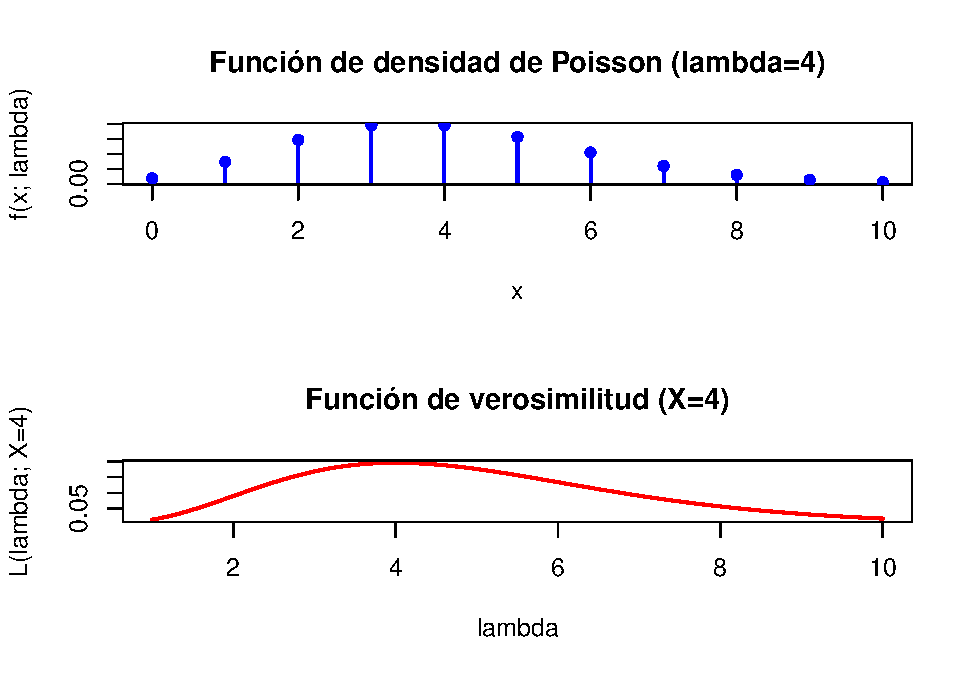
\includegraphics{EjerciciosInferenciaEstadistica_files/figure-latex/unnamed-chunk-48-1.pdf}

\begin{Shaded}
\begin{Highlighting}[]
\FunctionTok{par}\NormalTok{(opt)}
\end{Highlighting}
\end{Shaded}

\subsubsection{Explicación de los gráficos}\label{explicaciuxf3n-de-los-gruxe1ficos}

\begin{enumerate}
\def\labelenumi{\arabic{enumi}.}
\tightlist
\item
  \textbf{Función de densidad}:

  \begin{itemize}
  \tightlist
  \item
    Representa cómo varía la probabilidad de observar diferentes valores de \(x\) bajo una distribución Poisson con \(\lambda = 4\).
  \item
    Los valores de \(x\) son la variable, mientras que \(\lambda\) es constante.
  \item
    Al ser una variable discreta, la función toma valores únicamente en 0, 1, 2 etc.
  \end{itemize}
\item
  \textbf{Función de verosimilitud}:

  \begin{itemize}
  \tightlist
  \item
    Muestra cómo cambia cuan ``verosimil'' es observar el valor fijo \(X = 4\) según sean los valores de \(\lambda\).
  \item
    Aquí, \(X\) es fijo y \(\lambda\) variable.
  \item
    Es una función que toma valor para cualquier posible valor de \(\lambda\) y por tanto es continua, aunque no es una densidad.
  \end{itemize}
\end{enumerate}

\subsection{Ejercicios 6}\label{ejercicios-6}

Sean \(X_{1}, X_{2}, \ldots, X_{n}\) variables aleatorias de Bernoulli independientes tales que \(P\left(X_{i}=1\right)=p\) y \(P\left(X_{i}=\right.\) \(0)=1-p\) para cada \(i=1,2,3, \ldots\) Con la variable aleatoria \(Y\) denote el número de intentos necesario para obtener el primer éxito, es decir, el valor de \(i\) para el cual \(X_{i}=1\) ocurre primero. Entonces \(Y\) tiene una distribución geométrica con \(P(Y=y)=(1-p)^{y-1} p\), para \(y=1,2,3, \ldots\).

Encuentre el estimador del método de momentos para \(p\) basado en esta única observación de \(Y\).

\subsection{Ejercicio 7}\label{ejercicio-7-2}

Sean \(Y_{1}, Y_{2}, \ldots, Y_{n}\) variables aleatorias uniformes independientes y distribuidas idénticamente en el intervalo \((0,3 \theta)\). Deduzca el estimador del método de momentos para \(\theta\).

\subsubsection{Solución}\label{soluciuxf3n-14}

Queremos encontrar el estimador del método de momentos para el parámetro \(\theta\) basado en una muestra \(Y_1, Y_2, \ldots, Y_n\) de una distribución uniforme en el intervalo \((0, 3\theta)\).

\subsubsection{\texorpdfstring{1. Media de la distribución uniforme \((0, 3\theta)\)}{1. Media de la distribución uniforme (0, 3\textbackslash theta)}}\label{media-de-la-distribuciuxf3n-uniforme-0-3theta}

La media (es decir la esperanza matemática o momento de orden uno) de una variable aleatoria uniforme \(U(a, b)\) está dada por:

\[
\mu = \frac{a + b}{2}
\]

En este caso, los límites de la distribución son \(a = 0\) y \(b = 3\theta\), por lo que:

\[
E(Y) = \frac{0 + 3\theta}{2} = \frac{3\theta}{2}
\]

\subsubsection{2. Estimador del método de momentos}\label{estimador-del-muxe9todo-de-momentos}

El método de momentos sustituye el momento muestral correspondiente al momento poblacional en la función que relaciona el parámetro con dicho momento poblacional.

Para el primer momento, que, insistimos, es la esperanza matemática (\(E(Y^1)\) tenemos, del apartado anterior:

\[
\theta = \frac{2\cdot E(Y)}{3}
\]

Sustituyendo el primer momento poblacional, \(\mu_1= E(Y)\) por el primer momento muestral \(\hat \mu_1=\overline{Y}\), obtenemos el estimador del método de momentos:

\[
\hat{\theta} = \frac{2\overline{Y}}{3}
\]

Esto significa que para una muestra \(Y_1, Y_2, \ldots, Y_n\), podemos calcular \(\hat{\theta}\) a partir de la media muestral \(\overline{Y}\).

\subsection{Ejercicio 8}\label{ejercicio-8-2}

Sean \(Y_{1}, Y_{2}, \ldots, Y_{n}\) variables aleatorias independientes y distribuidas idénticamente de una familia de distribución de potencias con parámetros \(\alpha\) y \(\theta=3\). Entonces, si \(\alpha>0\),

\[
f(y \mid \alpha)= \begin{cases}\alpha y^{\alpha-1} / 3^{\alpha}, & 0 \leq y \leq 3 \\ 0, & \text { en cualquier otro punto.. }\end{cases}
\]

Asumiendo que hemos calculado \(E\left(Y_{1}\right)=3 \alpha /(\alpha+1)\) deduzca el estimador del método de momentos para \(\alpha\).

\subsection{Ejercicio 9}\label{ejercicio-9-1}

Suponga que \(Y_{1}, Y_{2}, \ldots, Y_{n}\) denotan una muestra aleatoria de la distribución de Poisson con media \(\lambda\).

\begin{enumerate}
\def\labelenumi{\arabic{enumi}.}
\tightlist
\item
  Encuentre el estimador máximo verosímil (EMV) \(\hat{\lambda}\) para \(\lambda\).
\item
  Encuentre el valor esperado y la varianza de \(\hat{\lambda}\).
\item
  Demuestre que el estimador del inciso a es consistente para \(\lambda\).
\item
  ¿Cuál es el EMV para \(P(Y=0)=e^{-\lambda}\) ?
\end{enumerate}

\subsubsection{Solución}\label{soluciuxf3n-15}

\paragraph{Estimador máximo verosímil (EMV)}\label{estimador-muxe1ximo-verosuxedmil-emv}

La función de verosimilitud para una muestra aleatoria de tamaño \(n\) es:

\[
L(\lambda; Y_1, \ldots, Y_n) = \prod_{i=1}^n \frac{\lambda^{Y_i} e^{-\lambda}}{Y_i!}
\]

Tomando el logaritmo de la función de verosimilitud:

\[
\ell(\lambda) = \sum_{i=1}^n \left(Y_i \ln(\lambda) - \lambda - \ln(Y_i!)\right)
\]

Derivamos con respecto a \(\lambda\) e igualamos a 0 para encontrar el EMV:

\[
\frac{\partial \ell(\lambda)}{\partial \lambda} = \sum_{i=1}^n \frac{Y_i}{\lambda} - n = 0
\]

Resolviendo para \(\lambda\), obtenemos:

\[
\hat{\lambda} = \frac{\sum_{i=1}^n Y_i}{n} = \overline{Y}
\]

Por lo tanto, el estimador máximo verosímil de \(\lambda\) es:

\[
\hat{\lambda} = \overline{Y}
\]

Estrictamente hablando, para comprobar que el valor obtenido es un máximo debemos verificar que la segunda derivada log-verosimilitud con respecto a \(\lambda\) es negativa en \(\hat{\lambda}\).

\paragraph{Segunda derivada de la log-verosimilitud}\label{segunda-derivada-de-la-log-verosimilitud}

La función log-verosimilitud es:

\[
\ell(\lambda) = \sum_{i=1}^n \left(Y_i \ln(\lambda) - \lambda - \ln(Y_i!)\right)
\]

Hemos visto que la primera derivada con respecto a \(\lambda\) es:

\[
\frac{\partial \ell(\lambda)}{\partial \lambda} = \sum_{i=1}^n \frac{Y_i}{\lambda} - n
\]

Por lo que, volviendo a derivar respecto a \(\lambda\) se obtiene:

\[
\frac{\partial^2 \ell(\lambda)}{\partial \lambda^2} = \sum_{i=1}^n \frac{-Y_i}{\lambda^2}
\]

Evaluandola en \(\hat{\lambda}\), es decir, sustituyendo \(\lambda = \hat{\lambda} = \overline{Y}\) en la segunda derivada:

\[
\frac{\partial^2 \ell(\hat{\lambda})}{\partial \lambda^2} = \sum_{i=1}^n \frac{-Y_i}{\overline{Y}^2}
\]

Dado que \(\overline{Y} = \frac{\sum_{i=1}^n Y_i}{n}\), se tiene que \(Y_i / \overline{Y}\) es positivo para todos los \(i\). Por lo tanto:

\[
\frac{\partial^2 \ell(\hat{\lambda})}{\partial \lambda^2} = \frac{-1}{\overline{Y}^2} \sum_{i=1}^n Y_i
\]

Como \(\overline{Y}\) y \(\sum_{i=1}^n Y_i\) son positivos, la segunda derivada es negativa:

\[
\frac{\partial^2 \ell(\hat{\lambda})}{\partial \lambda^2} < 0
\]

y, por lo tanto
se confirma que \(\hat{\lambda}\) es un máximo local para la función log-verosimilitud. Esto valida que el estimador encontrado es el estimador máximo verosímil (EMV).

\paragraph{\texorpdfstring{Valor esperado y varianza de \(\hat{\lambda}\)}{Valor esperado y varianza de \textbackslash hat\{\textbackslash lambda\}}}\label{valor-esperado-y-varianza-de-hatlambda}

\subparagraph{Valor esperado:}\label{valor-esperado}

Dado que \(\hat{\lambda} = \overline{Y}\) y \(\overline{Y}\) es la media muestral de variables Poisson con media \(\lambda\), tenemos:

\[
E(\hat{\lambda}) = E(\overline{Y}) = \lambda
\]

Por lo tanto, \(\hat{\lambda}\) es un estimador \textbf{insesgado} de \(\lambda\).

\subparagraph{Varianza:}\label{varianza}

La varianza de la media muestral \(\overline{Y}\) es:

\[
\text{Var}(\hat{\lambda}) = \text{Var}(\overline{Y}) = \frac{\text{Var}(Y)}{n}
\]

Dado que \(Y \sim \text{Poisson}(\lambda)\), la varianza de \(Y\) es \(\lambda\), por lo que:

\[
\text{Var}(\hat{\lambda}) = \frac{\lambda}{n}
\]

\paragraph{Consistencia del estimador}\label{consistencia-del-estimador}

Un estimador es consistente si:

\begin{enumerate}
\def\labelenumi{\arabic{enumi}.}
\tightlist
\item
  Es insesgado.
\item
  Su varianza tiende a 0 cuando \(n \to \infty\).
\end{enumerate}

De los resultados anteriores:

\begin{itemize}
\tightlist
\item
  \(E(\hat{\lambda}) = \lambda\), por lo que es insesgado.
\item
  \(\text{Var}(\hat{\lambda}) = \frac{\lambda}{n}\), que tiende a 0 cuando \(n \to \infty\).
\end{itemize}

Por lo tanto, \(\hat{\lambda}\) es un estimador \textbf{consistente} de \(\lambda\).

\paragraph{\texorpdfstring{EMV para \(P(Y = 0) = e^{-\lambda}\)}{EMV para P(Y = 0) = e\^{}\{-\textbackslash lambda\}}}\label{emv-para-py-0-e-lambda}

La probabilidad de \(Y = 0\) en una distribución Poisson es:

\[
P(Y = 0) = e^{-\lambda}
\]

El EMV de una función momótona de un parámetro es la misma función del EMV del parámetro.

Aplicando esta propiedad, que se conoce como \_invariancia funcional del EMV a la función \(h(\lambda)= P(Y = 0)= e^{-\lambda}\) se obtiene, reemplazando \(\lambda\) por su estimador EMV \(\hat{\lambda} = \overline{Y}\) el estimador ma´aximo verosimil de \(h(\lambda)\), es decir:

\[
\widehat{h(\lambda)} =
\widehat{P(Y=0)} = e^{-\hat{\lambda}} = e^{-\overline{Y}}=h(\hat\lambda)
\]

\paragraph{Resumiendo:}\label{resumiendo}

\begin{enumerate}
\def\labelenumi{\arabic{enumi}.}
\tightlist
\item
  El estimador máximo verosímil de \(\lambda\) es \(\hat{\lambda} = \overline{Y}\).
\item
  El valor esperado de \(\hat{\lambda}\) es \(E(\hat{\lambda}) = \lambda\), y su varianza es \(\text{Var}(\hat{\lambda}) = \frac{\lambda}{n}\).
\item
  \(\hat{\lambda}\) es un estimador consistente para \(\lambda\).
\item
  El EMV de \(P(Y = 0)\) es \(\widehat{P(Y = 0)} = e^{-\overline{Y}}\).
\end{enumerate}

\subsection{Ejercicio 10}\label{ejercicio-10-1}

Suponga que \(Y_{1}, Y_{2}, \ldots, Y_{n}\) denotan una muestra aleatoria de una población distribuida exponencialmente con media \(\theta\). Encuentre el MLE de la varianza poblacional \(\theta^{2}\).

\section{Intervalos de confianza}\label{intervalos-de-confianza}

\subsection{PROBLEMA 1}\label{problema-1-1}

La distribución del número de huevos puestos por una determinada especie de gallina durante su período de reproducción tiene una media de 35 huevos con una desviación estándar de 18.2. Supongamos que un grupo de investigadores recoge una muestra aleatoria de 45 gallinas de esta especie, cuenta el número de huevos establecidos durante el período de reproducción y registra la media de la muestra. Repiten estas muestras 1.000 veces, y construyen una distribución de las medias de la muestra.

\begin{enumerate}
\def\labelenumi{\alph{enumi})}
\tightlist
\item
  ¿Cómo se llama esta distribución?\\
\item
  ¿Esperaríamos que la forma de esta distribución fuera simétrica, sesgada o no sesgada? Razona la respuesta.\\
\item
  Calcula la variabilidad de esta distribución y di cómo se llama el parámetro que la mide.\\
\item
  Supongamos que el presupuesto de los investigadores se reduce y solo pueden recoger muestras aleatorias de 10 gallinas. Se registra la media de las muestras del número de huevos y se repite 1.000 veces, construyendo una nueva distribución de las medias de la muestra. ¿Cómo será la variabilidad de esta nueva distribución comparada con la variabilidad de la distribución original?
\end{enumerate}

\subsection{PROBLEMA 2}\label{problema-2-1}

Un administrador de hospital con la esperanza de mejorar los tiempos de espera decide estimar el tiempo de espera medio de la sala de urgencias (ER) de su hospital. Recopila una muestra aleatoria simple de 64 pacientes y determina el tiempo (en minutos) entre cuando ingresaron al ER hasta que fueron visitados por un médico. Un intervalo de confianza del 95\% basado en esta muestra es (128 minutos, 147 minutos), basado en una distribución normal para la media. Determina y razona si las siguientes afirmaciones son verdaderas o falsas.

\begin{enumerate}
\def\labelenumi{\alph{enumi})}
\tightlist
\item
  Este intervalo de confianza no es válido, ya que no sabemos si la distribución en la población de los tiempos de espera de ER es normal.\\
\item
  Tenemos una confianza del 95\% de que el tiempo de espera medio de estos 64 pacientes en una sala de emergencias está entre 128 y 147 minutos.\\
\item
  Tenemos una confianza del 95\% de que el tiempo de espera medio de todos los pacientes en la sala de emergencias de este hospital está entre 128 y 147 minutos.\\
\item
  El 95\% de las muestras aleatorias tienen una media muestral entre 128 y 147 minutos.\\
\item
  Un intervalo de confianza del 99\% sería más estrecho que el intervalo de confianza del 95\%, ya que debemos estar más seguros de nuestra estimación.\\
\item
  El margen de error es de 9,5 y la media de la muestra es de 137,5.\\
\item
  Para reducir el margen de error de un intervalo de confianza del 95\% a la mitad de lo que es ahora, tendremos que duplicar el tamaño de la muestra.
\end{enumerate}

\subsubsection{SOLUCIÓN}\label{soluciuxf3n-16}

Aquí tienes la traducción de las respuestas al castellano:

\begin{enumerate}
\def\labelenumi{\alph{enumi})}
\item
  Falso. El tamaño muestral permite aceptar la normalidad por el TLC.
\item
  Falso. La inferencia se realiza sobre el parámetro poblacional, no sobre el parámetro muestral, que siempre estará dentro del intervalo.
\item
  Cierto.
\item
  Falso. No hacemos inferencia sobre las muestras.
\item
  Falso. Sería más amplio.
\item
  Cierto. La media es el punto medio del intervalo.
\item
  Falso. Deberíamos cuadruplicar el tamaño de la muestra.
\end{enumerate}

\subsection{PROBLEMA 3}\label{problema-3-1}

Las autoridades sanitarias fijan la cantidad de 14 UFP/100ml (UFP=unidades formadoras de placas) como la concentración máxima de un determinado virus entérico en aguas residuales de cualquier punto del estado. Se realiza un control en aguas depuradas de 10 granjas que generan purines. La concentración del virus entérico corresponde a un número muy grande, de forma que podemos asumir que sigue una distribución Normal. Por otro lado, las granjas están suficientemente alejadas como para asumir que los resultados individuales son mutuamente independientes.

Los valores obtenidos han sido:

\begin{longtable}[]{@{}lllllllll@{}}
\toprule\noalign{}
14.3 & 15.3 & 13.8 & 15.4 & 15.5 & 14.6 & 13.9 & 15 & 14 \\
\midrule\noalign{}
\endhead
\bottomrule\noalign{}
\endlastfoot
\end{longtable}

\begin{enumerate}
\def\labelenumi{\arabic{enumi}.}
\tightlist
\item
  Calcula el intervalo de confianza al 95\% de la concentración media del virus en las aguas que vierten las granjas.\\
\item
  Interpreta el resultado en función del valor fijado por la administración.
\end{enumerate}

\subsubsection{SOLUCIÓN}\label{soluciuxf3n-17}

\paragraph{Cálculo del intervalo de confianza al 95\% para la concentración media del virus}\label{cuxe1lculo-del-intervalo-de-confianza-al-95-para-la-concentraciuxf3n-media-del-virus}

El intervalo de confianza (IC) para la media de una población normal con varianza desconocida se calcula como:

\[ \bar{x} \pm t_{n-1, 1-\alpha/2} \cdot \frac{s}{\sqrt{n}} \]

Donde:
- \(\bar{x}\) es la media muestral.
- \(t_{n-1, 1-\alpha/2}\) es el valor crítico de la distribución \(t\) de Student con \(n-1\) grados de libertad y nivel de confianza \(1-\alpha\).
- \(s\) es la desviación estándar muestral.
- \(n\) es el tamaño de la muestra.

Los datos proporcionados son:

\[ \text{concentración} = \{14.3, 15.3, 13.8, 15.4, 15.5, 14.6, 13.9, 15.0, 14.6, 13.8\} \]

El tamaño muestral es \(n=10\). Calculamos la media (\(\bar{x}\)) y la desviación estándar (\(s\)) con R y usamos la función \texttt{t.test} para obtener el intervalo de confianza.

\begin{Shaded}
\begin{Highlighting}[]
\CommentTok{\# Datos}
\NormalTok{conc\_virus }\OtherTok{\textless{}{-}} \FunctionTok{c}\NormalTok{(}\FloatTok{14.3}\NormalTok{, }\FloatTok{15.3}\NormalTok{, }\FloatTok{13.8}\NormalTok{, }\FloatTok{15.4}\NormalTok{, }\FloatTok{15.5}\NormalTok{, }\FloatTok{14.6}\NormalTok{, }\FloatTok{13.9}\NormalTok{, }\FloatTok{15.0}\NormalTok{, }\FloatTok{14.6}\NormalTok{, }\FloatTok{13.8}\NormalTok{)}

\CommentTok{\# Intervalo de confianza al 95\%}
\NormalTok{res }\OtherTok{\textless{}{-}} \FunctionTok{t.test}\NormalTok{(conc\_virus)}
\NormalTok{res}\SpecialCharTok{$}\NormalTok{conf.int}
\end{Highlighting}
\end{Shaded}

\begin{verbatim}
## [1] 14.14573 15.09427
## attr(,"conf.level")
## [1] 0.95
\end{verbatim}

Resultados obtenidos:
- Límite inferior del IC: 14.1457
- Límite superior del IC: 15.0943

Por lo tanto, el intervalo de confianza al 95\% es:

\[ (14.146, 15.094) \]

\begin{center}\rule{0.5\linewidth}{0.5pt}\end{center}

\paragraph{Interpretación del resultado}\label{interpretaciuxf3n-del-resultado-3}

El valor fijado por la administración como límite máximo aceptable para la concentración de virus es 14 UFP/100ml. Observamos que \textbf{todo el intervalo de confianza calculado está por encima de este valor (14.146, 15.094)}. Esto implica que:

\begin{itemize}
\tightlist
\item
  Es razonable concluir que la media poblacional de la concentración del virus está por encima de 14 UFP/100ml.
\item
  Solo el 5\% de los intervalos que construimos a partir de muestras no contiene la verdadera media poblacional, y el intervalo que hemos construido no incluye el valor fijado por la administración.
\end{itemize}

\textbf{Conclusión}: Existe evidencia estadística para sugerir, con una alta confianza, que las granjas exceden, en promedio, el límite permitido por las autoridades sanitarias.

\subsection{PROBLEMA 4}\label{problema-4-1}

En un estudio sobre los efectos fisiológicos del alcohol se midió el tiempo que se tarda en reaccionar a un estímulo en un conjunto de seis individuos antes y después de consumir una fuerte dosis de alcohol. El tiempo de latencia medido en milisegundos fue el siguiente:

\begin{longtable}[]{@{}lrrrrrr@{}}
\toprule\noalign{}
Individuo & 1 & 2 & 3 & 4 & 5 & 6 \\
\midrule\noalign{}
\endhead
\bottomrule\noalign{}
\endlastfoot
Antes & 3.85 & 3.81 & 3.60 & 3.68 & 3.78 & 3.83 \\
Después & 3.82 & 3.95 & 3.80 & 3.87 & 3.88 & 3.94 \\
\end{longtable}

\begin{enumerate}
\def\labelenumi{\alph{enumi})}
\item
  Calcula un intervalo de confianza del 95\% para la diferencia de medias: \emph{Después - Antes}.\\
  ¿Podríamos afirmar que la media después es superior a la media antes?
\item
  ¿Cómo cambiará el intervalo si reducimos el nivel de confianza al 90\%?\\
  ¿Será más amplio? ¿Será más estrecho? ¿O no cambiará?
\end{enumerate}

\subsubsection{SOLUCIÓN}\label{soluciuxf3n-18}

\paragraph{\texorpdfstring{Cálculo del intervalo de confianza al 95\% para la diferencia de medias: \emph{Después - Antes}}{Cálculo del intervalo de confianza al 95\% para la diferencia de medias: Después - Antes}}\label{cuxe1lculo-del-intervalo-de-confianza-al-95-para-la-diferencia-de-medias-despuuxe9s---antes}

Estamos trabajando con datos apareados, ya que se trata de mediciones realizadas en los mismos individuos antes y después de consumir alcohol. Por lo tanto, calculamos las diferencias entre los valores \emph{Después - Antes} para cada individuo, y procedemos como si fuera un problema de una sola muestra con las diferencias.

El intervalo de confianza para la media de las diferencias se calcula como:

\[ \bar{d} \pm t_{n-1, 1-\alpha/2} \cdot \frac{s_d}{\sqrt{n}} \]

Donde:
- \(\bar{d}\) es la media de las diferencias.
- \(t_{n-1, 1-\alpha/2}\) es el valor crítico de la distribución \(t\) de Student con \(n-1\) grados de libertad y nivel de confianza \(1-\alpha\).
- \(s_d\) es la desviación estándar de las diferencias.
- \(n\) es el número de pares.

Los datos son:
- Antes: \([3.85, 3.81, 3.60, 3.68, 3.78, 3.83]\)
- Después: \([3.82, 3.95, 3.80, 3.87, 3.88, 3.94]\)

Calculemos el intervalo de confianza al 95\% con R.

\begin{Shaded}
\begin{Highlighting}[]
\CommentTok{\# Datos}
\NormalTok{antes }\OtherTok{\textless{}{-}} \FunctionTok{c}\NormalTok{(}\FloatTok{3.85}\NormalTok{, }\FloatTok{3.81}\NormalTok{, }\FloatTok{3.60}\NormalTok{, }\FloatTok{3.68}\NormalTok{, }\FloatTok{3.78}\NormalTok{, }\FloatTok{3.83}\NormalTok{)}
\NormalTok{despues }\OtherTok{\textless{}{-}} \FunctionTok{c}\NormalTok{(}\FloatTok{3.82}\NormalTok{, }\FloatTok{3.95}\NormalTok{, }\FloatTok{3.80}\NormalTok{, }\FloatTok{3.87}\NormalTok{, }\FloatTok{3.88}\NormalTok{, }\FloatTok{3.94}\NormalTok{)}

\CommentTok{\# Intervalo de confianza al 95\% para las diferencias pareadas}
\NormalTok{res\_95 }\OtherTok{\textless{}{-}} \FunctionTok{t.test}\NormalTok{(despues, antes, }\AttributeTok{paired =} \ConstantTok{TRUE}\NormalTok{)}
\NormalTok{res\_95}\SpecialCharTok{$}\NormalTok{conf.int}
\end{Highlighting}
\end{Shaded}

\begin{verbatim}
## [1] 0.03092935 0.20573732
## attr(,"conf.level")
## [1] 0.95
\end{verbatim}

Resultados:
- Límite inferior del IC: 0.03093
- Límite superior del IC: 0.20574

El intervalo de confianza al 95\% para la diferencia de medias es:

\[ (0.031, 0.206) \]

\textbf{Interpretación}: Como todo el intervalo está en la parte positiva de la recta real, podemos afirmar con un 95\% de confianza que la media después de consumir alcohol es superior a la media antes de consumir alcohol.

\paragraph{Cambio del intervalo al reducir el nivel de confianza al 90\%}\label{cambio-del-intervalo-al-reducir-el-nivel-de-confianza-al-90}

Al reducir el nivel de confianza al 90\%, el valor crítico \(t_{n-1, 1-\alpha/2}\) disminuye, lo que hace que el intervalo de confianza sea más estrecho. Calculemos el nuevo intervalo con R.

\begin{Shaded}
\begin{Highlighting}[]
\CommentTok{\# Intervalo de confianza al 90\% para las diferencias pareadas}
\NormalTok{res\_90 }\OtherTok{\textless{}{-}} \FunctionTok{t.test}\NormalTok{(despues, antes, }\AttributeTok{paired =} \ConstantTok{TRUE}\NormalTok{, }\AttributeTok{conf.level =} \FloatTok{0.9}\NormalTok{)}
\NormalTok{res\_90}\SpecialCharTok{$}\NormalTok{conf.int}
\end{Highlighting}
\end{Shaded}

\begin{verbatim}
## [1] 0.0498184 0.1868483
## attr(,"conf.level")
## [1] 0.9
\end{verbatim}

Resultados:
- Límite inferior del IC: 0.04982
- Límite superior del IC: 0.18685

El intervalo de confianza al 90\% es:

\[ (0.050, 0.187) \]

\textbf{Conclusión}: Como esperábamos, el intervalo al 90\% es más estrecho que el intervalo al 95\%. Esto ocurre porque reducimos el nivel de confianza, lo que implica un menor margen de error.

\subsection{PROBLEMA 5}\label{problema-5-1}

El estudio sanguíneo de un individuo presenta 125 neutrófilos de un recuento total de 200 glóbulos blancos. Se pide:

\begin{enumerate}
\def\labelenumi{\arabic{enumi}.}
\tightlist
\item
  Encuentra una estimación puntual para la proporción de neutrófilos.\\
\item
  Encuentra un intervalo de confianza al 90\% para la anterior proporción.\\
\item
  En un individuo sano, el porcentaje de neutrófilos se encuentra entre el 60\% y el 70\% del total de glóbulos blancos. Según el intervalo del apartado anterior, ¿hay alguna evidencia de desequilibrio de neutrófilos en la muestra de sangre analizada?
\end{enumerate}

\subsubsection{SOLUCIÓN}\label{soluciuxf3n-19}

\paragraph{Estimación puntual para la proporción de neutrófilos}\label{estimaciuxf3n-puntual-para-la-proporciuxf3n-de-neutruxf3filos}

El estimador (por momentos y por máxima verosimilitud) de la proporción poblacional es la frecuencia relativa (\(\hat{p}\)) que se calcula como:

\[ \hat{p} = \frac{x}{n} \]

Donde:
- \(x = 125\) es el número de neutrófilos.
- \(n = 200\) es el total de glóbulos blancos.

Calculamos \(\hat{p}\):

\begin{Shaded}
\begin{Highlighting}[]
\CommentTok{\# Datos}
\NormalTok{x }\OtherTok{\textless{}{-}} \DecValTok{125}
\NormalTok{n }\OtherTok{\textless{}{-}} \DecValTok{200}

\CommentTok{\# Proporción muestral}
\NormalTok{p\_hat }\OtherTok{\textless{}{-}}\NormalTok{ x }\SpecialCharTok{/}\NormalTok{ n}
\NormalTok{p\_hat}
\end{Highlighting}
\end{Shaded}

\begin{verbatim}
## [1] 0.625
\end{verbatim}

Resultado:
\[ \hat{p} = 0.625 \]

La estimación puntual para la proporción de neutrófilos es \textbf{0.625} o \textbf{62.5\%}.

\paragraph{Intervalo de confianza al 90\% para la proporción}\label{intervalo-de-confianza-al-90-para-la-proporciuxf3n}

El intervalo de confianza asintótico para una proporción se calcula como:

\[ \hat{p} \pm z_{1-\alpha/2} \cdot \sqrt{\frac{\hat{p}(1-\hat{p})}{n}} \]

Donde:

\begin{itemize}
\tightlist
\item
  \(z_{1-\alpha/2}\) es el valor crítico de la distribución normal estándar para un nivel de confianza del 90\%.
\item
  \(\hat{p}\) es la proporción muestral.
\item
  \(n\) es el tamaño de la muestra.
\end{itemize}

Usamos R para calcular este intervalo:

\begin{Shaded}
\begin{Highlighting}[]
\CommentTok{\# Nivel de confianza}
\NormalTok{alpha }\OtherTok{\textless{}{-}} \FloatTok{0.1}
\NormalTok{z }\OtherTok{\textless{}{-}} \FunctionTok{qnorm}\NormalTok{(}\DecValTok{1} \SpecialCharTok{{-}}\NormalTok{ alpha }\SpecialCharTok{/} \DecValTok{2}\NormalTok{)}

\CommentTok{\# Error estándar}
\NormalTok{se }\OtherTok{\textless{}{-}} \FunctionTok{sqrt}\NormalTok{(p\_hat }\SpecialCharTok{*}\NormalTok{ (}\DecValTok{1} \SpecialCharTok{{-}}\NormalTok{ p\_hat) }\SpecialCharTok{/}\NormalTok{ n)}

\CommentTok{\# Intervalo de confianza}
\NormalTok{lower }\OtherTok{\textless{}{-}}\NormalTok{ p\_hat }\SpecialCharTok{{-}}\NormalTok{ z }\SpecialCharTok{*}\NormalTok{ se}
\NormalTok{upper }\OtherTok{\textless{}{-}}\NormalTok{ p\_hat }\SpecialCharTok{+}\NormalTok{ z }\SpecialCharTok{*}\NormalTok{ se}
\FunctionTok{c}\NormalTok{(lower, upper)}
\end{Highlighting}
\end{Shaded}

\begin{verbatim}
## [1] 0.5686923 0.6813077
\end{verbatim}

Resultado:
- Límite inferior: \textbf{0.569}
- Límite superior: \textbf{0.681}

El intervalo de confianza al 90\% para la proporción de neutrófilos es:

\[ (0.569, 0.681) \]

\paragraph{Evidencia de desequilibrio de neutrófilos}\label{evidencia-de-desequilibrio-de-neutruxf3filos}

Un individuo sano tiene una proporción de neutrófilos entre 60\% y 70\% (\(0.6 \leq p \leq 0.7\)). Observamos que:

\begin{itemize}
\item
  El intervalo de confianza calculado es \((0.569, 0.681)\).
\item
  Dado que hay una considerable superposición entre ambos intervalos no podemos concluir que haya evidencia de desequilibrio de neutrófilos.
\end{itemize}

\subsection{PROBLEMA 6}\label{problema-6}

Un proceso químico se lleva a cabo usando un catalizador del que se quiere estimar el rendimiento medio. Una muestra piloto de tamaño 8 estima la desviación típica con un valor de 2.

Decide el tamaño de muestra necesario para obtener intervalos de confianza para la media con un 90\% y un 95\% de confianza de anchura igual a 3 (precisión 1.5), suponiendo que dicha variable sigue un modelo normal.

\subsubsection{SOLUCIÓN}\label{soluciuxf3n-20}

Queremos determinar el tamaño de muestra necesario para obtener intervalos de confianza para la media con anchura igual a 3 (precisión de 1.5), considerando niveles de confianza del 90\% y 95\%. Se sabe que la desviación estándar estimada del proceso químico es \(\sigma = 2\) y que la variable sigue una distribución normal.

Dado que la desviación estándar es estimada, nos basaremos en la distribución \(t\) de Student en lugar de la normal estándar.

La amplitud del intervalo de confianza para la media basado en la distribución \(t\) se calcula como:

\[ \text{Amplitud} = 2 \cdot t_{n-1, 1-\alpha/2} \cdot \frac{\sigma}{\sqrt{n}} \]

Resolviendo para \(n\), a partir de la precisión, es decir la mitad de la amplitud se tiene:

\[ n = \left( \frac{t_{n-1, 1-\alpha/2} \cdot \sigma}{\text{Precisión}} \right)^2 \]

Donde:
- \(\text{Precisión} = \frac{\text{Anchura}}{2} = 1.5\).
- \(t_{n-1, 1-\alpha/2}\) es el valor crítico de la distribución \(t\) con \(n-1\) grados de libertad y nivel de confianza \(1-\alpha\).
- \(\sigma = 2\) es la desviación estándar estimada.

Como \(t_{n-1, 1-\alpha/2}\) depende de \(n\), este cálculo requiere iteración.

Realizaremos manualmente la iteración aunque también es posible usar algun paquete como \texttt{DescTools} para confirmar los resultados.

\paragraph{Cálculo manual con iteración}\label{cuxe1lculo-manual-con-iteraciuxf3n}

Dado que para un valor fijo de \(\alpha\) el valor de \(t\) depende de \(n\) podemos iterar para calcular \(n\), ajustando el valor de \(t_{n-1, 1-\alpha/2}\) en cada paso según el tamaño de muestra estimado.

Podemos empezar con un valor bien bajo de \(n\) y, a partir de éste ir aumentando el tamaño.

\begin{Shaded}
\begin{Highlighting}[]
\NormalTok{s }\OtherTok{\textless{}{-}} \DecValTok{2}          \CommentTok{\# Desviación estándar}
\NormalTok{precision }\OtherTok{\textless{}{-}} \FloatTok{1.5}  \CommentTok{\# Precisión deseada}

\NormalTok{find\_n }\OtherTok{\textless{}{-}} \ControlFlowTok{function}\NormalTok{(conf\_level) \{}
\NormalTok{  n }\OtherTok{\textless{}{-}} \DecValTok{4}  \CommentTok{\# Tamaño inicial}
  \ControlFlowTok{repeat}\NormalTok{ \{}
\NormalTok{    t\_value }\OtherTok{\textless{}{-}} \FunctionTok{qt}\NormalTok{(}\DecValTok{1} \SpecialCharTok{{-}}\NormalTok{ (}\DecValTok{1} \SpecialCharTok{{-}}\NormalTok{ conf\_level) }\SpecialCharTok{/} \DecValTok{2}\NormalTok{, }\AttributeTok{df =}\NormalTok{ n }\SpecialCharTok{{-}} \DecValTok{1}\NormalTok{)}
\NormalTok{    n\_new }\OtherTok{\textless{}{-}} \FunctionTok{ceiling}\NormalTok{((t\_value }\SpecialCharTok{*}\NormalTok{ s }\SpecialCharTok{/}\NormalTok{ precision)}\SpecialCharTok{\^{}}\DecValTok{2}\NormalTok{)}
    \ControlFlowTok{if}\NormalTok{ (n\_new }\SpecialCharTok{==}\NormalTok{ n) }\ControlFlowTok{break}
\NormalTok{    n }\OtherTok{\textless{}{-}}\NormalTok{ n\_new}
\NormalTok{  \}}
  \FunctionTok{return}\NormalTok{(n)}
\NormalTok{\}}

\CommentTok{\# Tamaños de muestra para 90\% y 95\%}
\NormalTok{n\_90\_iter }\OtherTok{\textless{}{-}} \FunctionTok{find\_n}\NormalTok{(}\FloatTok{0.90}\NormalTok{)}
\NormalTok{n\_95\_iter }\OtherTok{\textless{}{-}} \FunctionTok{find\_n}\NormalTok{(}\FloatTok{0.95}\NormalTok{)}
\FunctionTok{c}\NormalTok{(n\_90\_iter, n\_95\_iter)}
\end{Highlighting}
\end{Shaded}

\begin{verbatim}
## [1]  7 10
\end{verbatim}

Resultados del cálculo iterativo:
1. Para un nivel de confianza del \textbf{90\%}, \(n =\) 7.
2. Para un nivel de confianza del \textbf{95\%}, \(n =\) 10.

Al aumentar el nivel de confianza del 90\% al 95\%, el tamaño de muestra necesario aumenta debido al incremento del valor crítico \(t\), lo que refleja una mayor necesidad de datos para reducir la incertidumbre del intervalo.

\subsection{PROBLEMA 7}\label{problema-7}

En un estudio sobre las alteraciones hormonales que se presentan durante la práctica deportiva se ha medido el aumento de cortisol al realizar una prueba específica de resistencia de 30 minutos. El trabajo se ha realizado con voluntarios de edad y peso similares, pero diferenciados según sus hábitos, separando en dos grupos a los participantes: sedentarios y practicantes habituales de algún deporte. Se supone que la variable medida sigue el modelo normal con varianza común. Se han medido 8 personas de cada grupo.

Se han publicado los siguientes intervalos de confianza (con nivel de confianza del 90\%):

\begin{itemize}
\tightlist
\item
  Sedentarios: \((2.85,4.40)\)\\
\item
  Practicantes de deporte: \((3.52,5.23)\)
\end{itemize}

\begin{enumerate}
\def\labelenumi{\alph{enumi})}
\tightlist
\item
  Calcula las medias muestrales de cada grupo.\\
\item
  Si la concentración está expresada en \(\mu \mu \mathrm{g} / \mathrm{dl}\) (microgramos por decilitro) y suponemos que se prefiere finalmente presentar los resultados en \(\mathrm{ng} / \mathrm{ml}\) (nanogramos por mililitro), ¿cómo quedarían afectados los intervalos de confianza iniciales?
\end{enumerate}

\subsection{PROBLEMA 8}\label{problema-8}

Se reporta el siguiente listado del análisis del nivel de colesterol en una muestra de 30 individuos obesos. Desafortunadamente, algunas partes del listado se han vuelto ilegibles y su valor se ha sustituido por 9999.

\begin{Shaded}
\begin{Highlighting}[]
\NormalTok{One Sample t}\SpecialCharTok{{-}}\NormalTok{test}
\NormalTok{data}\SpecialCharTok{:}\NormalTok{ x}
\NormalTok{t }\SpecialCharTok{$}\ErrorTok{=}\FloatTok{301.49}\SpecialCharTok{$}\NormalTok{, df }\SpecialCharTok{$}\ErrorTok{=}\DecValTok{9999}\NormalTok{, \textbackslash{}mathrm\{p\}}\SpecialCharTok{${-}}\NormalTok{value }\SpecialCharTok{$}\ErrorTok{\textless{}}\FloatTok{2.2}\NormalTok{ \textbackslash{}mathrm\{e\}}\SpecialCharTok{{-}}\DecValTok{16}\SpecialCharTok{$}
\NormalTok{alternative hypothesis}\SpecialCharTok{:}\NormalTok{ true mean is not equal to }\DecValTok{0}
\DecValTok{95}\NormalTok{ percent confidence interval}\SpecialCharTok{:}
\FloatTok{246.8329999}\NormalTok{ .}\DecValTok{000}
\NormalTok{sample estimates}\SpecialCharTok{:}
\NormalTok{mean of x}
\FloatTok{248.5179}
\end{Highlighting}
\end{Shaded}

Reconstruye los valores incorrectos del listado.

\end{document}
